 \documentclass[11pt,a4paper,twoside]{tesis}
% SI NO PENSAS IMPRIMIRLO EN FORMATO LIBRO PODES USAR
%\documentclass[11pt,a4paper]{tesis}

\usepackage{graphicx}
\usepackage[utf8]{inputenc}
\usepackage[spanish]{babel}
\usepackage[left=3cm,right=3cm,bottom=3.5cm,top=3.5cm]{geometry}
\usepackage[square,sort,comma,numbers]{natbib}
\usepackage{hyperref}
\usepackage{booktabs}
\usepackage{multirow}
\usepackage{amsmath}
\usepackage{tabularx}
\usepackage{todonotes}

\setlength{\marginparwidth}{2cm}

\bibliographystyle{plainnat}

\begin{document}

%%%% CARATULA

\def\autor{Juan Manuel Pérez}
\def\tituloTesis{Técnicas y recursos para la detección automática de lenguaje discriminatorio en redes sociales}
\def\runtitulo{Técnicas y recursos para la detección automática de lenguaje discriminatorio en redes sociales}
\def\runtitle{Techniques and resources for the automatic detection of hate speech in social networks}
\def\director{Franco Luque}
\def\codirector{Agustín Gravano}
\def\lugar{Buenos Aires, 2021}
\newcommand{\HRule}{\rule{\linewidth}{0.2mm}}
%
\thispagestyle{empty}

\begin{center}\leavevmode

    \vspace{-2cm}

    \begin{tabular}{l}
        
\includegraphics[width=2.6cm]{img/logofcen.png}
    \end{tabular}


    {\large \sc Universidad de Buenos Aires

    Facultad de Ciencias Exactas y Naturales

    Departamento de Computaci\'on}

    \vspace{6.0cm}

    %\vspace{3.0cm}
    %{
    %\Large \color{red}
    %\begin{tabular}{|p{2cm}cp{2cm}|}
    %\hline
    %& Pre-Final Version: \today &\\
    %\hline
    %\end{tabular}
    %}
    %\vspace{2.5cm}

    \begin{huge}
        \textbf{\tituloTesis}
    \end{huge}

    \vspace{2cm}

    {\large Tesis presentada para el título de Doctor de la Universidad de Buenos Aires en
        el área de Ciencias de la Computaci\'on}

    \vspace{2cm}

    {\Large \autor}

\end{center}

\vfill

{\large

    \begin{tabular}{l l}
        \vspace{.3cm} Director:              & Dr. Franco Luque                    \\
        \vspace{.3cm} Director Asistente:    & Dr. Agustín Gravano                 \\
        \vspace{.3cm} Consejero de Estudios: & Dr. Diego Fernández Slezak          \\
        Lugar de Trabajo:                    & Departamento de Computación         \\
                                             & Facultad de Cs. Exactas y Naturales \\
        \vspace{1cm}                         & Universidad de Buenos Aires         \\
        Buenos Aires, 2022                   &                                     \\
    \end{tabular}

    \vspace{.2cm}



    \vspace{.2cm}


}

\newpage\thispagestyle{empty}


%%%% ABSTRACTS, AGRADECIMIENTOS Y DEDICATORIA
\frontmatter
\pagestyle{empty}
%\begin{center}
%\large \bf \runtitulo
%\end{center}
%\vspace{1cm}
\chapter*{\runtitulo}

{

    \setstretch{1.5}

\noindent El discurso discriminatorio (también conocido como discurso de odio) puede describirse como aquel discurso en clave de intenso aborrecimiento, denigración y enemistad que ataca a un individuo o un grupo de individuos por poseer –o aparentar poseer– cierta característica protegida por tratados internacionales como el sexo, el género, la etnia, etc. En los últimos años, este tipo de discurso ha tomado gran relevancia en redes sociales y otros medios virtuales debido a su intensidad y a su relación con actos violentos contra miembros de estos grupos. A raíz de esto, estados y organizaciones supranacionales como la Unión Europea han sancionado legislación que insta a las empresas de redes sociales a moderar y eliminar contenido discriminatorio, con particular foco en aquel que insta a la violencia física.

Debido a la enorme cantidad de contenido generado por usuarios en las redes sociales, es necesario contar con cierta automatización en esta tarea, bien para su análisis o para su moderación. Desde la óptica del procesamiento de lenguaje natural, la detección de discriminación puede entenderse como un problema de clasificación de texto: dado un texto generado por un usuario, predecir si es o no contenido discriminatorio. Así mismo, puede ser de interés predecir otras características: por ejemplo, si el texto contiene un llamado a la acción violenta, si está dirigido contra un individuo o un grupo, o el tipo de característica ofendida, entre otras.

Una de las limitaciones de los enfoques actuales para la detección del lenguaje discriminatorio es la falta de contexto en el mensaje. La mayoría de los estudios y recursos están hechos sobre datos fuera de contexto; es decir, mensajes aislados sin ningún tipo de contexto conversacional o del tema del cual se habla. Esto restringe la información disponible –tanto para un humano como para un sistema– para poder discernir si un texto social es discriminatorio. Otra información usualmente faltante es la característica atacada: es común que los datasets estén anotados de manera poco granular, no brindando información acerca de si la agresión es por motivos de sexo, género, clase social, etc. Por último, una limitación puntual del español es la poca disponibilidad de recursos para esta tarea.

En esta tesis pretendemos abordar algunas de las limitaciones marcadas. Por un lado, analizamos el impacto de agregar contexto a la detección de lenguaje discriminatorio en redes sociales. Para ello, construimos un conjunt de datos de tweets en base a las respuestas de los usuarios a los posteos de medios periodísticos en Twitter. Esto nos permite obtener dos tipos de contextos: uno “conversacional” al tener una respuesta a un tweet anterior, y otro más extenso al obtener el texto de la noticia en cuestión. El corpus fue recolectado sobre noticias relacionadas a la pandemia de COVID-19, en idioma español mayormente en su variedad dialectal rioplatense y anotado por hablantes nativos de ese dialecto con un nuevo modelo de etiquetado, que es granular respecto de las características ofendidas.

Sobre los comentarios de este dataset realizamos experimentos de detección de discurso de odio planteando dos tareas: detección binaria del lenguaje discriminatorio, donde sólo predecimos una etiqueta binaria indicando presencia de lenguaje discriminatorio; y detección granular, donde predecimos las características ofendidas. Usando técnicas del estado del arte, obtuvimos mejoras significativas en ambas tareas al agregar contexto como entrada de cada instancia, tanto en su forma corta (sólo el titular/tweet de la noticia) como en su forma larga (titular y cuerpo de la noticia). Así mismo, observamos que un clasificador entrenado para la tarea granular mejora levemente su performance al ser evaluado para la tarea binaria, obviando los posibles errores de motivos discriminatorios. Combinando la adición de contexto y granularidad, un clasificador para la detección de lenguaje discriminatorio obtiene mejoras considerables sobre un BERT en español que sólo consume el texto del comentario.

Considerando la detección de discurso de odio dentro del área más abarcativa de clasificación de documentos en dominios sociales, analizamos también algunos aspectos generales de tareas relacionadas como el análisis de sentimiento y la detección de emociones, entre otras. En particular, analizamos el desempeño de varias técnicas modernas de representación al ser entrenadas en dominios sociales. Comúnmente, los modelos de representación son entrenados a partir de textos de dominios formales, como pueden ser Wikipedia u otras fuentes similares. En esta tesis observamos que –desde los word embeddings hasta los modelos pre-entrenados basados en transformers– las representaciones generadas son robustas y mejoran la performance en un conjunto de tareas de clasificación en textos sociales. Sobre los modelos pre-entrenados, estudiamos el impacto de entrenarlos desde cero en textos sociales o efectuar una adaptación a este dominio.

Todos los estudios y recursos presentados en esta tesis fueron realizados en el idioma español. Como un objetivo secundario, pretendemos contribuir a mitigar la enorme asimetría de recursos existente en el área del procesamiento del lenguaje natural.


}


\bigskip

\noindent\textbf{Palabras claves:} Hate Speech, Natural Language Processing, Abusive Language Detection, Domain Adaptation, Social NLP.

\cleardoublepage
%\begin{center}
%\large \bf \runtitle
%\end{center}
%\vspace{1cm}
\chapter*{\runtitle}

\noindent
Hate speech can be described as speech containing intense hatred, denigration, and enmity that attacks an individual or a group of individuals because of possessing –or pretending to possess– any characteristic protected by international treaties such as gender, ethnicity, religion, language, among others. In recent years, this type of discourse has gained great relevance in social networks and other virtual media due to its intensity and its relationship with violent acts against members of these groups. As a result, states and supranational organizations –such as the European Union– have enacted legislation that urges social media companies to moderate and remove discriminatory content, with particular focus on that which promotes physical violence.

Due to the enormous amount of user-generated content on social media, it is necessary to have some degree of automation in this task, either for analysis or for moderation. From a natural language processing (NLP) perspective, hate speech detection can be understood as a text classification problem: given a text generated by a user, predict whether it is discriminatory content. Likewise, it may be of interest to predict other features: for example, if the text contains a call to violent action; if it is directed against an individual or a group; or the offended characteristic, among others.

One of the limitations of current approaches to hate speech detection is the lack of context. Most studies and resources are performed on data without context; that is, isolated messages without any type of conversational context or the topic being discussed. This restricts the information available –both for a human and for an automated system– to discern if a social text is hateful or not. Other information usually lacking is the offended characteristic: datasets are usually annotated with a low level of granularity, failing to provide information about whether the offending message attacks the individual or group due to their gender, social class, race, or whatsoever. Finally, a specific limitation of Spanish is the limited availability of resources for this task.

In this thesis, we intend to address some of the marked limitations. On the one hand, we analyze the impact of adding context to hate speech detection in social networks. To do this, we built a tweet dataset based on user responses to news media posts on Twitter. This provided us two types of contexts: a conversational context, given by the tweet and its answer, and another context given by the text of the news in question. This dataset was collected on news related to the COVID-19 pandemic, in the Spanish language in its Rioplatense dialectal variety. Native speakers of this dialect annotated the comments with a novel labeling model that is granular regarding the offended characteristics.

Using this dataset, we carried out hate speech detection experiments, proposing two tasks: "flat" detection of discriminatory language, where we only predict a binary label indicating the presence of discriminatory language; and "granular" detection, where we predict the attacked characteristics (n-binary classification tasks at the same time). Using state-of-the-art techniques, we obtained significant improvements in both tasks by adding context as input for each instance, both in its short form (only the headline/tweet of the news article) and in its long-form (headline and body of the news article). We also observed that a classifier trained for the "granular" task slightly improves its performance when being evaluated for the "flat" task, ignoring possible errors of discriminatory motives. Combining the addition of context and granularity, a classifier for the detection of discriminatory language obtained considerable improvements over a BERT in Spanish that only consumes the text of the comment.

Considering hate speech detection within the most comprehensive area of ​​document classification in social domains, we further explored  some general aspects of related tasks such as sentiment analysis and emotion detection, among others. In particular, we analyzed the performance of various modern representation techniques when trained in social domains. Commonly, NLP researchers train representation models on texts from "formal" domains, such as Wikipedia or other similar sources. We observed that –from word embeddings to pre-trained models based on transformers– the representations generated are robust and improve performance in a set of classification tasks in social texts. On the pre-trained models, we studied the impact of training them from scratch in social texts versus performing domain-adaptation on the language models.

All of the studies and resources presented in this thesis were carried out in the Spanish language. As a secondary objective, we aim to mitigate the enormous asymmetry of resources in the area of NLP.

\bigskip

\noindent\textbf{Keywords:} War, Rebellion, Wookie, Jedi, The Force, Empire (no menos de 5).

\cleardoublepage
\chapter*{Agradecimientos}

\noindent Lorem ipsum dolor sit amet, consectetur adipiscing elit. Fusce sapien ipsum, aliquet eget convallis at, adipiscing non odio. Donec porttitor tincidunt cursus. In tellus dui, varius sed scelerisque faucibus, sagittis non magna. Vestibulum ante ipsum primis in faucibus orci luctus et ultrices posuere cubilia Curae; Mauris et luctus justo. Class aptent taciti sociosqu ad litora torquent per conubia nostra, per inceptos himenaeos. Mauris sit amet purus massa, sed sodales justo. Mauris id mi sed orci porttitor dictum. Donec vitae mi non leo consectetur tempus vel et sapien. Curabitur enim quam, sollicitudin id iaculis id, congue euismod diam. Sed in eros nec urna lacinia porttitor ut vitae nulla. Ut mattis, erat et laoreet feugiat, lacus urna hendrerit nisi, at tincidunt dui justo at felis. Class aptent taciti sociosqu ad litora torquent per conubia nostra, per inceptos himenaeos. Ut iaculis euismod magna et consequat. Mauris eu augue in ipsum elementum dictum. Sed accumsan, velit vel vehicula dignissim, nibh tellus consequat metus, vel fringilla neque dolor in dolor. Aliquam ac justo ut lectus iaculis pharetra vitae sed turpis. Aliquam pulvinar lorem vel ipsum auctor et hendrerit nisl molestie. Donec id felis nec ante placerat vehicula. Sed lacus risus, aliquet vel facilisis eu, placerat vitae augue.
 % OPCIONAL: comentar si no se quiere

\cleardoublepage
\hfill

\textit{A Valeria}

\textit{A mis viejos}

\textit{A quienes luchan cada día por hacer este mundo más justo}
  % OPCIONAL: comentar si no se quiere

\cleardoublepage
\tableofcontents

\mainmatter
\pagestyle{headings}

%%%% ACA VA EL CONTENIDO DE LA TESIS


\chapter{Intro}
\label{chap:01_intro}

El discurso de odio o discriminatorio \footnote{Usaremos de manera indistinta estas expresiones. Para una discusión sobre sus diferencias, ver la sección \ref{sec:hate_speech_definitions}} puede describirse como un discurso en clave de intenso aborrecimiento, denigración y enemistad que ataca a un individuo o un grupo de individuos por poseer --o aparentar poseer-- cierta característica protegida por tratados internacionales como el género, la etnia, la creencia religiosa, el idioma hablado, entre otras. Si bien no hay un consenso generalizado sobre qué configura exactamente discurso de odio \cite{article192015}, un punto de contacto entre las distintas definiciones es su tendencia a generar un ambiente de hostilidad contra grupos o individuos, incitando a la violencia colectiva contra ellos.

En los últimos años, este tipo de discurso ha tomado gran relevancia en redes sociales y otros medios virtuales debido a su intensidad y a su relación con actos violentos contra miembros de estos grupos. A raíz de esto, estados y organizaciones supranacionales como la Unión Europea han sancionado legislación que insta a las empresas de redes sociales a moderar y eliminar contenido discriminatorio. Para citar un ejemplo, desde 2016 \twitter{} tiene en sus términos y condiciones:

\begin{displayquote}[Política relativa a las conductas de incitación al odio, Twitter]
    Conductas de incitación al odio: No se permite fomentar la violencia contra otras personas ni atacarlas o amenazarlas directamente por motivo de su raza, origen étnico, nacionalidad, pertenencia a una casta, orientación sexual, género, identidad de género, afiliación religiosa, edad, discapacidad o enfermedad grave. Tampoco permitimos la existencia de cuentas cuyo objetivo principal sea incitar la violencia contra otras personas en función de las categorías antes mencionadas.

    Imágenes y nombres de usuario que incitan al odio: No puedes usar imágenes o símbolos de incitación al odio en la imagen o el encabezado de tu perfil. Tampoco puedes usar tu nombre de usuario, nombre visible o biografía de perfil para participar en comportamientos abusivos, como realizar acosos dirigidos o expresar odio contra una persona, un grupo o una categoría protegida.
\end{displayquote}

La enorme cantidad de texto generado por usuarios en las redes sociales --alrededor de 500 millones de tweets por día son posteados a nivel mundial-- hace imposible que el análisis de este contenido sea realizado de manera enteramente manual. En este escenario de creciente preocupación que genera la proliferación de este discurso, se hace necesario el desarrollo de herramientas que automaticen la detección de discurso de odio en redes sociales, bien sea para el estudio y monitoreo de estas manifestaciones discriminatorias o bien para la moderación.

Desde el procesamiento de lenguaje natural, la detección de discurso de odio puede entenderse en su forma más básica como un problema de clasificación de texto: dado un texto generado por un usuario, predecir si es o no contenido discriminatorio. Así mismo, puede ser de interés predecir otras características: por ejemplo, si el texto contiene un llamado a la acción violenta, si está dirigido contra un individuo o un grupo, el tipo de característica ofendida, entre otras. Poder identificar estas características puede ayudar a delimitar las formas más peligrosas de este fenómeno, como incitaciones a la violencia contra un grupo o individuo.

%Considerando la detección de discurso de odio dentro del área más abarcativa de clasificación de documentos en dominios sociales, analizamos algunos aspectos generales para tareas relacionadas como el análisis de sentimiento y la detección de emociones, entre otras. En particular, analizamos el desempeño de las técnicas de representación al ser entrenadas en distintos dominios. En general, los modelos de representación son entrenados a partir de textos de dominios “formales”, como pueden ser Wikipedia u otras fuentes similares. En esta tesis analizamos el efecto de generar estas representaciones desde textos informales. Observamos que –desde los word embeddings hasta los modelos pre-entrenados basados en transformers– las representaciones generadas son robustas y mejoran la performance en un conjunto de tareas de clasificación en textos sociales. Sobre los modelos pre-entrenados, estudiamos el impacto de entrenarlos desde cero en textos sociales o efectuar una adaptación sobre este dominio

%Todos los estudios y recursos de esta tesis fueron realizados en español. Como un objetivo secundario, pretendemos mitigar la enorme asimetría de recursos existente en el área del procesamiento del lenguaje natural.


\section{Algunos casos resonantes}

Para hacer énfasis en la necesidad de desarrollar herramientas que puedan ayudar a la detección de contenido discriminatorio, comentamos algunos casos puntuales que han tenido lugar en los últimos años en los cuales han co-ocurrido \footnote{Nótese que utilizamos la palabra co-ocurrir y no causar} picos de discurso de odio en redes sociales --mayormente racista o xenófobo-- con eventos de extrema violencia en la vida real. Aún cuando estos ejemplos relatan escenarios en sus formas más brutales, se ha observado que la mera exposición a este discurso en medios virtuales genera un profundo impacto negativo en la psiquis de sus objetivos \cite{saha2019prevalence}, a la vez que prepara un terreno hostil y de deshumanización contra grupos vulnerados, como inmigrantes, minorías religiosas y sexuales \cite{bilewicz2020hate}, algo que ya ha sido estudiado a lo largo de décadas antes de la aparición de las redes sociales e Internet.


\subsection{Atentados en Charlottesville}

En Agosto del 2017, una gran movilización organizada por varios movimientos de ultraderecha y supremacistas blancos tuvo lugar en la ciudad de Charlottesville, Virginia, Estados Unidos. Esta concentración fue llamada en el medio del intento de universitarios y el movimiento Black Lives Matter (BLM) de remover estatuas de militares confederados pro-esclavitud de la Guerra de Secesión a lo largo de todo el territorio de Estados Unidos. En este caso puntual, se intentaba remover la estatua de Robert Lee ubicada en el campus de la Universidad de Virginia, durante los primeros meses de mandato de Donald Trump.

Numerosos grupos de ultraderecha, neonazis, neo-confederados (entre otros) convocaron a la marcha ``Unite the Right''(UtR) para no permitir que se elimine la estatua de Robert Lee, organizando esta marcha como una campaña militar durante varios meses antes de su concreción. \citet{blout2020white} describen la experiencia de Charlottesville como la de un ``terrorismo inmersivo'' ya que generaron un ámbito de terror en varios ``teatros'' (como lo llaman los autores, usando jerga militar). Principalmente, el teatro físico, con la marcha y enfrentamientos con contra-movilizaciones, la intimidante marcha de antorchas, y el asesinato de Heather Heyer atropellada por un manifestante neo-nazi. Paralelamente, el teatro ``virtual'' situado en las redes sociales sirvió para generar un clima de intimidación antes, durante, y luego del evento mencionado, desplegando --entre otras consignas de carácter racista y xenófobo-- una campaña antisemita contra el alcalde de Charlottesville, de ascendencia judía, y el vicemayor, de ascendencia afroamericana.

\citet{blout2020white} llegan a la conclusión de que el evento fue organizado de manera centralizada, tanto en su planificación como despliegue en un intento de ejercicio militar. También concluyen que la propaganda y la información diseminada por los organizadores sirvió para publicitar y reclutar a simpatizantes como también para aterrorizar a la población de Charlottesville. Esta propaganda se difundió tanto por medios impresos (por ejemplo, posters pegados en las calles) como por redes sociales como \emph{Facebook, Twitter} o \emph{Discord}. \citet{klein2019twitter} analiza los intercambios en Twitter entre los dos bandos (manifestantes de ultraderecha y los contramanifestantes) y muestra que, en el caso de quienes se encontraban del lado de la marcha de UtR se identifica como enemigos a los musulmanes, liberales o izquierdistas, a miembros de la comunidad LGBTI \footnote{Lesbianas, Gays, Bisexuales, Transexuales, Intersexuales. Diversas variantes de estas siglas agregan más identidades a este colectivo, como LGBTIQ+.}, judíos, entre otros, dando cuenta del sesgo discriminatorio de este grupo.


\subsection{Matanza en Sinagoga de Pittsburgh}


\begin{figure}[t]
    \centering
    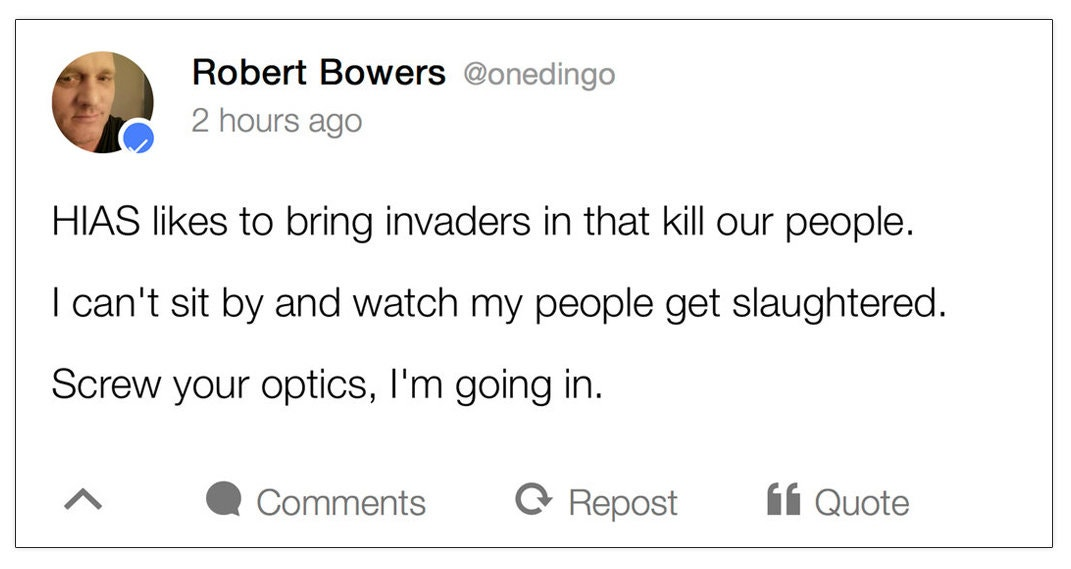
\includegraphics[height=6cm, keepaspectratio]{img/gab-pittsburgh-post.jpg}
    \caption{Último post de Robert Bowers, tirador en la masacre de Pittsburgh, en la red social Gab.}
    \label{fig:gab_post}
\end{figure}


En Octubre de 2018, un hombre fuertemente armado entró a la sinagoga ``El Árbol de la Vida'' en Pittsburgh, Pensilvania, Estados Unidos. Luego de gritar ``muerte a los judíos'', abrió fuego contra la multitud matando 11 personas y dejando decenas de heridos, la matanza más grande de judíos en EEUU de la que se tenga registro.

El tirador, Richard Bowers, era usuario activo de Gab \footnote{\url{https://gab.com/}}, una red social que nació en 2016 bajo la égida de la defensa de la ``libertad de expresión'' a raíz de la creciente moderación de Twitter y Facebook a discursos discriminatorios. Desde entonces, ha sido el refugio de activistas de la derecha alternativa, supremacistas raciales, grupos conspiracionistas y otros elementos reaccionarios. El asesino en cuestión posteaba frecuentemente contenido antisemita en dicha red social \cite{mcilroy2019welcome}, particularmente contra la HIAS (Sociedad Hebrea de auxilio de inmigrantes). En su último post en dicha red social, horas antes de la masacre, Bowers posteó una amenaza (ver figura \ref{fig:gab_post}) diciendo que no podía tolerar ver a su gente ser asesinada (por judíos) y que iba a tomar acciones al respecto.

A raíz de esto, Gab --llamada popularmente como el ``Twitter racista''-- estuvo de baja durante cierto tiempo al serle negado alojamiento web debido a este atentado. Desde entonces, diversos trabajos han recopilado y analizado el contenido discriminatorio en esta red social \cite{mcilroy2019welcome,kennedy2018gab}.



\subsection{Masacre Rohingya en Myanmar}
% https://www.quigsclass.com/uploads/7/2/6/8/72681355/5_myanmar_facebook.pdf
%
Entre 2016 y 2017 fue perpetrada una matanza de la etnia Rohingya, un grupo étnico musulmán, en la República de Myanmar (ex Birmania). Cerca de 25 mil personas fueron masacradas y un éxodo de más de 700 mil personas tuvo lugar hacia la lindante Bangladesh, conformando el campamento de refugiados más grande del mundo en la actualidad. La ONU y algunos estados nacionales han calificado lo ocurrido como un ``genocidio'' y como una ``limpieza étnica''.


Si bien el sometimiento de este pueblo tiene lugar hace décadas, en los últimos años tuvo un gran recrudecimiento motorizado desde las altas esferas gubernamentales y militares birmanas, que niegan cualquier estatus legal a la población rohingya. En ese punto, las redes sociales han jugado un rol de difusor y catalizador de incitaciones a la violencia y noticias falsas alrededor de esta etnia. Según un informe solicitado por Facebook acerca de la situación en Myanmar \cite{warofka2018independent}, gran parte de este problema se debe a un déficit en el ``alfabetismo digital''(sic) de la población de este país, que usa casi exclusivamente Internet a través de dicha red social. Enviados de las Naciones Unidas han acusado directamente a Facebook de haber servido como intermediario de discurso de odio a través de su plataforma \footnote{\url{https://www.reuters.com/article/us-myanmar-rohingya-facebook/u-n-investigators-cite-facebook-role-in-myanmar-crisis-idUKKCN1GO2PN}}, y que ha tenido un ``rol determinante'' en este genocidio.

Organizaciones de derechos humanos de ese país han instado a la empresa de Mark Zuckerberg a invertir en el control del discurso de odio, particularmente aquel que insta a la violencia física \cite{irrawaddy2018zuckerberg}. A finales de 2021, un grupo de refugiados rohingya denunció a Facebook por 150 mil millones de dólares \footnote{\url{https://www.bbc.com/news/world-asia-59558090}} por haber promovido la violencia contra esta etnia, luego de que en 2018 responsables de la empresa admitieran que no se hizo lo suficiente para detener la proliferación del discurso xenófobo contra los Rohingya en Myanmar.

Este hecho cuenta con una particularidad: apunta a un idioma --el birmano, idioma oficial en Myanmar-- que dispone de pocos recursos en el área del procesamiento del lenguaje natural. La mayoría de los recursos y estudios están dedicados al idioma inglés, ignorando las particularidades de cada idioma y el componente cultural de algunas tareas, como en este caso la detección de discurso de odio. Además, según Reuters, para finales de 2018 Facebook no contaba con ningún empleado en Myanmar \footnote{\url{https://www.reuters.com/investigates/special-report/myanmar-facebook-hate/}} ni tampoco quedaba claro que alguno de sus empleados dedicados a la tarea del monitoreo sea hablante nativo de birmano.


\section{Avances en el procesamiento del lenguaje natural}

En los últimos 10 años, el área de la Inteligencia Artificial ha sido sacudida por la irrupción de las redes neuronales. Desde el campo de Visión por Computadora, un conjunto de factores han potenciado el éxito de esta técnica de aprendizaje estadístico: datasets de gran tamaño como ImageNet \cite{imagenet2009deng}, la utilización de dispositivos de gran poder de cómputo como las GPUs, y el desarrollo de mejores algoritmos para su entrenamiento (de optimización, funciones de activación, entre otras cosas). Esta combinación posibilitó que las redes neuronales obtengan mejoras considerables en el desempeño de tareas de reconocimiento de imágenes, trasladándose esto a otras áreas como procesamiento de habla, y a todas las áreas de aprendizaje automático en general, con particular foco de aquellos datos no estructurados como imágenes, sonido, y otras señales.

Este boom inicial tuvo su primera repercusión de magnitud en NLP cerca del año 2013 con el desarrollo de los word-embeddings. La técnica de \emph{word2vec} \cite{mikolov2013distributed} permitió generar representaciones de palabras de manera eficiente sobre grandes cantidades de datos no etiquetados. Estas representaciones de las palabras (podemos pensarlas como vectores de dimensión fija asignadas a cada token) han sido la ``salsa secreta'' que permitió el éxito de las redes neuronales en el área, permitiendo una mejora en las tareas de reconocimiento de entidades nombradas (NER), POS tagging, parsing, clasificación de textos, entre otras. Otro componente de este éxito de las redes neuronales ha sido el uso de redes recurrentes como las Long Short-Term Memory (LSTM) \cite{hochreiter1997long} o las Gated Recurrent Units (GRU) \cite{cho-etal-2014-learning}, que permiten codificar secuencias de manera autorregresiva. Un caso de éxito particular utilizando estas redes recurrentes ha sido el de la traducción automática mediante la arquitectura sequence-to-sequence (seq2seq) \cite{sutskever2014sequence}. Estas redes permitieron atacar los problemas de aprendizaje de secuencia a secuencia, como la traducción automática o resumen automático de texto, reemplazando sistemas realmente complejos y de difícil mantenimiento (como los de Statistical Machine Translation) por diseños más simples y con una muy superior performance.

En 2017, \citet{vaswani2017attention} propusieron una arquitectura que elimina la estructura recurrente: los \emph{Transformers}. Este modelo utiliza únicamente múltiples capas de auto-atención para el problema de traducción automática. Al eliminar los pasos recurrentes, permitió la paralelización del cálculo y el entrenamiento de arquitecturas verdaderamente profundas para tareas de NLP, como ya hace tiempo se utilizaban en el área de Visión por Computadora. En conjunto a la aplicación del pre-entrenamiento utilizando la tarea de modelado de lenguaje (que introdujeron \citet{howard-ruder-2018-universal} con ULMFiT, entre otros trabajos) supusieron un cambio rotundo en el modo en que abordamos tareas de aprendizaje automático sobre textos: en lugar de entrenar una red neuronal casi desde cero --quizás sólo con una capa de embeddings con pesos iniciales pre-calculados-- la idea es ahora sólo ajustar (\emph{fine-tune}) una gran red neuronal pre-entrenada sobre un dataset de entrenamiento con alguna tarea de modelado de lenguaje. \emph{GPT}, \bert{} y otros personajes de Plaza Sésamo son algunos de los rutilantes nombres en el zoológico de modelos pre-entrenados que son hoy día el estado del arte de NLP. Este nuevo enfoque supuso un gran paso adelante en el área, mejorando los desempeños sensiblemente en benchmarks de tareas como GLUE \cite{wang-etal-2018-glue} y RACE \cite{lai2017race}, entre otros.

En suma, todos estos avances han permitido atacar numerosas tareas que eran problemáticas para NLP. Algunas --como resumen o traducción automática-- que adolecían de pobres performances o sistemas realmente complejos y difíciles de mantener. Otras, que simplemente estaban fuera del radar del estado del arte, como por ejemplo tareas de Common Sense Reasoning \todo{citar ejemplos de esto}. Dentro de estas tareas, ĺa detección de discurso de odio y toxicidad ha sido de aquellas tareas que, si bien en la etapa previa han podido utilizar sistemas basados en la detección de n-gramas, eran muy frágiles y susceptibles ante el ruido típico de este tipo de texto. Con el advenimiento de modelos neuronales y representaciones más robustas, han mejorado notablemente su performance frente a escenarios más complejos. A su vez, nuevas tareas han sido propuestas para lidiar con este fenómeno, como la respuesta automática a mensajes discriminatorios   \todo{A esto le falta un poquito de desarrollo}

\subsection{Asimetría de recursos}

Un problema no menor en el área de NLP es la enorme asimetría de recursos entre idiomas. La inmensa mayoría de datasets, corpus, modelos y --consecuentemente-- estudios han sido realizados en inglés. En particular, el caso de los modelos pre-entrenados basados en Transformers introducidos en los últimos años vienen a agravar esta asimetría ya que estos modelos necesitan muchos recursos computacionales para ser generados, usualmente no disponibles por fuera de algunos pocos laboratorios que centran sus estudios en inglés. Esto ocasiona, por un lado, la creencia generalizada de que muchas técnicas son \emph{independientes del lenguaje}, omitiendo importantes diferencias entre lenguajes y dialectos. Por otro lado, teniendo en cuenta que el objeto de este trabajo es mayormente sociolingüístico, esto dificulta la posibilidad de realizar estudios posteriores utilizando los recursos generados en forma de modelos o datasets.

Para atacar este problema, es entonces necesario desarrollar recursos y estudios en los distintos idiomas, atendiendo sus particularidades lingüísticas y culturales. La ``Regla de Bender'' describe de manera elegante esto:

\begin{displayquote}[Regla de Bender, \citet{bender2011achieving}]
    Do state the name of the language that is being studied, even if it's English. Acknowledging that we are working on a particular language foregrounds the possibility that the techniques may in fact be language specific. Conversely, neglecting to state that the particular data used were in, say, English, gives a false veneer of language-independence to the work.
\end{displayquote}

Si bien el español puede considerarse de los idiomas dentro del grupo de los de ``altos recursos'' \cite{bender2019rule}, aún así la disparidad al compararse con el inglés es abrumadora. En particular, para el área de interés de esta tesis --la detección de discurso de odio--, los recursos son muy escasos y, en la mayoría de los casos, ``réplicas'' de trabajos hechos en inglés, sin ninguna novedad adicional.

\section{Detección de discurso de odio y sus limitaciones}

%
%
% https://docs.google.com/drawings/d/1wy148WBa5f6FcHco9j9u_Xy8LUrmkREL136JVNOea6Y/edit
%
%

\begin{figure}
    \centering
    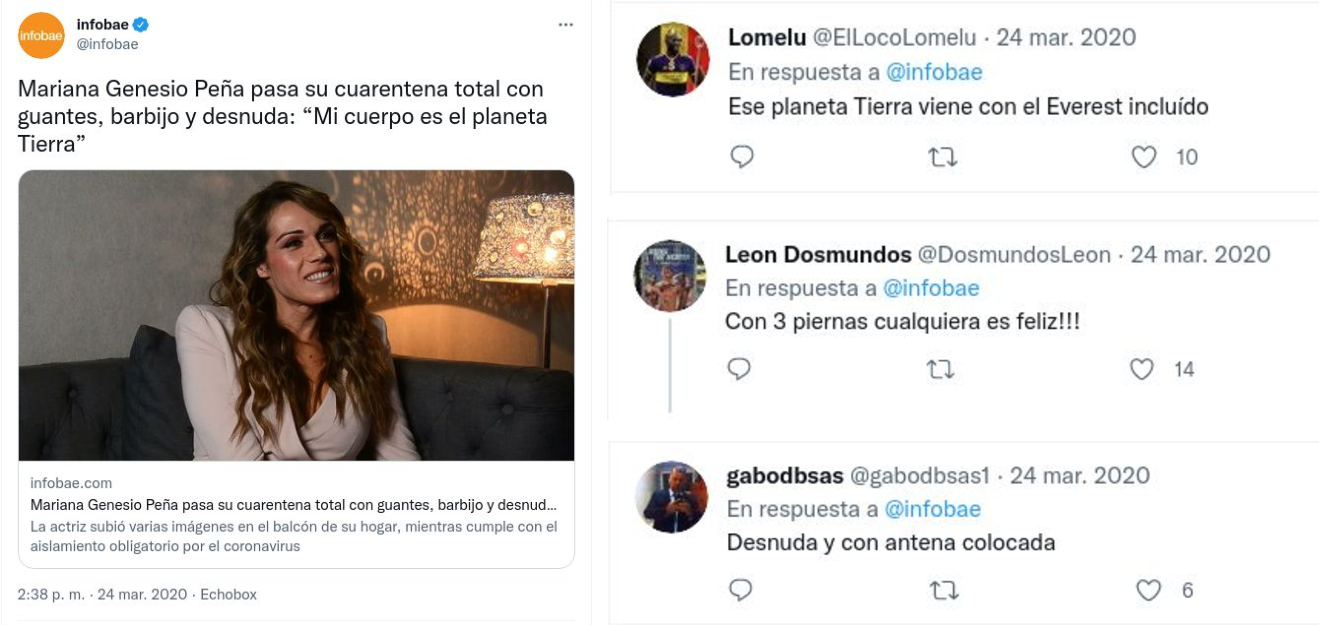
\includegraphics[width=\textwidth]{img/01/tweets_contexto.pdf}
    \caption{Tweets y respuestas discriminatorias. Leyendo únicamente el texto de los comentarios resulta difícil descifrar su sentido. }
    \label{fig:01_tweets_y_su_contexto}
\end{figure}

Como dijimos anteriormente, la detección del discurso de odio puede pensarse como una tarea de clasificación binaria sobre un texto generado por un usuario. Muchos trabajos en los últimos años han abordado la tarea desde esa perspectiva, desarrollándose numerosos recursos en workshops para varios idiomas, y herramientas muy utilizadas para la moderación de contenido tóxico \footnote{El contenido tóxico o abusivo es una categoría un poco más general que la de discurso de odio} como Perspective API \footnote{\url{https://www.perspectiveapi.com/}}, desarrollada por Jigsaw y Google.

Si bien predecir únicamente si un comentario contiene o no lenguaje discriminatorio tiene una innegable utilidad, este enfoque adolece de ciertas limitaciones. Uno de sus problemas es la falta de contexto en los mensajes analizados. Las personas no solemos consumir el lenguaje de manera aislada sino que lo entendemos situado de acuerdo a varios factores: el emisor, la situación y el medio en el que se lo emite, a quién está dirigido, sobre qué hace mención, entre otras cosas. La mayoría de los estudios y recursos, sin embargo, están realizados sobre datos fuera de contexto: mensajes en redes sociales sin ningún tipo de información conversacional o de otra índole. Para ilustrar el problema de la falta de contexto, la figura \ref{fig:01_tweets_y_su_contexto} muestra un tweet de un medio periodístico que habla sobre una actriz y respuestas a esa noticia \footnote{El hilo completo puede encontrarse en \url{https://twitter.com/infobae/status/1242506130213015552}}. Leyendo los tweets por fuera del contexto es difícil comprender las respuestas con contenido transfóbico dirigidos a la actriz en cuestión.

La falta de contexto restringe la información disponible --tanto para un humano como para un algoritmo-- para poder discernir si un comentario de un usuario es o no discriminatorio. Otra información usualmente no disponible y que puede ayudar a enriquecer la detección de discurso de odio es la característica atacada en un texto: es común que los datasets estén anotados de manera poco granular --casi siempre de manera binaria-- no brindando información acerca de si la agresión es por motivos de género, religión, etnia, etc. Contar con esta información puede ser de utilidad para que un algoritmo pueda detectar mejor los diferentes tipos de discurso discriminatorio mediante una señal más rica. Así también, los usuarios de estos algoritmos de detección automática de discurso de odio podrían obtener información más concreta acerca del fenómeno detectado: no sólo si es discriminatorio o no sino el motivo por el cual se lo considera.

Por último, una limitación puntual del español es la poca disponibilidad de recursos para esta tarea, algo que mencionamos en la anterior sección como un problema general de NLP. A esto se le suma que los pocos datasets disponibles --tanto para español como otros idiomas-- suelen adolecer de cierto déficit de calidad en su construcción: generados por equipos con poca o nula interdisciplina; o bien anotados por sujetos que no son hablantes nativos del idioma en cuestión o no están inmersos en su realidad sociocultural.

\section{Aportes de este trabajo}

En esta tesis nos proponemos hacer un aporte en el sentido de desarrollar mejores mecanismos automáticos de detección de discurso de odio. Si bien el área de NLP ha avanzado enormemente en los últimos años -- y esta subdisciplina en particular ha recibido un gran interés-- creemos que muchos de los enfoques actuales inhiben un avance cualitativo en la detección de este pernicioso fenómeno en medios sociales.

Para ello, en primer lugar estudiamos técnicas de detección sobre recursos ya existentes, utilizando del estado del arte. En base a la observación de algunos datasets y la literatura en general, planteamos un nuevo problema: la detección \emph{contextualizada} de discurso de odio. Construimos un corpus de discurso de odio sobre comentarios en noticias de medios gráficos argentinos en \twitter{}, siendo este conjunto de datos etiquetado por hablantes nativos. Este dataset es un aporte importante en sí ya que es uno de los primeros que incluyen información contextual, y es el único a nuestro conocimiento en español que tiene esta información. A su vez, fue construido de manera interdisciplinaria y con una metodología clara en su recolección y anotación.

Con este recurso, exploramos la siguiente pregunta: ¿pueden los métodos actuales basados en modelos pre-entrenados aprovechar información adicional de contexto para mejorar la detección de discurso de odio? Este punto ha sido poco estudiado en la literatura y consideramos que es una pregunta de interés para atravesar los límites de la clasificación basada en una única fuente de información (el comentario analizado). En base a los experimentos realizados, encontramos evidencia de que el contexto puede brindar información útil para detectar este fenómeno, mejorando el desempeño de los algoritmos para esta tarea. Particularmente, observamos que para los mensajes de odio contra ciertos grupos --por ejemplo, contra la comunidad LGBTI-- el contexto puede ser aún más útil para su detección.

Finalmente, realizamos un estudio más en general sobre la \emph{adaptación de dominio} en tareas de clasificación de redes sociales. Para ello, generamos un modelo de lenguaje pre-entrenado sobre textos sociales en español al que bautizamos \robertuito{}, el primero disponible y a gran escala en este idioma. Comparamos el desempeño de \robertuito{} contra otros pre-entrenados sobre textos formales pero ajustados al dominio social. Esta comparación es de interés ya que el ajuste de dominio es relativamente económico frente al enorme costo de entrenamiento que tiene construir modelos como \robertuito{}. Observamos que para todas las tareas, \robertuito{} obtiene una performance del estado del arte, pero el ajuste de dominio recorta considerablemente la brecha contra otros modelos.

Un aporte en general de esta tesis es que todos los estudios y recursos han sido realizados en español. Vista la enorme asimetría que hay con otros idiomas, y teniendo en cuenta que el español es el segundo idioma en hablantes nativos del mundo, consideramos necesario mitigar este desbalance de recursos.


\chapter{Preliminares}
En esta sección haremos una breve introducción a algunas técnicas de Machine Learning y NLP que utilizamos a lo largo de esta tesis. Particularmente, ilustraremos y describiremos a grandes rasgos los últimos avances de Deep Learning para el área, desde \emph{word2vec} \cite{mikolov2013distributed} hasta la arquitectura Transformers \cite{vaswani2017attention}.

\section{Aprendizaje supervisado}

Muchas de las tareas de las áreas de Procesamiento de Lenguaje Natural, Visión por Computadora, Procesamiento del Habla (entre otras) pueden convertirse a problemas de aproximar una función $f: D \rightarrow O$, donde $D$ es el \emph{dominio} y $O$ el codominio o posibles salidas. Las funciones que es de nuestro interés aproximar son desconocidas, altamente no lineales y muy complejas. En el caso de que $O$ sea un conjunto finito, diremos que estamos ante un problema de \textbf{clasificación} y llamaremos a nuestro aproximador $\widehat{f}$ \textbf{clasificador} y a cada uno de las posibles salidas \textbf{clases}. En el caso de que $O$ conste de una o más variables continuas, decimos que estamos ante un caso de \textbf{regresión}. Para lo que concierne a esta tesis, nos centraremos en problemas de clasificación, así que restringiremos (salvo en los lugares donde se explicite lo contrario) nuestro análisis a este tipo de tareas.

Un ejemplo canónico de clasificación del área de Visión por Computadora es el de, dada una imagen de 28 x 28 píxeles en blanco y negro, predecir a cual de los 10 caracteres pertenece. En este caso, tenemos que $D$ es un subconjunto de ${0, 1}^{28 \times 28}$ --todas las imágenes posibles de ese tamaño en blanco y negro-- restringido a aquellas imágenes que correspondan a caracteres, y que $O = {0, 1, 2, \ldots, 8, 9}$ son las posibles salidas de esta función.

En el caso de NLP, uno de los que problemas que más veremos en esta tesis es el de clasificación de textos: dado un texto (un documento, un comentario en una red social) predecir alguna característica discreta de éste. Por ejemplo, si el texto es un comentario de una red social, podemos intentar identificar su polaridad: si es positivo, neutro, o negativo. O si el comentario en cuestión posee algún tipo de discriminación: en este caso tenemos como posibles salidas 0 (marcando no discriminatorio) o 1 en caso de que sí haya discriminación. Otro tipo de tarea es la de inferencia (Natural Language Inference o NLI): dadas dos oraciones de texto, predecir si una es una consecuencia lógica de la otra, si son independientes, o si son contradictorias. En este caso, el dominio son pares de oraciones de texto, y tenemos tres posibles salidas: contradicción, independiente, consecuencia.

Estos problemas que acabamos de describir son realmente difíciles de atacar mediante programas convencionales diseñados a través de heurísticas o reglas prefijadas \cite{bishop2006pattern}. En lugar de ello, los abordaremos mediante técnicas de \textbf{aprendizaje supervisado}, en el cual tendremos un conjunto de instancias $x_1, \ldots, x_n$ y sus respectivas etiquetas $y_1, \ldots , y_n$ que usaremos para entrenar nuestro aproximador $y \sim f^*(x)$. Este conjunto $\{ (x_1, y_1), \ldots (x_n, y_n)\}$ se denomina \textbf{conjunto de entrenamiento}.

El proceso de entrenamiento de un estimador consta de seleccionar una función $f\theta$ de un conjunto de candidatos $\{f_\theta: \theta \in \Sigma\}$, donde $\theta$ representa los parámetros del clasificador, y $\Sigma$ representa el conjunto de sus posibles valores. En el caso de un clasificador lineal (como una Support Vector Machine o una regresión logística) $\theta$ constará de un vector de $\mathbb{R}^n$. En el caso de redes neuronales (como las que veremos a continuación), constará de múltiples matrices y vectores correspondientes a sus diferentes capas.

\todo{Mencionar otras tareas que no estén mencionadas: transducción de secuencias, modelado de lenguaje}

Si bien en algunos capítulos de esta tesis utilizamos técnicas de clasificación lineal como Support Vector Machines y regresiones logísticas, nuestro eje está puesto en los modelos basados en redes neuronales. Estos modelos han logrado el estado del arte en NLP para casi cualquier tarea conocida, y pasamos a continuación a hacer un repaso de sus distintas variantes. Para una descripción de los modelos lineales, referimos a textos clásicos del área como \citet{bishop2006pattern}.

\section{Redes Neuronales}


Los \tbf{perceptrones multi-capa} (MLP) o \tbf{redes feed-forward} (FFN) son la ``quintaesencia'' de los métodos modernos de Deep Learning, como describen \citet{goodfellow2016deep}. Una de las primeros acercamientos a esta técnica es la neurona de McCulloch-Pitts \cite{mcculloch1943logical}, que intenta modelar parte del funcionamiento de las neuronas mediante una función:

\begin{equation*}
    y = H(\theta^T x)
\end{equation*}

\noindent donde $H$ es la función de Heaviside o función escalón, que vale $1$ si $x \geq 0$, y $0$ en otro caso. La neurona de McCulloch-Pitts permite aproximar a dos valores (0 ó 1), a partir de una entrada $x$ y un parámetro $\theta$. El perceptrón, desarrollado en 1958 en \citet{rosenblatt1958perceptron}, es el primer modelo que utiliza este tipo de modelo de cómputo cuyos parámetros se encuentran mediante un algoritmo. \citet{minsky1969perceptrons} demostraron que este tipo de modelos sólo pueden ajustarse a datos linealmente separables, provocando que por largo tiempo no se profundice en la investigación de redes neuronales.

Una forma de sortear estas dificultades planteadas es apilar (stack) estas neuronas para poder ajustar a más tipos de funciones. En términos matemáticos, esto es tan sólo una composición de funciones, tomando ahora $f = f_3 \circ f_2 \circ f_1$, donde $f_1$ es la primer ``capa'' de nuestra función correspondiente a la entrada, $f_2$ es la capa intermedia u oculta, y $f_3$ es la capa de salida, cada una teniendo sus parámetros $\theta_1, \theta_2, \theta_3$. Si bien este ejemplo consta de 3 capas, se puede generalizar a arbitrarias capas ocultas. Este modelo es el que conocemos como \textbf{Perceptrón Multicapa} o \textbf{Multi-Layer Perceptron} (MLP por sus siglas en inglés), y provocó el resurgir conexionista de las redes neuronales en los años 80s gracias al desarrollo de algoritmos que permitieron entrenar estos modelos mediante la técnica de backpropagation \cite{rumelhart1986learning}.

\citet{cybenko1989approximation} demostró que para cualquier función continua en el hipercubo de $\mathbb{R}^n$ existe una red neuronal con una función de activación sigmoidal de 3 capas que la puede aproximar infinitamente bien \footnote{La formulación del resultado es un poco más compleja pero escapa los fines de esta tesis}. Sucesivos resultados demostraron con mayor generalidad este resultado, para otras funciones de activación (como las ReLU) y otras arquitecturas. Dicho en términos coloquiales, este teorema asegura que para cualquier función podemos encontrar una MLP que la aproxima. Hay que notar, sin embargo, que estos teoremas aseguran existencia pero no son constructivos, y tampoco aseguran que el proceso de backpropagation nos lleve a esa solución \cite{goodfellow2016deep}. Tampoco nos dice qué tan grande tiene que ser la red neuronal para que pueda aproximar adecuadamente a la función objetivo. Teniendo estas salvedades en cuenta, estos teoremas (usualmente denominados como Teorema de Aproximación Universal de Redes Neuronales) aportan un sustento teórico de la potencialidad de estos algoritmos, refutando en cierto punto lo marcado por \citet{minsky1969perceptrons}.

\subsection{Redes neuronales recurrentes}

\begin{figure}
    \centering
    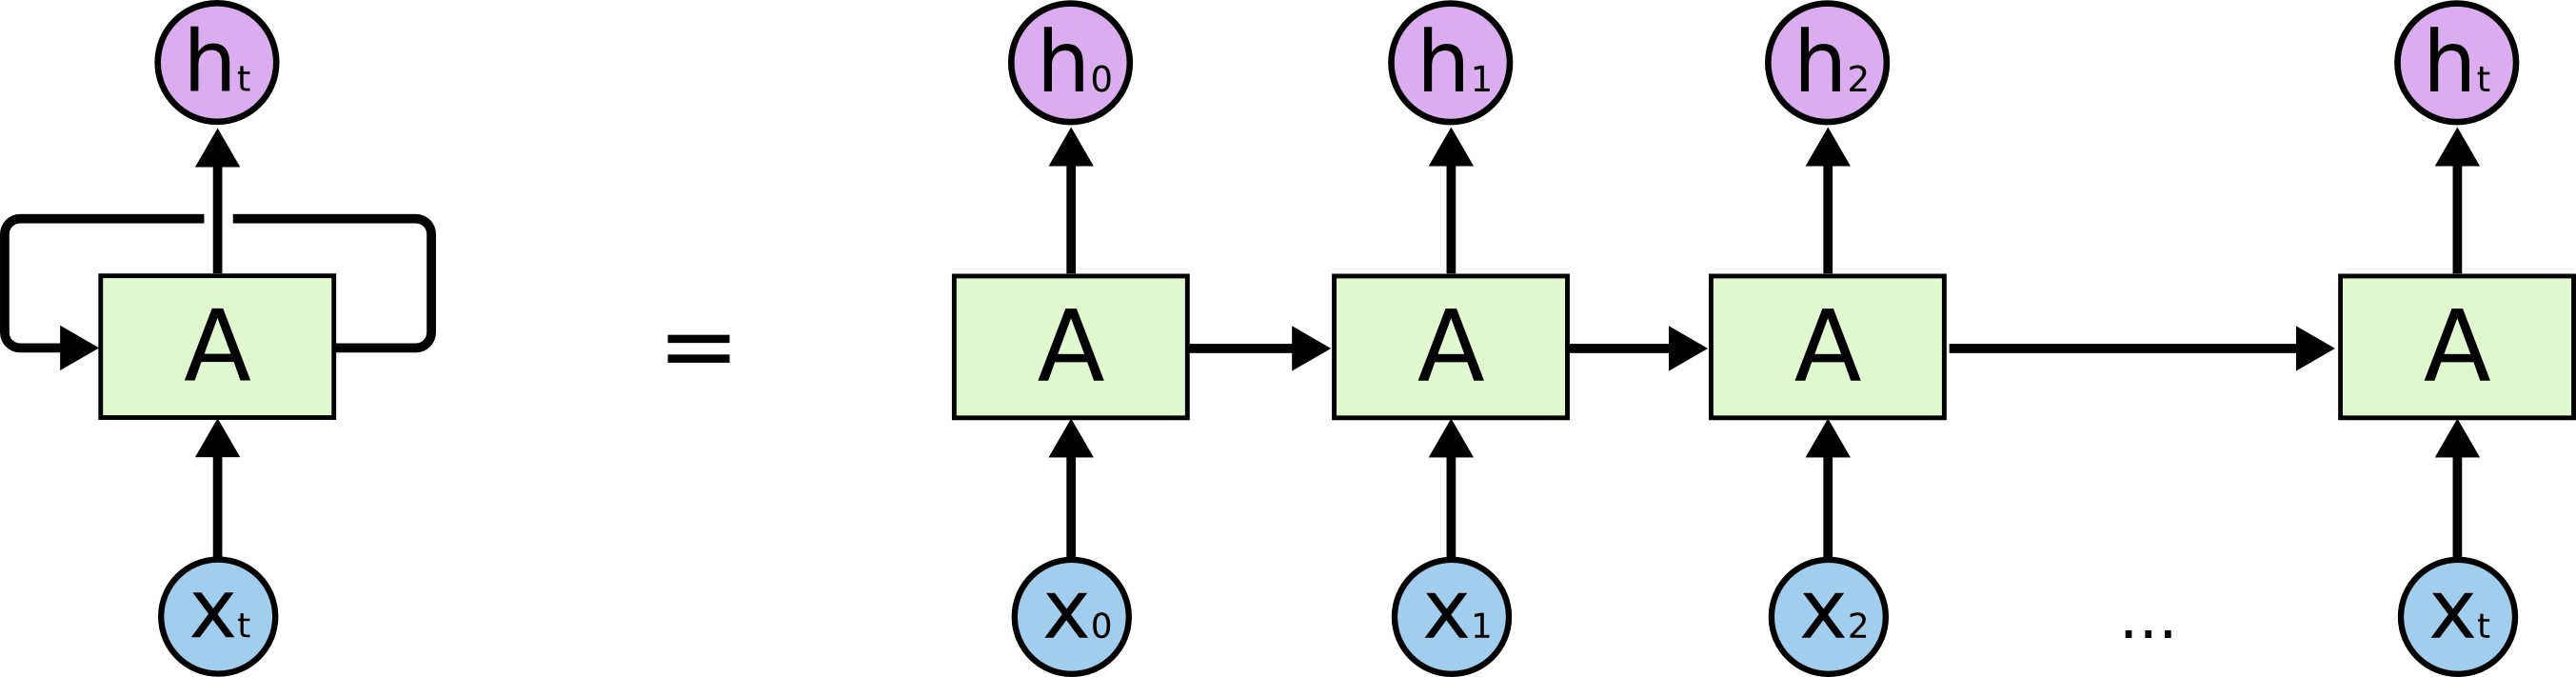
\includegraphics[width=0.8\textwidth]{img/rnn.png}
    \caption{Ilustración del esquema general de una red neuronal recurrente. Fuente: Blog de Christopher Olah}
    \label{fig:recurrent_net}
\end{figure}

Los problemas descriptos de NLP suelen constar de procesar una secuencia de palabras o tokens $x_1, x_2, \ldots, x_k$ de longitud variable, de manera de ajustar a una función

\begin{equation*}
    h = f([x_1, \ldots, x_k])
\end{equation*}

Una reformulación de este problema convirtiéndolo a una función que recibe una entrada de largo fijo es el de ajustar una función autorregresiva:

\begin{equation*}
    h_t = f(x_t, h_{t-1})
\end{equation*}

\noindent En este caso, tenemos una salida para cada paso $k$ de tiempo. Si $f$ es una red neuronal, llamamos a este tipo de redes neuronales \textbf{recurrentes}, ya que la salida a cada paso ($h_t$) depende de la salida del paso anterior, $h_{t-1}$. La figura \ref{fig:recurrent_net}  ilustra este esquema, tomada del excelente artículo de Chirstopher Olah sobre LSTMs \footnote{\url{https://colah.github.io/posts/2015-08-Understanding-LSTMs/}}. Una primer aproximación a las redes recurrentes es la red de Elman \cite{elman1990finding}, definida por las siguientes ecuaciones

\begin{align}
h_t &= \sigma(W_h x_t + U_h h_{t-1} + b_h) \\
y_t &= \sigma(W_y h_t + b_y)
\label{eq:elman}
\end{align}

\noindent donde $h_t$ es normalmente llamado el \textbf{estado oculto} en las redes neuronales recurrentes, e $y_t$ es la salida propiamente dicha. Los parámetros a ajustar son $W_h, U_h$ (matrices) y $b_h, b_y$ (escalares). Podemos ver que, a grandes rasgos, este tipo de red recurrente no es nada más que un perceptrón multicapa cuya entrada consta de $x_t$, la entrada original en el tiempo actual $t$, y el estado oculto anterior, $h_{t-1}$.

Para entrenar este tipo de redes recurrentes utilizamos back-propagation through time (BPTT), que consta en desplegar la relación recurrente --como está ilustrado en la figura \ref{fig:recurrent_net}-- y aplicar back-propagation de manera normal, poniendo un límite en la cantidad de pasos que tomamos hacia atrás. Las redes recurrentes de Elman sufren de varios problemas, principalmente de \textbf{vanishing gradient} y \textbf{exploding gradient}. Ambas dificultades pueden observarse ya que el cálculo del gradiente de las ecuaciones \ref{eq:elman} usando BPTT induce la potencia a la $n$ (donde $n$ es el largo de la secuencia) de las matrices $W_h$ y $U_h$, lo cual puede hacer o que bien el gradiente tienda a cero o a infinito. \footnote{ Esto puede verse usando alguna descomposición de la matriz como la forma normal de Jordan. Sus elementos en la diagonal que sean distintos de 1, o bien tienden a infinito o a cero.}

Los gradientes que tienden a infinito o \textbf{exploding gradient} pueden solucionarse mediante la técnica de \textbf{gradient clipping} \cite{goodfellow2016deep}, que consta de reajustar la norma del gradiente para que no exceda cierto valor. Sin embargo, nos queda aún el inconveniente de vanishing gradient. Para ello, se han propuesto otras arquitecturas recurrentes. \citet{hochreiter1997long} propusieron las \textbf{Long Short-Term Memory} (LSTM), una arquitectura basadas en compuertas (gates) que regulan el comportamiento del estado oculto y de la salida, evitando algunos de las dificultades de aprendizaje en las que incurre la red de Elman \footnote{Recomendamos el artículo antes mencionado de Christopher Olah para una muy buena explicación de este tipo de redes}. Otras arquitecturas como las Gated Recurrent Units \cite{cho-etal-2014-learning} usan menor cantidad de compuertas reduciendo la cantidad de parámetros a entrenar.

\section{Técnicas de representación}
\label{sec:02_representaciones}

Una de las necesidades que tienen las redes neuronales para poder trabajar con textos es el de tener representaciones continuas de cada token o palabra. Las representaciones utilizadas en la época previa de los donde reinaban los modelos lineales --bolsas de palabras/caracteres ponderadas con esquemas como TF/IDF-- adolecen de varios inconvenientes. En primer lugar, tienen una altísima dimensionalidad, usualmente del tamaño del vocabulario o algún límite similar. A su vez, no guardan representación semántica de la similaridad de las palabras: dos palabras como silla o banco tienen la misma distancia que perro y nube. Finalmente, sus valores no nulos están concentradas en una o pocas dimensiones y suelen ser discretas.

Latent Semantic Analysis (LSA) \cite{landauer1997solution} es una de las primeras técnicas de representación continua que tuvo cierta popularidad. Para obtener representaciones continuas de las palabras, plantean la factorización una matriz de co-ocurrencia entre tokens y documentos (o contextos) usando la descomposición SVD, obteniendo vectores de dimensión fija para los documentos y términos. LDA (Latent Dirichlet Allocation) \cite{blei2003latent} es otra técnica basada en modelos gráficos entrenados mediante métodos variacionales, muy utilizada aún en la actualidad ya que genera representaciones latentes de los tópicos de los textos.

%\begin{figure}
%    \centering
%    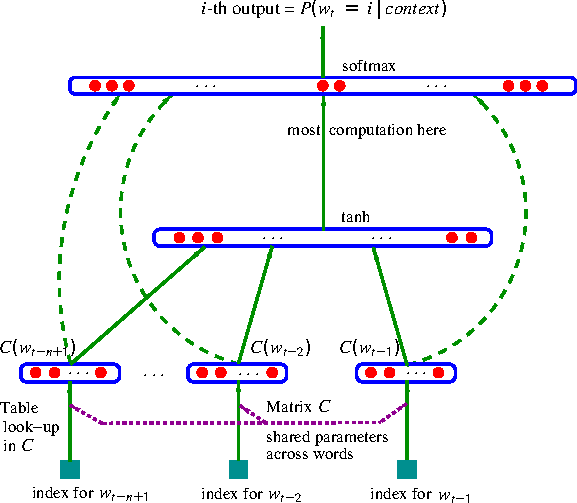
\includegraphics[width=0.65\textwidth]{img/02/bengio_neural_language_model.pdf}
%    \caption{Ilustración del modelo de lenguaje neuronal de \citet{bengio2003neural}. La entrada consta de $n-1$ palabras, que primero pasan por una lookup table (o capa de embeddings), una función de activación y son colapsadas para luego ser utilizadas como entrada de una función softmax.}
%    \label{fig:bengio_neural_language_model}
%
%\end{figure}

Dentro de los métodos neuronales, uno de los más populares ha sido el de \citet{bengio2003neural}, que propone una arquitectura neuronal para un modelo de lenguaje markoviano. %La arquitectura de esta red está ilustrada en la figura \ref{fig:bengio_neural_language_model}%.
En la capa intermedia contiene una tabla de lookup de vectores de las diferentes palabras (también conocido como capa de embeddings) donde se generan las representaciones de las palabras durante la etapa de entrenamiento. Trabajos posteriores (con diferentes variaciones de esta misma idea) como el de \citet{collobert2011natural} han demostrado que la utilización de este tipo de representaciones es útil para diversas tareas de NLP como POS Tagging, NER, y otras. Más aún, este trabajo tiene una idea que fue utilizada muchos años después con éxito rotundo: la utilización de la tarea de modelado de lenguaje como base para el pre-entrenamiendo de redes neuronales.

Uno de los problemas de los métodos comentados es que no son muy eficientes, sólo pudiéndose entrenar con pocos millones de palabras y con dimensiones reducidas. La técnica \emph{word2vec} \cite{mikolov2013efficient} permite entrenar representaciones de mayor dimensión y sobre grandes cantidades de textos de manera eficiente. Los vectores de palabras aprendidos guardan cierta estructura lineal y semántica, ilustrado por los autores con algunos ejemplos de analogías de palabras como el ya clásico $v(\text{rey}) - v(\text{hombre}) + v(\text{mujer}) \approx v(\text{reina})$.

Para generar los vectores de \emph{word2vec}, los autores plantean una relajación de la tarea de modelado de lenguaje mediante dos alternativas: Continuous Bag of Words (CBOW) y Skip-Gram. En CBOW se intenta predecir la palabra faltante dada una bolsa de palabras del contexto, mientras que Skip-gram se intenta predecir el contexto dada la palabra central, obteniendo en ambas variantes representaciones intermedias ricas. \citet{mikolov2013efficient} extiende la idea del anterior trabajo proponiendo plantear el problema de skip-gram como uno de distinguir palabras ruido de palabras efectivamente del contexto, haciendo mucho más eficiente el cálculo de estas representaciones. \emph{GloVe} \cite{pennington2014glove} es otra técnica de representación de palabras que combina las ideas de factorización de matrices de LSA  mediante un problema de optimización distinto y generando representaciones que superan ligeramente en algunos benchmarks de tareas a los de \emph{word2vec}.

Los métodos mencionados de representación calculan vectores de tamaño fijo sobre cada una de las distintas palabras. En español, por ejemplo, las palabras gato, gata, gatito, gatuno, todas tienen representaciones independientes en \emph{word2vec}, a pesar de tener información morfológica en común. Esto es un problema en varios escenarios: idiomas con muchas inflexiones o aglutinantes (como el turco, alemán o finés) o --lo que es de nuestro interés-- texto altamente desnormalizado como el de redes sociales. La técnica \fasttext{} \cite{bojanowski16} extiende la idea de \emph{word2vec} mediante la asignación de vectores a secuencias de 3 caracteres (subpalabras), capturando así cierta información morfológica. La representación de una palabra se obtiene mediante una combinación lineal de los vectores de las subpalabras que la componen.

\subsection{Embeddings a nivel oración}
\label{sec:02_tweet_embeddings}

%%
%%
%%
%%  https://docs.google.com/drawings/d/1BU3ulBiqU0NojpW6Fkb4xFlMCDigSWwfjN7z9smO6nY/edit
%%
%%

\begin{figure}[t]
    \centering
    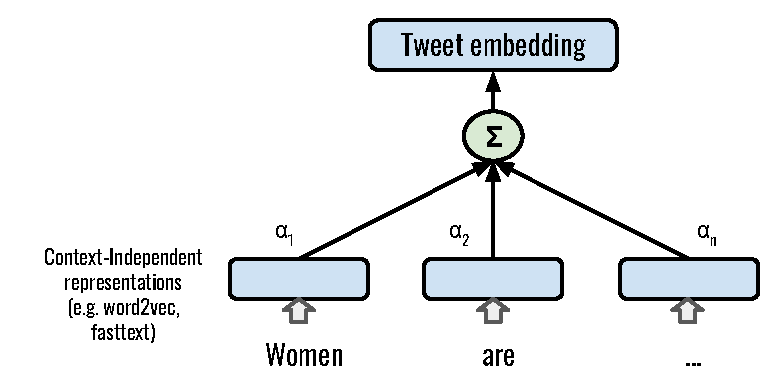
\includegraphics[width=0.75\textwidth]{img/tweet_embeddings.pdf}
    \caption{Representación continua de un tweet mediante combinación lineal de las representaciones de cada palabra.}
    \label{fig:tweet_embeddings}
\end{figure}

Una forma relativamente simple de obtener una representación de un texto \footnote{en nuestra tesis, esto será casi siempre un tweet} es realizar una combinación lineal de las representaciones obtenidas para cada palabra. Es decir, dada una oración $s = w_1 w_2 \ldots w_n$, y representaciones $\overline{w_1}, \overline{w_2}, \ldots, \overline{w_n} \in \mathbb{R}^m$, podemos obtener una representación

\begin{equation}
    \overline{s} = \sum\limits_{i=1}^{n} \alpha_i \overline{w_i}
\end{equation}

\noindent con $\alpha_1, \ldots, \alpha_n \in \mathbb{R}$ escalares (dependientes de la oración). De esta manera, obtenemos de $n$ representaciones independientes del contexto una representación para el tweet, sin tener en cuenta posibles interacciones entre los distintos componentes. La figura \ref{fig:tweet_embeddings} ilustra esta metodología simple para obtener representaciones de oraciones.

Tenemos entonces dos posibilidades para determinar la combinación lineal: la forma de obtener las representaciones, y la forma de calcular los coeficientes. Para las representaciones, podemos usar varias de las técnicas que ya vimos como \emph{word2vec}, \emph{GloVe}, o \fasttext{}. Para calcular los coeficientes, consideramos dos posibilidades. La primera, la forma canónica, calculando un promedio de las representaciones, es decir, tomando $\alpha_i = \frac{1}{n}$. Otra es realizar una ponderación usando Smooth Inverse Frequency (SIF) \cite{arora17}, inspirado en TF-IDF. Cada palabra $ w $ se pondera con $ \frac {a} {a + p (w)} $, donde $ p (w) $ es la probabilidad del unigrama  y $a$ es un hiperparámetro de suavizado. Los valores altos de $ a $ significan más suavizado hacia el promedio simple.



\section{Transfer Learning y modelos pre-entrenados}

\subsection{ELMo y ULMFiT}
\label{subsec:elmo}

Hasta cerca de 2018, la forma canónica de abordar un problema de NLP era entrenar una red neuronal recurrente que consumiera embeddings no contextualizados de los tokens de entrada. Esta arquitectura tiene algunas limitaciones; una de ellas es que, dados dos o más problemas distintos (por ejemplo, análisis de sentimientos y NLI) lo único compartido por ambas redes es la capa más baja --la capa de embeddings -- teniendo que entrenar desde cero todo el resto de los parámetros. En términos coloquiales, cada red debe ``aprender a leer'' sobre cada tarea, ignorando muchas construcciones sintácticas y semánticas comunes del lenguaje.

Uno de los esfuerzos exitosos en sobrepasar este abordaje es \elmo{} \cite{peters2018}. Este modelo aprende embeddings ya no sobre una única palabra como \emph{word2vec} sino sobre toda una oración, generando representaciones contextualizadas para cada una de ellas. \elmo{} se entrena sobre una tarea de modelo de lenguaje bidireccional \footnote{En realidad no es estrictamente bidireccional, sino dos LM concatenados} recurrente de varias capas sobre grandes cantidades de texto. En dicho trabajo, utilizan luego una combinación lineal de la salida de cada capa para obtener representaciones contextualizadas de cada token. Esta misma idea es una continuación de \citet{peters2017semi}, y también parcialmente de \emph{CoVe} \cite{mccann2017learned} donde construyen representaciones contextualizadas mediante la tarea de traducción automática.

\begin{figure}[t]
    \centering
    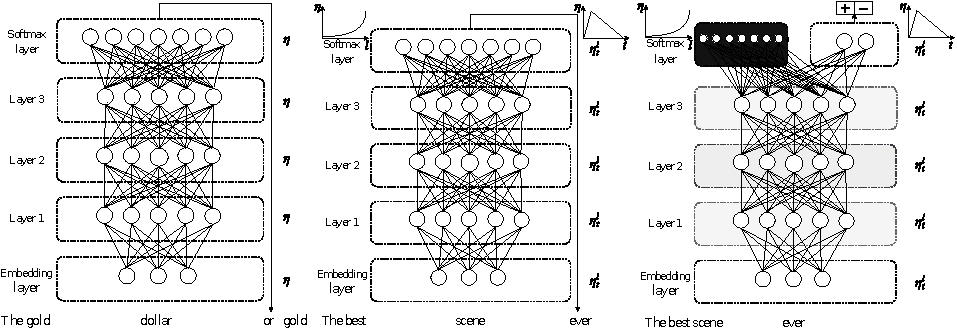
\includegraphics[width=\textwidth]{img/02/ulmfit.pdf}
    \caption{Universal Language Modeling for Text Classification (ULMFiT). Esquema del método planteado: primero se pre-entrena sobre la tarea de modelado de lenguaje sobre un dataset no supervisado. Luego, se corre la misma tarea pero sobre el texto de la tarea ignorando las etiquetas (ajuste de dominio). Finalmente, se agrega una capa de parámetros particulares de la tarea y se entrena la red completa descongelando gradualmente cada capa. Fuente: \citet{howard-ruder-2018-universal}}
    \label{fig:ulmfit}
\end{figure}

Alrededor de 2018, este paradigma de entrenar una red desde cero compartiendo su capa más baja --word2vec o bien \elmo{}-- comenzó a cambiar hacia un esquema donde se entrena una red neuronal sobre una tarea genérica para luego ajustarla a la tarea específica, una práctica muy común en el área de Visión por Computadora. \citet{howard-ruder-2018-universal} introdujeron la técnica de ULMFiT(Universal Language Modeling for Fine-tuning for text classification), uno de los trabajos fundamentales de este nuevo enfoque en NLP. ULMFiT consta de pre-entrenar en primer lugar un modelo de lenguaje sobre un gran dataset no etiquetado, y luego utilizar esa misma red (cambiándole la última capa) para ajustarla a una tarea específica. El primer paso, el \tbf{pre-entrenamiento} es realizado una única vez, y sus pesos son luego re-utilizados para realizar el ajuste en cada tarea distinta. Este es uno de los primeros esquemas de \tbf{transfer learning} exitosos sobre NLP: transferimos conocimiento de la tarea de modelado de lenguaje a las distintas tareas finales que realizamos como POS tagging, análisis de sentimientos, detección de entidades nombradas, etc.

Los autores proponen tres etapas: primero, el pre-entrenamiento sobre la tarea de modelado de lenguaje en un gran dataset de texto (e.g. Wikipedia o Common Crawl); segundo, un ajuste de la tarea de modelado de lenguaje sobre el texto de la tarea en cuestión (LM fine-tuning); y finalmente, el entrenamiento sobre las etiquetas de la tarea (Classifier fine-tuning). La figura \ref{fig:ulmfit} ilustra las tres etapas para el problema de clasificación de sentimientos. Entre varias técnicas que utilizan para entrenar estos modelos, vale destacar el uso de \emph{slanted triangular learning rates}, donde el learning rate tiene una etapa de \emph{warmup} donde sube hasta el pico y luego una etapa de \emph{annealing} donde se reduce linealmente hasta 0 por el resto del entrenamiento. Esta técnica es también utilizada por \bert{} y otros modelos de lenguaje basados en transformers.

El modelo de lenguaje utilizado por los autores de \emph{ULMFiT} utiliza una arquitectura \emph{AWD-LSTM} \cite{merity2018regularizing}. Estas arquitecturas recurrentes fueron el estado del arte para las tareas de modelado de lenguaje (y consecuentemente, para esquemas de transfer learning como el mencionado) pero fueron sobrepasados a los pocos meses por los modelos de lenguaje basados en \emph{transformers}.


\subsection{Traducción automática y atención}
\label{sec:02_transformers}


Hacemos a continuación una pequeña digresión sobre traducción automática y atención, conceptos necesarios antes de hablar de Transformers. El modelo \emph{encoder-decoder} permitió la utilización de redes neuronales para tareas de traducción de secuencias, es decir, donde queremos convertir $x = x_1 \ldots x_n$ a $y = y_1 \ldots y_m$, dos secuencias de diferente longitud. \citet{sutskever2014sequence} propusieron el siguiente esquema para abordar esta clase de tareas: en primer lugar, un \emph{codificador} (encoder) consume la cadena de entrada $x$,  conviertiéndola a un vector contextualizado $h$ de dimensión fija; y luego, un \emph{decodificador} (decoder) consume el vector de contexto $h$ para convertirlo a la cadena de salida $y$. Esto puede resumirse en las ecuaciones:

\begin{align*}
    h   &= \text{encoder}(x) \\
    y   &= \text{decoder}(h)
\end{align*}

Particularmente, los autores plantea un modelo basado en redes recurrentes (LSTMs) tanto para el \emph{encoder} como para el \emph{decoder}. El \emph{encoder} consume paso a paso la entrada, y el \emph{decoder} es esencialmente un modelo de lenguaje recurrente condicionado por el vector de entrada $h$.

Una de las limitaciones de las redes recurrentes es que sufren sesgo de \tbf{localidad} o \tbf{secuencialidad} (locality bias) \cite{battaglia2018relational}. En palabras coloquiales, las redes recurrentes tienen problemas para aprender dependencias de largo rango en las oraciones, siendo esto producto de su arquitectura autorregresiva donde se construye la salida $y_t$ en base a $y_{t-1}$. Este sesgo es particularmente dañino en tareas de tranducción de sequencias con la arquitectura encoder-decoder básica ya que a esto se le suma un cuello de botella forzoso por la compresión de toda la secuencia de entrada en el vector de dimensión fija $h$. Un síntoma de esto es observado en \citet{sutskever2014sequence}: invirtiendo la oración de entrada obtiene mejores resultados para la tarea de traducción automática.


\begin{figure}[t]
    \centering
    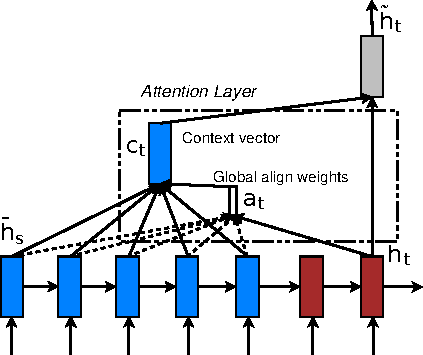
\includegraphics[width=0.5\textwidth]{img/02/attention_model.pdf}
    \caption{Mecanismo general de atención. En azul, la salida del encoder recurrente de la entrada. En rojo, la salida del decoder recurrente. Fuente: \citet{luong2015effective}}
    \label{fig:attention_mechanism}
\end{figure}


Los mecanismos de \emph{atención} \cite{bahdanau2014neural} ayudan a mitigar estas dificultades. A grandes rasgos, esta técnica agrega información adicional en cada paso del decoder mediante una combinación lineal de los estados ocultos del encoder. Recordemos que en la arquitectura básica propuesta en \citet{sutskever2014sequence} eran descartados, sólo siendo utilizado el estado final $h$. Describimos a continuación las ecuaciones de atención, que nos servirán para entender el mecanismo utilizado en la siguiente sección sobre Transformers.

Suponiendo que queremos traducir una secuencia $(x_1, \ldots , x_n)$ a $(y_1, \ldots , y_m)$, y que tenemos los estados ocultos $(\overline{h_1}, \ldots , \overline{h_n})$ generados en el encoder para la entrada, y los estados ocultos $(h_1, \ldots , h_m)$ y para la salida, el mecanismo de atención \footnote{global, en \citet{luong2015effective} se menciona el mecanismo local que no consideramos} consta de calcular para cada paso $t$ de la etapa de decodificación un vector de contexto

\begin{equation*}
    c_t = \sum_{i=1}^n \alpha_i^{(t)} \overline{h_i}
\end{equation*}

\noindent donde $\alpha^{(t)}$ es el vector de alineamiento, calculado como

\newcommand{\score}[0]{\text{score}}

\begin{equation*}
    \alpha^{(t)} = \softmax(\score(\overline{h_1}, h_t), \score(\overline{h_2}, h_t) \ldots , \score(\overline{h_n}, h_t))
\end{equation*}

\noindent Cada $\score(\overline{h_i}, h_t)$ marca una similaridad no normalizada entre sus argumentos. Las alternativas planteadas en \citet{luong2015effective} son:

\begin{equation}
    score(\overline{h_i}, h_t) =  \begin{cases}
        \overline{h_i}^T h_t   & \text{dot} \\
        \overline{h_i}^T W h_t & \text{general} \\
        v^T\text{tanh}(W [\overline{h_i}^T; h_t]) & concat
     \end{cases}
\end{equation}

% copypasting random stuff from the Internetz
% https://tex.stackexchange.com/questions/66537/making-hats-and-other-accents-bold
%
% \newcommand{\thicktilde}[1]{\mathbf{\tilde{\text{$#1$}}}}

\noindent con $W$ y $v$ parámetros adicionales. En el caso de la atención producto interno podemos reescribir todas las ecuaciones como:

\begin{equation}
    C = \softmax(H \widehat{H}^T ) \widehat{H}
    \label{eq:attention_product}
\end{equation}

\noindent donde $\widehat{H}, H$ son los vectores que tienen $(\overline{h_1}, \ldots , \overline{h_n})$  y $(h_1, \ldots , h_m)$ como filas respectivamente, y $\softmax$ se calcula fila a fila.

Finalmente, el vector $\widetilde{h_t}$ es calculado como una transformación del estado oculto del decoder $h_t$ y el vector contextual $c_t$:


\begin{equation*}
    \widetilde{h_t} = \tanh(W_h [h_t; c_t])
\end{equation*}


El vector $\widetilde{h_t}$ contiene información de todos los estados ocultos del codificador, atenuando los problemas de localidad de las redes recurrentes. Esta técnica se convirtió en parte integral de las tareas de traducción automática, resumen automático, entre otras. La figura \ref{fig:attention_mechanism} ilustra esta arquitectura.

La técnica de auto-atención o intra-atención \cite{parikh-etal-2016-decomposable} (self-attention en inglés) consiste en aproximadamente la misma idea que la atención sólo que teniendo una única secuencia; podemos asumir ecuaciones similares con $\overline{h_i} = h_i$. La auto-atención genera representaciones de los distintos vectores de entrada observando la totalidad de la secuencia, a diferencia de las redes recurrentes que sólo construyen una representación en base al paso anterior. Esta capa es utilizada en arquitecturas para clasificación de texto encima de una capa recurrente para generar representaciones con dependencias sin distinción de la distancia entre los distintos tokens.

\section{Transformers}

\begin{figure}[t]
    \centering
    \begin{subfigure}[t]{0.55\textwidth}
        \centering
        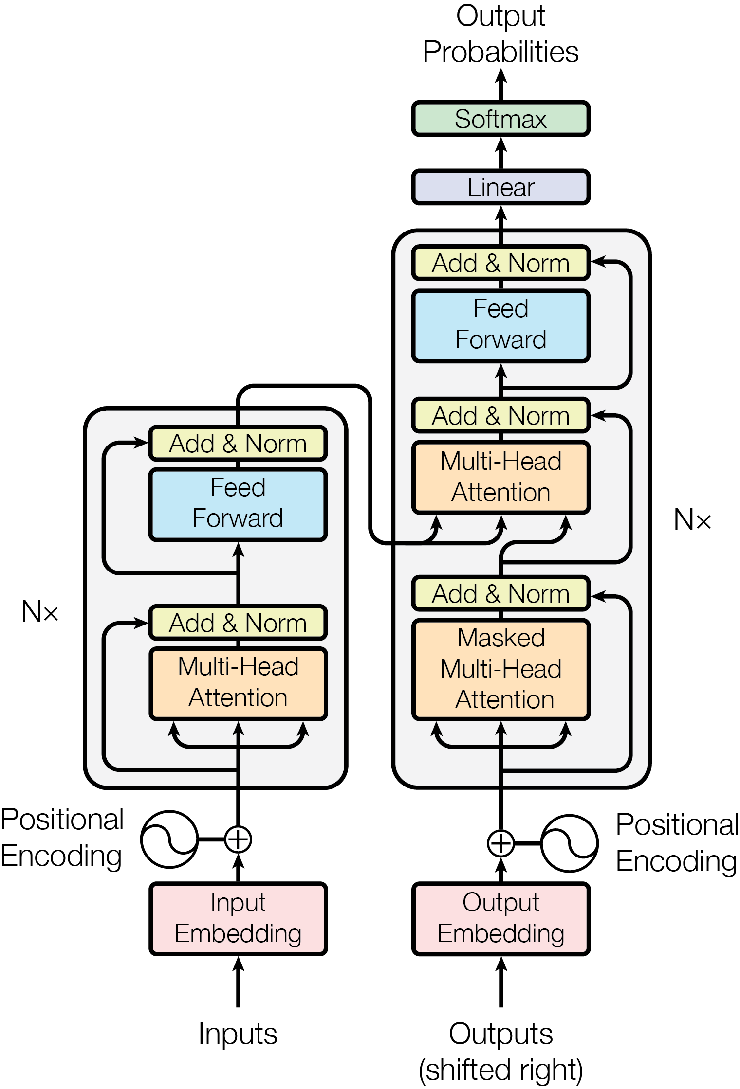
\includegraphics[width=0.55\textwidth]{img/02/transformer_architecture.png}
        \caption{Arquitectura de modelos Transformer}
        \label{fig:transformer_architecture}
    \end{subfigure}
    \begin{subfigure}[t]{0.40\textwidth}
        \centering
        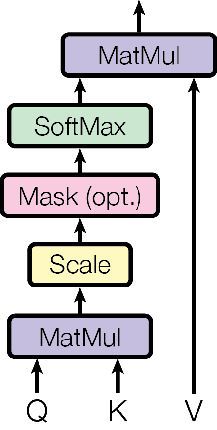
\includegraphics[width=0.40\textwidth]{img/02/scaled_self_attention.png}
        \caption{Mecanismo de scaled self-attention}
        \label{fig:scaled_self_attention}
    \end{subfigure}
    \caption{Modelo de transformador y su versión de auto-atención. La subfigura \ref{fig:transformer_architecture} muestra la arquitectura de los codificadores y decodificadores. Fuente: \citet{vaswani2017attention}}
    \label{fig:transformer_mechanism}
\end{figure}

Mencionamos el sesgo de la secuencialidad como uno de los problemas de las redes recurrentes. Otro de los grandes obstáculos para las arquitecturas autorregresivas es la paralelización. El cómputo secuencial donde $h_t$ se calcula en base a $h_{t-1}$ inhibe un cálculo paralelo, donde las diferentes representaciones puedan ser generadas simultáneamente. \citet{parikh-etal-2016-decomposable} es uno de los primeros trabajos que proponen una arquitectura para la tarea de inferencia (NLI) enteramente basada en una arquitectura de atención, sin ningún tipo de recurrencia.

\citet{vaswani2017attention} introdujeron la arquitectura \tbf{Transformer} para la tarea de traducción automática. Esta arquitectura no utiliza capas recurrentes ni convolucionales, basándose enteramente en el mecanismo de auto-atención. La figura \ref{fig:transformer_architecture} muestra la arquitectura de los modelos basados en Transformer, organizado en forma de encoder-decoder, con 6 capas de cada uno.

Cada capa del encoder utiliza un mecanismo de auto-atención múltiple seguido de una capa feed-forward punto a punto. Las dos capas de auto-atención o feed-forward están sucedidas por conexiones residuales \cite{he2016deep} para facilitar el flujo del gradiente en una arquitectura profunda y una capa de normalización, de manera que la salida se expresa como:

\begin{equation*}
    \text{Layer}(x) = \text{Norm}(x + \text{subLayer}(x))
\end{equation*}

Las capas decodificadoras son similares, salvo que se les agrega una capa extra de auto-atención donde se combinan las salidas del encoder con las representaciones que genera el decoder. A su vez, las capas de multi-atención están enmascaradas para no poder ``ver'' las representaciones que se generan en pasos posteriores para guardar su naturaleza secuencial en la tarea.

El cálculo de atención utilizado en este trabajo es similar al visto en la ecuación \ref{eq:attention_product}, aunque normalizado por $\sqrt{d_k}$, donde $d_k$ es la dimensión de los vectores de entrada:

\begin{equation*}
    Attention(Q, K, V) = \text{softmax}(\frac{Q^T K}{\sqrt{d_k}}) V
\end{equation*}

Cada capa utiliza varias cabezas de auto-atención, cuyas salidas son concatenadas y proyectadas. A su vez, la salida de cada una de las capa pasa por una regularización de tipo dropout \cite{srivastava2014dropout}.

Un punto a mencionar de los transformers es que, siendo que no tiene ningún tipo de recurrencia y convolución, carecen de cualquier ordenamiento de la secuencia de tokens. Para inyectar ese conocimiento en la red, utilizan \emph{vectores de posicionamiento} (positional embeddings) que se suman a los vectores de entrada de la capa de embeddings, como se ilustra en la figura \ref{fig:transformer_architecture}. Estos vectores no son parámetros entrenados (como sí lo son en \bert{}) sino que se calculan mediante funciones sinusoidales.


No nos extenderemos más en la explicación de esta arquitectura, y referimos para más información a los excelentes artículos \emph{Transformers from Scratch} \footnote{\url{http://peterbloem.nl/blog/transformers}}, \emph{Annotated Transformer} \footnote{\url{https://nlp.seas.harvard.edu/2018/04/03/attention.html}} y \emph{The Illustrated Transformer} \footnote{\url{https://jalammar.github.io/illustrated-transformer/}}.


\section{GPT, BERT y amigos}

\label{sec:02_bert}

Combinando las ideas de ULMFit --entrenamiento semi-supervisado sobre la tarea de modelado de lenguaje-- y la arquitectura Transformer --paralelización del cálculo mediante auto-atención -- en \citet{radford2018improving} se introduce GPT (\emph{generative pre-training}). Esta técnica consiste de un pre-entrenamiento sobre un gran corpus no etiquetado seguido de un fine-tuning discriminativo para cada tarea, muy en la línea de \citet{howard-ruder-2018-universal} introduciendo unos pocos parámetros específicos para cada una de estas. El modelo que usa esta tarea es el de \tbf{modelado de lenguaje causal} -- es decir, de izquierda a derecha. GPT obtuvo el estado de arte para el benchmark GLUE \cite{wang-etal-2018-glue}, superando a \elmo{} y otros.


\begin{figure}[t]
    \centering
    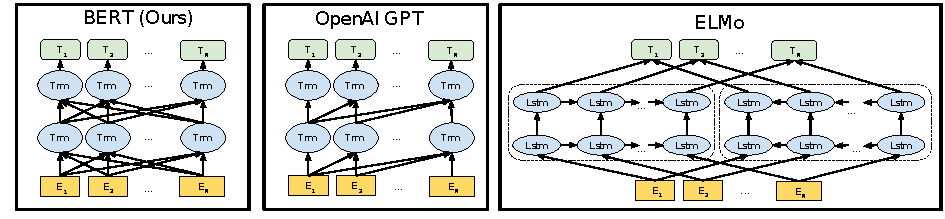
\includegraphics[width=\textwidth]{img/02/gpt_vs_bert.pdf}
    \caption{Comparación entre ELMo, GPT y BERT. ELMo genera vectores contextualizados mediante dos modelos de lenguaje recurrentes (uno de izquierda a derecha y el otro al revés), . GPT pre-entrena un modelo de lenguaje basado en Transformers. BERT genera representaciones bidireccionales }
    \label{fig:gpt_vs_bert_vs_elmo}
\end{figure}


\bert{} \cite{devlin2018bert} (Bidirectional Encoder Representations from Transformers) plantea una modificación sobre GPT: en lugar de pre-entrenar sobre la tarea de modelado de lenguaje \tbf{causal} --de izquierda a derecha-- hacerlo sobre la tarea de modelado de lenguaje \tbf{enmascarado}. Esta tarea (usualmente llamada \emph{Cloze task} \cite{taylor1953cloze}) consta de enmascarar una cierta cantidad de palabras de una frase, y luego intentar predecir las palabras faltantes. Por ejemplo, en la siguiente frase, consta de reemplazar los dos tokens \verb|[MASK]|:

\begin{center}
    El \verb|[MASK]| es celeste y el pasto \verb|[MASK]|
\end{center}


A diferencia de la tarea de modelado de lenguaje causal, los autores argumentan que esta tarea permite generar representaciones bidireccionales ricas. La figura \ref{fig:gpt_vs_bert_vs_elmo} muestra una comparación entre los distintos tipos de pre-entrenamiento de GPT.

BERT es pre-entrenado conjuntamente sobre dos tareas: una, la ya mencionada tarea de modelado de lenguaje enmascarado; la otra, la tarea de \emph{predicción de próxima oración} (Next Sentence Prediction, NSP). Esta tarea consiste en predecir si, dado un par de oraciones, la segunda es la que sigue a la primera. El 50\% de las ocasiones, las dos oraciones de entrada son contiguas en el texto de origen, y el 50\% restante son dos oraciones aleatorias concatenadas. Esta tarea debiera guardar cierta relación con la semántica de las oraciones y su interrelación, necesaria en tareas como NLI y Question Answering.

\newcommand{\clstok}[0]{\texttt{[CLS]}}
\newcommand{\septok}[0]{\texttt{[SEP]}}

\begin{figure}[t]
    \centering
    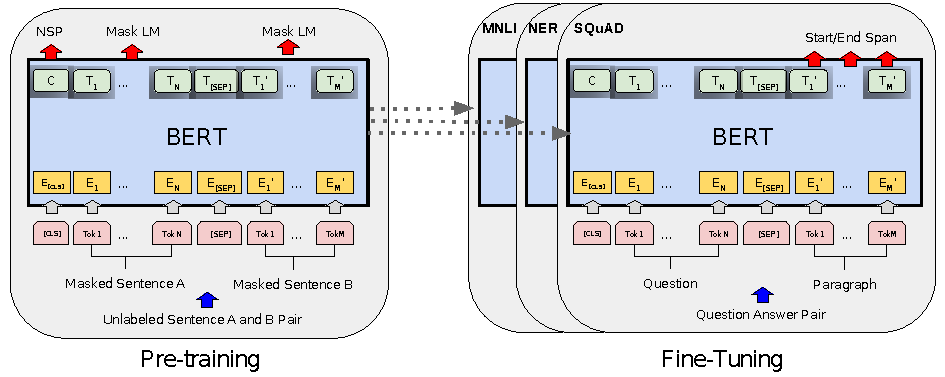
\includegraphics[width=\textwidth]{img/02/bert.pdf}
    \caption{Pre-entrenamiento y fine-tuning de BERT para distintas tareas. Fuente: \citet{devlin2018bert}}
    \label{fig:bert_pretraining_and_finetuning}
\end{figure}

Dos caracteres especiales son utilizados en \bert{}: \clstok{} y \septok{}. Estos caracteres se utilizan para delimitar las oraciones en la entrada de la red, y también para separar las dos oraciones de entrada. Durante el pre-entrenamiento, la representación generada por \clstok{} es utilizada como la predicción de la tarea NSP y la representación de cada token enmascarado es utilizado como entrada de una capa softmax para predecir el token faltante. Para la mayoría de las tareas de clasificación de texto, \clstok{} es usado como la representación de la (o las) oraciones de entrada. La figura \ref{fig:bert_pretraining_and_finetuning} ilustra esta metodología para la tarea de QA, ligeramente más compleja que la clasificación de texto.

\bert{} utiliza WordPiece \cite{wu2016google}, un algoritmo de tokenización muy similar a BPE \cite{sennrich2016neural}, con un vocabulario de largo 30,000 para separar su entrada en subpalabras de manera eficiente. A su vez, para cada posición de su entrada entrena embeddings posicionales (a diferencia de los embeddings posicionales fijos originales de \citet{vaswani2017attention}) con un límite de 512, y dos embeddings especiales para la primer oración y la segunda oración de la entrada. Los vectores que ingresan a la primer capa de transformers son la suma de los embeddings de cada token, los embeddings posicionales, y los embeddings de oración.

El proceso de pre-entrenamiento es realizado sobre la concatenación de dos corpus: BooksCorpus \cite{zhu2015bookscorpus} y la versión en inglés de Wikipedia. Estas dos fuentes son utilizadas ya que permiten extraer pares de palabras contiguas, algo necesario para la tarea de NSP.


\citet{liu2019roberta} proponen dos modificaciones al pre-entrenamiento de \bert{}: en primer lugar, remover la tarea de NSP; y en segundo lugar, realizar un pre-entrenamiento más extenso y con batch sizes más grandes, pasando de lotes de 512 a 8,192 oraciones. Este modelo pre-entrenado (al cual se denomina \roberta{}) obtuvo mejor desempeño que \bert{} en el dataset de GLUE y otras tareas.

Luego de estos modelos de lenguaje, una suerte de guerra armamentística tuvo lugar para entrenar arquitecturas más grandes y con más parámetros al observar que aumentando la cantidad de estos mejoraba la performance en distintas tareas -- sin observarse aún un techo más que los recursos computacionales y energéticos disponibles en el planeta. Sólo para ilustrar el punto, la versión \emph{base} de \bert{} tiene 110M parámetros, su versión large 330M, GPT-2 1,500M, Turing NLG de Microsoft 17,000M y finalmente GPT-3 \cite{brown2020language} tiene la asombrosa cantidad de 175,000 M parámetros.
\part{Trabajos con datasets existentes}

\chapter{Análisis de Sentimientos}
\label{chap:03_social_text_classification}

La extracción de opiniones en distintos espacios virtuales ha atraído mucho interés desde los comienzos de la Web 2.0. Inicialmente motivados por fines puramente comerciales, diferentes oportunidades han surgido mediante al desarrollo de la técnica y la mayor interacción de usuarios en Internet: desde fines sociológicos --como el análisis de discurso de odio o las reacciones a la pandemia-- hasta políticos -- como observar cuál es la opinión general sobre tal o cual candidato o sobre un tema candente. A partir de los años 2000, y debido a la combinación del desarrollo de métodos de aprendizaje estadístico y la cantidad creciente de datos disponibles generados por usuarios en Internet, numerosos trabajos han analizado este tipo de textos para poder extraer conocimiento \textbf{subjetivo} de quienes vuelcan sus pensamientos en las redes sociales y otros espacios virtuales.

Debido a la inmensa cantidad de contenido generado en diversos sitios y redes sociales (se estima que en el mundo se generan 500 millones tweets por día para 2021\footnote{Fuente: \url{https://www.internetlivestats.com/twitter-statistics/}}), esta tarea es difícil de realizar sin algún tipo de automatización. Para ello, muchísimo esfuerzo se ha volcado en utilizar técnicas de aprendizaje automático para poder extraer este tipo de información de los textos creados por usuarios. El avance de las técnicas de NLP --como hemos descrito en el capítulo anterior-- han permitido avanzar sobre este terreno; sin embargo, muchas de las limitaciones actuales del área junto a las dificultades particulares de las interacciones en medios sociales hacen esta tarea difícil.

En este capítulo haremos una breve introducción al análisis de sentimientos o extracción de opiniones sobre textos de redes sociales. Esto es, dado un texto generado por un usuario (un post en Facebook, Instagram, un tweet, etc) predecir alguna característica discreta de éste, como por ejemplo si es un texto positivo o negativo, si tiene algún tipo de emoción de ira, alegría, u otra; si contiene discurso de odio contra algún grupo o no; si es irónico; entre otras. En base a datasets en español para distintas tareas, presentaremos modelos de clasificación basados en técnicas del estado del arte.

Analizaremos también algunas cuestiones relacionadas a la adaptación de dominio y representaciones generadas sobre dominios de textos generados por usuarios, planteando algunas líneas que retomaremos en capítulos posteriores.


\section{Motivación}

Las motivaciones para extraer opiniones subjetivas de usuarios en Internet son múltiples, aunque intentaremos categorizarlas en algunos grupos de notable interés. Dado el aumento considerable de contenido generado por usuarios desde la popularización de la WWW  --y subsiguientemente con la explosión de las Redes Sociales-- una de las cuestiones que motoriza este área es netamente comercial: ¿qué opinan los usuarios sobre este nuevo producto? ¿cuáles creen que son sus falencias? ¿qué tal es el servicio en tal o cual Restaurant? Desde ya más de 20 años, numerosos sitios y aplicaciones brindan la posibilidad de que los clientes vuelquen sus opiniones al respecto de los productos que consumen en sus plataformas. Para citar unos ejemplos, IMDb permite agregar comentarios sobre películas, Google Maps sobre distintos sitios --tanto turísticos como locales comerciales--, o los distintos sitios de venta minorista como MercadoLibre, eBay, o Amazon sobre los productos que compran sus usuarios. Sobre esta información disponible, una encuesta de 2008 \cite{horrigan2008online} reportó que cerca del 81\% de los usuarios de Internet de entonces (60\% de los habitantes de Estados Unidos) realizaron investigación online antes de sus compras, aunque también reportaban problemas a la hora de encontrar información valiosa para sus fines.

Con la explosión de las redes sociales, nuevas oportunidades y posibilidades de preguntas a contestar se abrieron mediante la extracción de opiniones en este medio \footnote{Si bien algunas preguntas de carácter sociológico tuvieron lugar con anterioridad, podemos marcar el uso intensivo de Facebook y Twitter como el comienzo de un estudio más sistemático de ellas dado el enorme volumen de datos accesibles para los investigadores}. Uno de estos horizontes, que es de interés particular para esta tesis, es el de las preguntas de carácter sociológico y político. Preguntas que pueden suscitar interés dentro de este punto pueden ser:

\begin{itemize}
    \item ¿cuál es la opinión de los usuarios acerca de la legalización del aborto en cierto país que tiene en tratamiento este tema? ¿es representativo de la población en general? \cite{graells2019abortion}
    %\item ¿cuál es el sentimiento que tienen ciertos usuarios hacia los inmigrantes subsaharianos en España?
    \item ¿cómo se ha modificado el humor social de acuerdo a crisis económicas o pandemias como la del COVID-19? \cite{brufau2020emotion}
    \item ¿qué características tiene el discurso de odio  contra los inmigrantes en España en el medio del auge de la ultraderecha en dicho país? \cite{calderon2020topic}
    \item ¿qué artículos periodísticos suscitan la mayor cantidad de discurso discriminatorio en las redes sociales?
    \item ¿cuáles son las principales vulnerabilidades e intereses de ciertos sectores de la población? \cite{zuiderveen2018online} \footnote{Esto, según parece, fue utilizado en el affaire de Cambridge Analytica en las elecciones de 2016 que consagraron a Donald Trump en EEUU}
\end{itemize}

entre otras. Estos tópicos son de gran interés para investigadores y políticos. Usualmente, la forma más estandarizada de acceder a la opinión de distintos actores sociales ha sido la de encuestas; sin embargo, la recolección y extracción automática de opiniones de medios virtuales brinda una alternativa (a veces) más económica y masiva aunque con un sesgo poblacional distinto al de otras metodologías.

\section{Clasificación de textos sociales}

Muchos de estos problemas de extracción de opiniones se pueden plantear como tareas de clasificación de texto \cite{pang2008opinion}. El análisis de polaridad se puede plantear como una tarea de predecir si un texto tiene un sentimiento positivo, negativo, o neutro. El análisis de emociones se puede plantear (entre otras formas) como la de predecir la emoción predominante en el texto sobre un conjunto de seis posibles emociones.

Algunas variantes de estos problemas se pueden dar en el contenido analizado. El \emph{Análisis de Sentimiento basado en aspectos} (usualmente denominada \emph{ABSA} en la literatura por sus siglas en inglés) es una variante de la clasificación de polaridad en la que queremos predecir el sentimiento de un texto para cierto aspecto \cite{pavlopoulos2014aspect}; por ejemplo, en la oración ``lindo lugar, la comida está muy bien pero la cerveza es horrible'' (en una posible reseña de un restaurant) podemos identificar dos sentimientos distintos: uno positivo para la comida y otro negativo para la cerveza. Dentro de estos problemas que complejizan la entrada, podemos contar algunos de carácter multimodal: en \citet{sharma-etal-2020-semeval} se plantea un problema de análisis de emociones para memes donde la entrada (el contenido social) consta de imágenes y texto, y se intenta predecir la emoción predominante.

Análogamente, se puede agregar cierta complejidad en la salida. El \emph{Stanford Sentiment Treebank (SST)} \cite{socher-etal-2013-recursive} plantea una tarea de análisis de polaridad asignando una escala de Likert \cite{likert1932technique} donde cada comentario está etiquetado como muy negativo, algo negativo, neutral, algo positivo o muy positivo. Así mismo, otra posibilidad es la de predecir conjuntamente varias variables: por ejemplo, predecir si un comentario es discriminatorio, si es dirigido a un grupo o una persona, y si es agresivo, como el dataset de hatEval \cite{hateval2019semeval}; o bien, dado un comentario de una nota periodística, predecir las características que discrimina si es que hay alguna (como ser a las mujeres, al colectivo LGBTI, por motivos raciales, etc). De este último ejemplo hablaremos en los capítulos \ref{chap:05_dataset_creation} y \ref{chap:06_contextualized_hate_speech}.


\section{Trabajo previo}

El análisis de sentimientos, opinion mining u opinion extraction suscitó interés casi desde el comienzo de la generación masiva de contenido de parte de los usuarios en la WWW. Particularmente desde la eclosión de las redes sociales, la inmensa cantidad de contenido generado por usuarios ha sido una fuente de información sin antecedentes para la extracción de todo tipo de opiniones. La bibliografía que comprende este tema es demasiado extensa y escapa los objetivos de esta tesis centrada en la detección de discurso de odio. Mencionamos algunos surveys relevantes y una pequeña selección de trabajos a continuación.

\citet{pang2008opinion} ofrecen un amplio repaso sobre los usos, aplicaciones, técnicas y dificultades de la extracción de opiniones en la era pre-deep learning y pre-redes sociales, mencionando cuestiones como las dificultades que los diferentes dominios presentan a las técnicas del entonces estado del arte. El trabajo de \citet{pak2010twitter} es uno de los pioneros en plantear a Twitter como una fuente de mensajes para la extracción de opiniones -- en particular, para analizar polaridad de mensajes -- proponiendo una metodología para recolectar y etiquetar datasets sobre esta red social. \citet{yue2019survey} presentan un racconto de los diversas tareas de análisis de sentimientos aplicados a textos de redes sociales y las técnicas para atacarlo.

Dentro de los recursos para tareas de opinion mining, \citet{maas-EtAl:2011:ACL-HLT2011} presenta un dataset de análisis de polaridad con dos etiquetas (positivo y negativo) sobre películas en la plataforma de IMDb, extensamente utilizado para la tarea de análisis de sentimientos. El Stanford Sentiment Treebank (SST) \cite{socher-etal-2013-recursive} es un dataset que contiene información granular en una escala símil Likert de polaridad sobre las distintas subpartes de cada oración. Esta tarea forma parte del benchmark de General Language Understanding Evaluation (GLUE) \cite{wang-etal-2018-glue}. El workshop SemEval \footnote{\url{https://semeval.github.io/}} ha generado numerosos recursos para tareas de opinion mining en redes sociales, como Análisis de Polaridad, Análisis de Polaridad basado en aspectos, análisis de emociones, entre otras.

Centrándonos en los recursos y tareas en español, uno de los principales polos de esto es el Taller de Análisis de Sentimientos (TASS) \cite{overview_tass2018,garcia2020overview,cumbreras2016overview} organizado por la Sociedad Española de Procesamiento Natural (SEPLN) y a partir de 2020 en el marco del evento Iberian Languages Evaluation Forum (IberLEF). En este foro se presentaron tareas y datasets de análisis de sentimiento \cite{garcia2020overview}, de emociones\cite{plaza-del-arco-etal-2020-emoevent}, de toxicidad \cite{taule2021detoxis}, entre otras.


\section{Tareas analizadas}
\large
\begin{table}[t]
    \centering
    \begin{tabular}{| l | ll ll|}
        \hline
        Tarea                     &  Dataset                   & Tamaño         & Clases   &\\
        \hline
        \mr{3}{Análisis de Sentimientos}  &  \mr{3}{TASS 2020} & \mr{3}{14,509} & Neg      & (39.80\%)\\
                                          &                    &                & Neu      & (29.52\%)\\
                                          &                    &                & Pos      & (30.68\%)\\
        \hline
        \mr{7}{Análisis de emociones}&\mr{7}{TASS 2020/EmoEvent}&\mr{7}{8,409}  & Otra     & (49.08\%)  \\
                                          &                    &                & Alegría  & (21.58\%)  \\
                                          &                    &                & Tristeza & (12.00\%)  \\
                                          &                    &                & Ira      & (10.19\%)  \\
                                          &                    &                & Sorpresa & (4.10\%)  \\
                                          &                    &                & Disgusto & (1.91\%)  \\
                                          &                    &                & Miedo    & (1.14\%)  \\
        \hline
        \mr{2}{Detección de ironía}  & \mr{2}{IroSVa 2019}     & \mr{2}{9,000}  & No irónico   & (66.68\%)\\
                                          &                    &                & Irónico      & (33.32\%)\\
        %Análisis de Emociones     &  TASS 2020/EmoEvent\cite{plaza-del-arco-etal-2020-emoevent} & 7 & 1,879 \\
        \hline
    \end{tabular}
    \caption{Tareas evaluadas en este capítulo, junto a datos estadísticos de los datasets utilizados}
    \label{tab:03_tasks}
\end{table}

Analizamos 3 tareas de extracción de opiniones sobre redes sociales y las usamos como benchmark para las diferentes técnicas de clasificación. La tabla \ref{tab:03_tasks} contiene información sobre las distintas tareas analizadas y los datasets utilizados para ellas. Una de las tareas analizadas es la de \textbf{análisis de polaridad}: dado un tweet, detectar si tiene una polaridad general positiva, negativa, o neutra. Utilizamos el dataset de TASS 2020 \cite{garcia2020overview}, anotado con estas 3 clases y con información de las diferentes variedades dialectales del español a la que pertenece cada tweet. Para nuestro análisis, ignoramos estas distinciones y fusionamos todos los datos en un solo conjunto de datos (con las 3 particiones correspondientes de entrenamiento, validación, y test).


Para el análisis de emociones, también usamos el conjunto de datos de TASS 2020 \emph{EmoEvent} \cite{plaza-del-arco-etal-2020-emoevent}. Este dataset multilingual (español e inglés) contiene tweets etiquetados con las seis emociones básicas de Ekman \cite{ekman1992argument} :\emph {ira}, \emph {disgusto}, \emph {miedo}, \emph {alegría}, \emph {tristeza}, \emph {sorpresa} y también una emoción \emph{neutral}. El dataset fue recolectado en base a a ocho eventos globales diferentes de diferentes dominios (políticos, entretenimiento, catástrofes o incidentes, conmemoraciones globales, etc.) por lo que las emociones siempre están relacionadas con un fenómeno en particular. Solo conservamos la parte en español, que contiene 8.409 tweets.


 La \textbf{detección de ironía} también es una tarea que ha ganado popularidad recientemente. Algunos trabajos han mostrado que tiene importantes implicaciones en otras tareas de NLP de caracter semántico, como por ejemplo \citet{gupta-yang-2017-crystalnest} muestran que el uso de funciones derivadas de la detección de sarcasmo mejora el rendimiento en la tarea de análisis de sentimientos. Además de esto, el contenido generado por los usuarios es una rica y vasta fuente de ironía, por lo que esta tarea es de particular importancia para el dominio de las redes sociales. IroSVa \cite {ortega2019overview} es un dataset en Español (publicado en el contexto de TASS 2019) que tiene la particularidad de considerar los mensajes no como textos aislados sino con un contexto dado (un titular o un tema). Consta de 7.200 instancias y 1.800 ejemplos de prueba divididos en tres variantes geográficas de Cuba, España y México, cada una con una etiqueta binaria que indica si el comentario contiene ironía o no. A diferencia de las tres tareas anteriores mencionadas aquí, este conjunto de datos contiene no solo mensajes de Twitter, sino también de comentarios de noticias y foros de debate como 4forums.com y Reddit.

 La tabla \ref{tab:03_datasets_examples} ilustra algunos ejemplos seleccionados para las distintas tareas y sus clases. En el caso de la tarea de detección de emociones, podemos ver que algunos ejemplos han sido preprocesados por sus autores para ocultar los hashtags y urls.

\begin{table}
    \centering
    \begin{tabularx}{\textwidth}{l l X}
        Tarea                          & Clase        &            \\
        \hline
        \mr{7}{Emociones}              & Neutral        & Espectantes para ver el tercer capitulo de HASHTAG. El principio empieza bien.	\\
                                       & Alegría        & Lo de Messi ha sido increíble! HASHTAG        \\
                                       & Tristeza       & Un día lamentable. Se perdieron años de historia, de cultura, de arquitectura... Me siento devastada al ver las imágenes del incendio de la catedral de HASHTAG en HASHTAG URL \\
                                       & Ira            & URL que discurso para ponerlo a llorar, Putos humanos, para cuando la extinción?? \\
                                       & Sorpresa       & Santa Maria Madre de Dios HASHTAG URL \\
                                       & Miedo          & Joder, izquierda venció ¿y qué? A mi me preocupa y mucho que Vox haya pasado de 0 a 24!! ¿a nadie le parece un montón? No sé, debo ser idiota. HASHTAG	\\
                                       & Disgusto       & Como se nota que HASHTAG ya no tiene el apoyo de los libros. Vaya mierda de temporada se están sacando.	 \\
        \hline
        \hline
        \mr{3}{Sentimientos}           & Negativo       & que triste es la realidad	\\
                                       & Positivo       & Hola a todos corazones, buen día Y FELIZ NAVIDAD A TODOS USTEDES! DIOS ME LOS BENDIGA Y ME LOS LLENE DE TODO SU AMOR \\
                                       & Neutral        & $@$AlfonsoEmilioL La próxima vez que no vea lo entrevisto y pregunto que escucha.	\\
        \hline
        \hline
        \mr{4}{Ironía}                 &\mr{3}{Irónico} & Pues, noticia de última hora, eres un anormal que no sabe escribir. Es LESIONARAN.    \\
                                       &                & El juez paraliza la exhumación de Franco alegando peligro para los operarios. Pues me parece muy bien, porque con las ratas hay que ser muy precavido.	\\
                                       &                & $@$CristinaSegui\_ $@$Pablo\_Iglesias\_ Doctorado en cambiar pañales.....	\\
                                       & No irónico     & No me sirvió para nada todo fue en vano. Espero mejore la calidad.	\\
        \hline
    \end{tabularx}
    \caption{Tareas evaluadas en este capítulo, junto a datos estadísticos de los datasets utilizados}
    \label{tab:03_datasets_examples}
\end{table}



\section{Normalización y preprocesamiento}
\label{sec:03_preprocessing}

Una de los pasos más importantes para la manipulación de texto social es el preprocesamiento. Con esto nos referimos al conjunto de técnicas dedicadas a disminuir la variabilidad del texto y aproximarlo a una forma lo más normal posible \footnote{\citet{eisenstein2013bad} discute siquiera que exista tal forma normal}. El texto generado por usuarios en medios informales suele ser más irregular que el texto proveniente de otras fuentes, con errores ortográficos y usos coloquiales que hacen difícil el tratamiento por algoritmos de NLP. Para poner un ejemplo, la frase ``¡qué lindo día, loco!'' puede ser representada de las siguientes maneras:

\begin{itemize}
    \item q lindo día loco
    \item k lindo diaaaaaaaa loco
    \item ke lendo diaa lk
\end{itemize}

\noindent entre otras formas posibles. Uno de los primeros trabajos que aborda este problema para el dominio de redes sociales es el de \citet{han2011lexical}. En base a un dataset de tweets, observaron que las palabras fuera de vocabulario (OOV en inglés) \footnote{fuera del vocabulario de un diccionario estándar de GNU en inglés} en dicha red social tienen una alta frecuencia de incidencia. Ejemplos de estas palabras son neologismos, errores ortográficos, typos, contracciones típicas de esta red social (lk), sustituciones fonéticas (wacho en vez de guacho), entre otras. Este problema de la desnormalización del texto generado por usuarios planteaba un serio inconveniente para los métodos del estado del arte de ese entonces basados en bolsas de palabras o representaciones sobre palabras aisladas \footnote{Recordemos que para el momento de la publicación de este trabajo aún no se usaban redes neuronales, word embeddings, ni mucho menos métodos más avanzados como \emph{fasttext}, que ayuda mucho en las palabras OOV}. Para mitigar la alta dimensionalidad que generan estas palabras fuera de vocabulario, los autores proponen diversas estrategias para normalizar las palabras y testean sus métodos sobre datasets de Twitter y SMS.

\citet{eisenstein2013bad} trata desde una perspectiva más amplia los enfoques utilizados hasta el momento. El autor plantea dos posibilidades para las tareas de NLP en el medio social: la \textbf{normalización} sería una forma de adaptar el texto a las herramientas, mientras que la \textbf{adaptación de dominio} sería adaptar las herramientas al texto. Con lo primero nos referimos al conjunto de técnicas que podemos utilizar para acercar la distribución del texto lo más posible a un dominio formal (por ejemplo, sobre el que entrenamos un POS tagger), mientras que por adaptación de dominio nos referimos a la construcción de datasets y algoritmos particulares para distintas tareas de NLP en redes sociales, como por ejemplo POS tagging \cite{gimpel2010part}, NER \cite{ritter2011named}, entre otros.

Con el advenimiento de las redes neuronales y los word-embeddings como GloVe o word2Vec, la alta desnormalización siguió siendo un escollo ya que cada representación se calcula sobre cada una de estas palabras. En el caso de una palabra fuera de vocabulario, un mecanismo habitual es asignarles un token especial ``<unk>'', y por lo tanto, una única representación para todas esas palabras OOV. Sin embargo, esto puede ser problemático ya que elimina muchas palabras similares a otras que sí tenemos en el vocabulario. \citet{bojanowski16} propuso una solución a esto al permitir formar la representación de cada palabra mediante una combinación lineal de las representaciones de las ``subpalabras'' de cada una (ver sección \ref{sec:02_representaciones}).

Con el advenimiento de los modelos basados en transformers, otros tipos de tokenización fueron propuestos que permiten reducir las palabras OOV. BPE \cite{sennrich2016neural}, Word Piece, Sentence Piece \cite{kudo-richardson-2018-sentencepiece} utilizan, en lugar de separar el texto mediante los espacios, en la utilización de distintos tipos de subpalabras. Esta técnica permite reducir la incidencia de palabras OOV notablemente.

En el caso de modelos basados en transformers entrenados sobre texto social, \citet{dat2020bertweet} plantearon experimentos en tareas sociales usando dos formas de normalización: una \textbf{débil}, donde sólo convierten nombres de usuario en un token especial \verb|@USER| y a las urls en otro token especial \verb|HTTPURL|, y otra estrategia \textbf{fuerte} donde usan diccionarios de normalización. Para un conjunto de tareas de clasificación sobre Twitter y distintos modelos pre-entrenados, los resultados de los experimentos arrojaron que la normalización fuerte empeora levemente la performance.

En base a esto, adoptamos una estrategia similar a la normalización \textbf{débil} mencionada en \citet{dat2020bertweet}:

\begin{itemize}
    \item Convertimos los handles a un token especial \verb|@usuario|
    \item Convertimos URLS a un token especial \verb|URL|
    \item Convertimos los emojis a representaciones textuales usando la librería \emph{emoji} \footnote{\url{https://pypi.org/project/emoji/}}
    \item Normalizamos risas (``jajajajjjjajaja'' lo convertimos a ``jaja'')
    \item Procesamos hashtags: \#EsteHayQueNormalizar lo convertimos a \emph{hashtag esto hay que normalizar}
    \item Limitamos repeticiones de caracteres a 3 ocurrencias
\end{itemize}

Si bien en algunas secciones (como en \ref{sec:04_preprocessing}) usaremos variaciones de estos métodos --particularmente para modelos lineales--, en general seguiremos esta estrategia de normalización.

\section{Modelos de clasificación}
\label{sec:03_classification}

\begin{figure}
    \centering
    % Link a draw
    % https://docs.google.com/drawings/d/1bSCMXkAF12gK4GFYL8tyIAPCMq4kj8JXovrf2lx5w_g/edit
    \begin{subfigure}[t]{\textwidth}
        \centering
        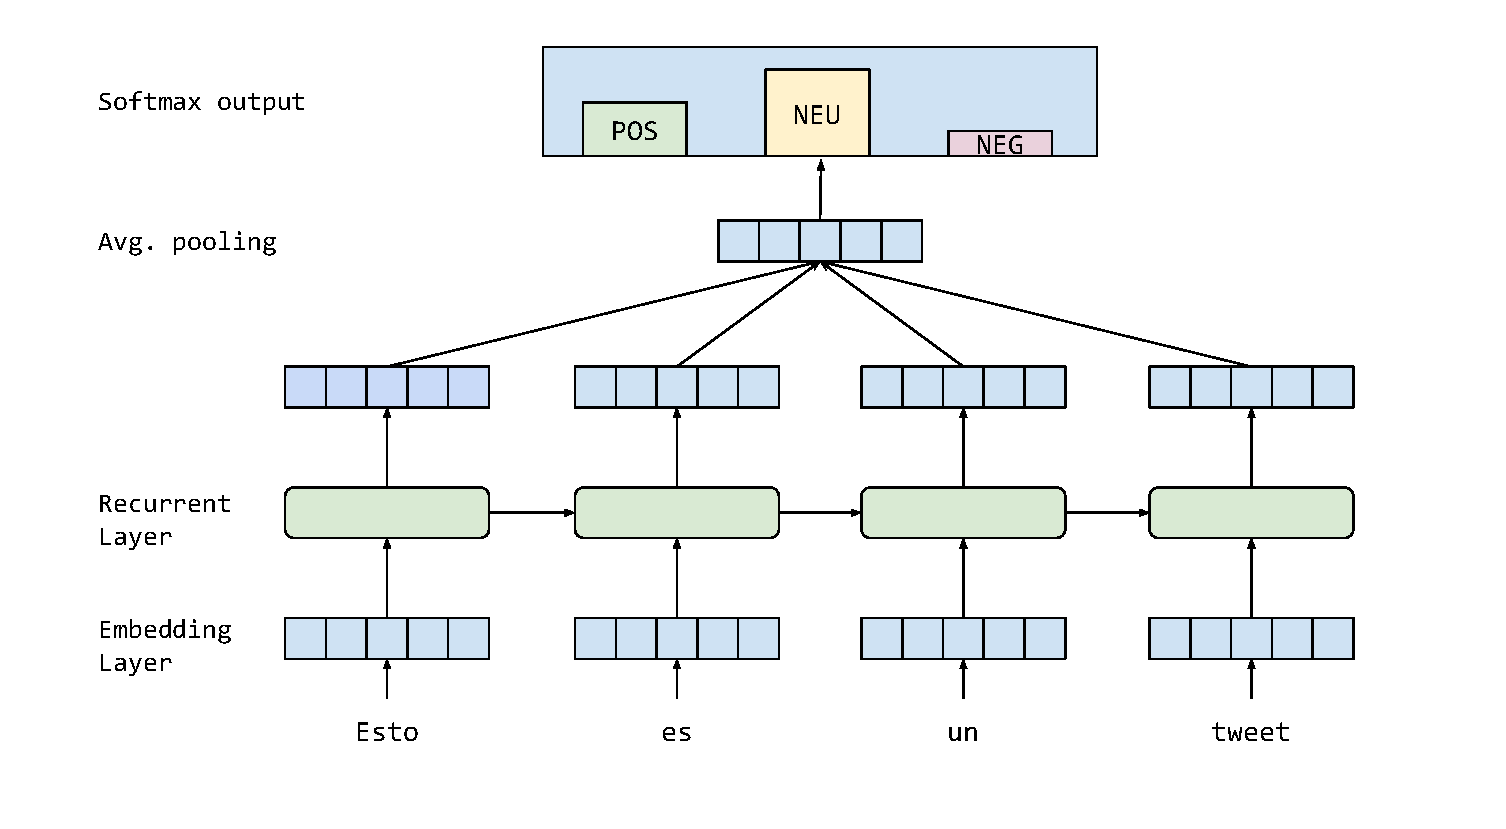
\includegraphics[width=\textwidth]{img/03/recurrent_classifier.pdf}
        \caption{Clasificador basado en redes recurrentes}
        \label{subfig:rnn_classifier}
    \end{subfigure}
    % Link a draw
    % https://docs.google.com/drawings/d/1KWz2NJGVoTO-pAAhhLjoX4AT-kSbK3yapLKLuQ2E9zw/edit
    \begin{subfigure}[t]{\textwidth}
        \centering
        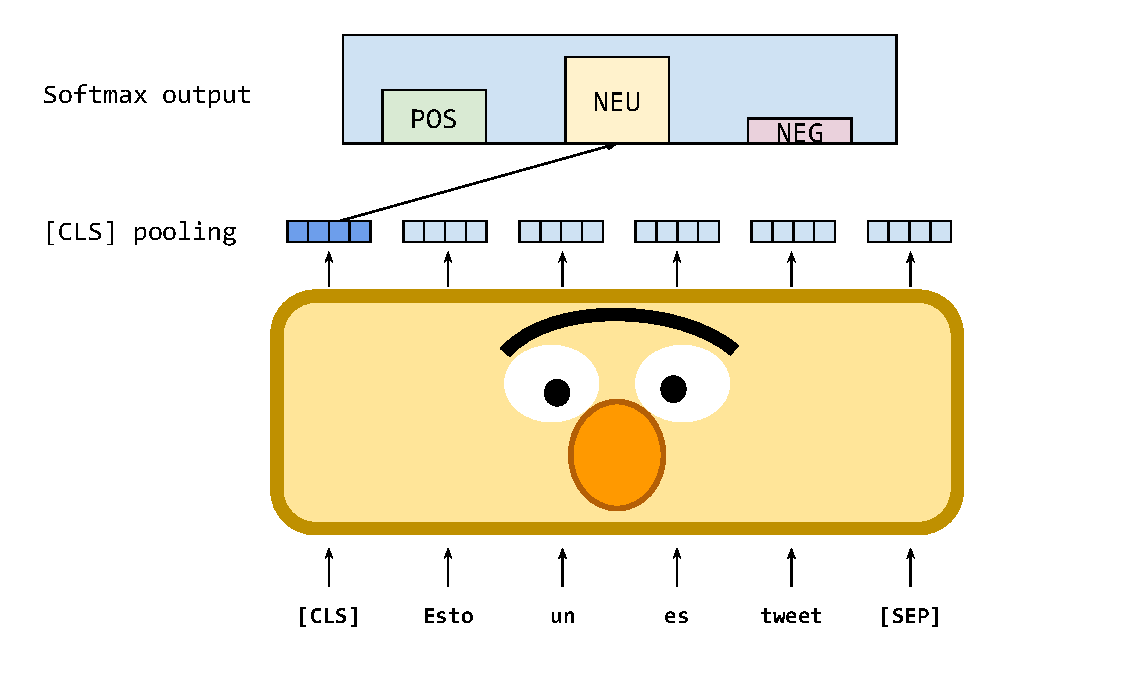
\includegraphics[width=\textwidth]{img/03/bert_classifier.pdf}
        \caption{Modelos de clasificación basado en BERT y símiles}
        \label{subfig:bert_classifier}
    \end{subfigure}

    \caption{Clasificadores propuestos para las tareas de Análisis de Polaridad, Análisis de Emociones y Detección de Ironía. La subfigura \ref{subfig:rnn_classifier} muestra la arquitectura del modelo recurrente, que usa una capa de embeddings basados en \emph{fasttext} y codifica el tweet como el promedio de las salidas de la capa recurrente. La subfigura \ref{subfig:bert_classifier} muestra un clasificador basado en BERT, donde tomamos la salida del token \clstok{} como la codificación del tweet. Ambos usan un decodificador softmax}
    \label{fig:03_classifiers}
\end{figure}

Describimos a continuación los clasificadores utilizados para las tareas. Podemos, a grandes rasgos, describir a todos nuestros clasificadores como compuestos de dos partes: un \emph{codificador} (o \emph{encoder} en inglés) que genera una representación contínua de longitud fija del texto de entrada, y un \emph{decodificador} que toma esa codificación y la convierte a la salida deseada.

Todas las tareas analizadas son de clasificación multiclase: elegir exactamente una clase entre varias. Para ello, nuestro decodificador será de la forma $\softmax(Wx + b)$, donde $W$ es una matriz de pesos y $b$ un vector de bias, ambos parámetros de nuestra red neuronal. Los modelos planteados diferirán entonces en los codificadores. Proponemos las siguientes variantes:

\begin{itemize}
    \item \textbf{FFN}: Un perceptrón multicapa (feed-forward network) con una función de activación intermedia \emph{ReLU}
    \item \textbf{GRU/biGRU}: Una red neuronal recurrente. La capa oculta es una Gated Recurrent Unit (GRU) unidireccional o bidireccional.
    \item \textbf{BETO|mBERT|RoBERTa|BERTin}: un modelo pre-entrenado de lenguaje basado en transformers.
\end{itemize}

En el caso de la \textbf{FFN}, la codificación se da luego de aplicar la función ReLU a la capa intermedia de la red. En el caso de la \textbf{GRU/biGRU}, la codificación se da como el promedio de los vectores salida de cada paso (podemos pensar cada uno de estos como representaciones contextualizadas de cada palabra). En el caso de los modelos basados en transformers, la codificación se da tomando la salida del caracter de inicio (\clstok{} en el caso de BERT pero puede variar para RoBERTa u otros modelos)\footnote{Si bien podría también tomarse el promedio como en el caso de las redes recurrentes, los modelos basados en transformers no sufren el cuello de botella que se genera tomando la última representación de la red recurrente}. La figura \ref{fig:03_classifiers} ilustra la arquitectura de los clasificadores recurrentes y basados en transformers.

Usamos un tamaño oculto de 512 para los modelos recurrentes y FFN, y para todos los casos un dropout \cite{srivastava2014dropout} de 0.1 sobre la codificación del tweet. Para los dos primeros modelos, los entrenamos usando Adam \cite{kingma2014adam} con un learning rate de 0.001 y un decay de 0.01. Para los modelos basados en transformers, usamos Adam con un learning rate triangular de $10^{-5}$ y un warmup del 10\% de los pasos. Entrenamos todos los modelos por 5 epochs y nos quedamos con los modelos que mejor performance tengan sobre el split de validación en términos de la métrica correspondiente a la tarea.

\section{Resultados}

\begin{table*}[t]
    \centering
    \large
    \begin{tabular}{l ccc l}
        \toprule
        Modelo         &  Polaridad         & Emociones         &   Ironía        &  Puntaje \\
        \hline
        RoBERTa        &  $0.670 \pm 0.006$ &  $0.527 \pm 0.015$& $0.721 \pm 0.008$ &  0.665 \\
        BERTin         &  $0.666 \pm 0.005$ &  $0.524 \pm 0.007$& $0.713 \pm 0.012$ &  0.660 \\
        BETO$_U$       &  $0.651 \pm 0.006$ &  $0.532 \pm 0.012$& $0.701 \pm 0.007$ &  0.653 \\
        BETO$_C$       &  $0.662 \pm 0.005$ &  $0.516 \pm 0.012$& $0.705 \pm 0.009$ &  0.652 \\
        mBERT          &  $0.617 \pm 0.003$ &  $0.493 \pm 0.010$& $0.681 \pm 0.010$ &  0.627 \\
        \hline
        biGRU$_{TW}$   &  $0.585 \pm 0.011$ &  $0.264 \pm 0.007$& $0.631 \pm 0.011$ &  0.518 \\
        biGRU$_{CC}$   &  $0.553 \pm 0.008$ &  $0.231 \pm 0.006$& $0.625 \pm 0.009$ &  0.486 \\
        GRU$_{TW}$     &  $0.602 \pm 0.004$ &  $0.269 \pm 0.003$& $0.628 \pm 0.014$ &  0.509 \\
        GRU$_{CC}$     &  $0.564 \pm 0.004$ &  $0.237 \pm 0.005$& $0.581 \pm 0.016$ &  0.474 \\
        ffn$_{TW}$     &  $0.516 \pm 0.004$ &  $0.203 \pm 0.003$& $0.627 \pm 0.004$ &  0.433 \\
        ffn$_{CC}$     &  $0.509 \pm 0.003$ &  $0.179 \pm 0.001$& $0.481 \pm 0.003$ &  0.393 \\
        %robertuito     &  0.560 \pm 0.010 &  0.759 \pm 0.007 &  0.739 \pm 0.005 &  0.705 \pm 0.003 &  0.691 \\
        \hline
    \end{tabular}
    \caption{Resultados de la evaluación de los distintos modelos para las 3 tareas analizadas (Análisis de Emociones, Análisis de Emociones, Detección de Ironía). Los 3 resultados están dados en Macro F1, y expresados como la media de diez corridas junto a su desviación estándar. El puntaje de cada modelo es el promedio de las métricas para las 3 tareas}
    \label{tab:03_classification_results}
\end{table*}

La tabla \ref{tab:03_classification_results} muestra los resultados obtenidos con los distintos modelos, expresados como la media de diez corridas de los experimentos de clasificación junto a sus desviaciones estándar; esto lo realizamos con motivo de que el entrenamiento es estocástico a diferencia de otros modelos clásicos de Machine Learning. Podemos observar que los mejores resultados se obtienen con el modelo \emph{roberta-bne} para las 3 tareas, aunque las diferencias son pequeñas. Todos los modelos basados en modelos pre-entrenados de transformers obtienen mejor performance que los basados en redes neuronales recurrentes.

Dentro de los modelos basados en redes recurrentes y feed-forward, aquellos que consumen embeddings entrenados en textos sociales (marcadas como $_{TW}$) obtienen mejor performance que aquellos que consumen embeddings entrenados en Common Crawl (marcados como $_{CC}$). Esta diferencia, en todos los casos, es estadísticamente significa corriendo un test U de Mann-Whitney ($p \leq 0.05$ para el caso de ironía y \emph{biGRU}, para todas las demás comparaciones $p \leq 0.001$ ).




\section{Librería de análisis de sentimientos}

\newcommand{\pysentimiento}[0]{\textbf{pysentimiento}}

Algo que suele obstaculizar la utilización de herramientas de extracción de opinión (como las que acabamos de ver en este capítulo pero así mismo las que veremos más adelante) con fines de investigación es la dificultad a su acceso. O bien estos servicios están detrás de APIs pagas con precios demasiado altos para los presupuestos académicos o están disponibles pero no en español u otros idiomas de bajos recursos\footnote{La definición de bajos recursos es subjetiva, pero tomando en cuenta la cantidad de hablantes nativos de español hay una desproporción abismal con otros idiomas}. En otros casos, estos recursos están disponibles pero no para ser usados de forma de caja negra, lo cual es un escollo para investigadores que no sean expertos en NLP.

Como una pequeñísima contribución de esta tesis y con el objetivo de facilitar el acceso de estos recursos para la investigación, creamos el paquete \textbf{pysentimiento}\footnote{\url{https://github.com/pysentimiento/pysentimiento}}. Esta biblioteca provee modelos pre-entrenados y herramientas de preprocesado para textos sociales. Si bien tiene soporte multilingual tanto en español como inglés, su eje original es el de proveer recursos para el español que tiene una disparidad importante en recursos.

\pysentimiento{} utiliza el model hub de \emph{huggingface}\footnote{\url{https://huggingface.co/models}}, un repositorio de modelos pre-entrenados basados en transformers. Allí es donde colocamos todos los modelos que entrenamos, tanto de sentimientos, emociones, y los que mostraremos más adelante como detección de discurso de odio. Cada tweet que es analizado por la librería pasa primero por una etapa de preprocesamiento (siguiendo el proceso explicado en la sección \ref{sec:03_preprocessing}), y luego analizado por el modelo que nos brinda la salida correspondiente.


%
% Pysentimiento architecture
% https://www.canva.com/design/DAEufPDskMI/Gg_phzjuXgFihF1g3x9L-A/edit#
%
%

\section{Discusión}

Para las 3 tareas planteadas, los clasificadores basados en modelos pre-entrenados de transformers obtuvieron mejores resultados que los basados en redes recurrentes y feed-forward. Como es esperable (y se observa en la literatura) los modelos monolinguales (\roberta{}, BERTin y \beto{}) tienen una performance sensiblemente mejor el modelo multilingual \emph{mBERT}. Dentro de los modelos de mejor performance, \roberta{} obtiene la mejor performance, aunque su mejora es pequeña respecto de \beto{}.

Algo que observamos es que, entre los modelos recurrentes y feed-forward que consumen word-embeddings, la utilización de representaciones entrenadas directamente sobre textos generados por usuario resultan en una mejor performance de los clasificadores. Si bien puede pensarse que el entorno pequeño o el texto ruidoso de los textos pueden ser un problema a la hora de construir representaciones, los experimentos realizados indican lo contrario. Retomaremos esta idea en el capítulo \ref{chap:07_domain_adaptation}, donde por un lado generaremos un modelo basado en RoBERTa entrenado sobre tweets, y por otro lado observaremos si podemos replicar su performance intentando ``adaptar'' un modelo \beto{} a este nuevo dominio.

Finalmente, como un pequeño aporte -- principalmente a la comunidad académica, y puntualmente aquella hispanoparlante -- creamos una librería de análisis de sentimientos \textbf{pysentimiento} que provee modelos pre-entrenados y herramientas de preprocesado para textos sociales. En esta herramienta quedarán volcados todos los modelos entrenados de esta tesis.

\section{Conclusiones}

En este capítulo hemos hecho una introducción a la extracción de opiniones usando técnicas de clasificación basadas en redes neuronales. Analizamos tres problemas de extracción de opiniones en Español --análisis de polaridad, análisis de emociones y detección de ironía-- y utilizamos modelos basados en redes neuronales y otros basados en modelos pre-entrenados. Presentamos el andamiaje básico para tareas de clasificación que utilizaremos en el resto de la presente tesis. En los siguientes capítulos centraremos nuestra atención en una tarea particular: la detección de discurso de odio.

\section{Notas}

Gran parte de este trabajo está basado en nuestra participación en TASS 2018\cite{overview_tass2018} resumida en \citet{atalaya_tass2018}. Los resultados en esta sección no son comparables con los de ese trabajo ya que decidimos utilizar la versión del dataset de TASS 2020\cite{garcia2020overview}, que por un lado unifica las dos posibles clases neutrales de TASS 2018 y además brinda el nuevo dataset de análisis de emociones. Omitimos el análisis de data augmentation y nos centramos en dar una breve introducción al tema y a analizar el impacto de los word-embeddings generados en textos sociales.


\chapter{Discurso de odio}
Los Discursos de odio contra mujeres, inmigrantes y muchos otros grupos es un fenómeno generalizado en la Internet. En los primeros días de la World Wide Web, algunos académicos se aventuraron a decir a que los prejuicios y el odio sería eliminado en este espacio por la disolución de identidades \cite{levy2001cyberculture, rheingold1993virtual}. Veinte años después de esta hipótesis, podemos
decir que no ha sido el caso. La prevalencia del racismo en la ``World White Web'' se ha estudiado en una serie de trabajos \cite{adams2005white, kettrey2014staking}, como así también la misoginia en el mundo virtual \cite{filipovic2007blogging, mantilla2013gendertrolling}.

El discurso racista y sexista es una constante en las redes sociales, pero los picos se documentan después de eventos ``detonantes'', como asesinatos con motivos religiosos o políticos \cite{burnap2015cyber}. Las empresas de redes sociales están preocupadas por esto y toman acciones en su contra; sin embargo, la mayoría de los esfuerzos todavía necesitan la intervención humana, lo que hace que esta tarea sea muy costosa. Reducir la intervención humana es vital para tener herramientas efectivas para evitar la escalada del discurso de odio.


En este capítulo haremos una introducción a este problema, que a su vez trataremos en los capítulos subsiguientes. Definiremos el discurso de odio y haremos una breve reseña de este fenómeno desde un marco legal y de tratados internacionales para luego centrarnos en este problema desde una perspectiva del procesamiento de lenguaje natural. En base al dataset de la competencia hatEval\cite{hateval2019semeval}, propondremos técnicas de detección de discurso de odio para las tareas propuestas, algunas de ellas presentadas en \citet{atalaya_tass2018}. Finalmente, marcaremos algunos problemas actuales en los enfoques actuales de la detección de discurso discriminatorio y algunas oportunidades de mejora que abordaremos en capítulos subsiguientes.


\section{Definición de discurso de odio}

\label{sec:hate_speech_definitions}

No existe una definición universalmente aceptada de lo que configura discurso de odio. En esta sección haremos un repaso muy breve de algunos tratados internacionales sobre la materia para intentar aproximarnos a este concepto, a la vez que también haremos un racconto de las definiciones utilizadas en trabajos dedicados a la construcción de datasets.

Un derecho que suele estar protegido por constituciones nacionales y tratados internacionales es el del derecho a la expresión. Por ejemplo, el Pacto de San José de Costa Rica (a la cual Argentina adhiere)\cite{humanos2018convencion} dice en su Artículo 13:

\begin{displayquote}[CADH, Artículo 13][]

    1. Toda persona tiene derecho a la libertad de pensamiento y de expresión.  Este derecho comprende la libertad de buscar, recibir y difundir informaciones e ideas de toda índole, sin consideración de fronteras, ya sea oralmente, por escrito o en forma impresa o artística, o por cualquier otro procedimiento de su elección.

    2. El ejercicio del derecho previsto en el inciso precedente no puede estar sujeto a previa censura sino a responsabilidades ulteriores, las que deben estar expresamente fijadas por la ley y ser necesarias para asegurar:

    a)  el respeto a los derechos o a la reputación de los demás, o

    b) la protección de la seguridad nacional, el orden público o la salud o la moral públicas.
\end{displayquote}

En Estados Unidos, la primer enmienda protege este derecho humano, mientras que en la Unión Europea, legislación similar ofrece protección a la libertad de expresión. Finalmente, la declaración universal de los derechos humanos de la ONU \todo{citation needed} menciona tanto en su preámbulo como en el artículo 19

\begin{displayquote}[Declaración Universal de los Derechos Humanos][ONU]
    Todo individuo tiene derecho a la libertad de opinión y de expresión; este derecho incluye el de no ser molestado a causa de sus opiniones, el de investigar y recibir informaciones y opiniones, y el de difundirlas, sin limitación de fronteras, por cualquier medio de expresión.
\end{displayquote}

Otro documento conocido como el Pacto Internacional de Derechos Civiles y Políticos (ICCPR por sus siglas en inglés) menciona

\begin{displayquote}[Artículo 19 de la ICCPR]
1. Nadie podrá ser molestado a causa de sus opiniones.

2. Toda persona tiene derecho a la libertad de expresión; este derecho comprende la libertad de buscar, recibir y difundir informaciones e ideas de toda índole, sin consideración de fronteras, ya sea oralmente, por escrito o en forma impresa o artística, o por cualquier otro procedimiento de su elección.

3. El ejercicio del derecho previsto en el párrafo 2 de este artículo entraña deberes y responsabilidades especiales. Por consiguiente, puede estar sujeto a ciertas restricciones, que deberán, sin embargo, estar expresamente fijadas por la ley y ser necesarias para:

a) Asegurar el respeto a los derechos o a la reputación de los demás;

b) La protección de la seguridad nacional, el orden público o la salud o la moral públicas.
\end{displayquote}

Sin embargo, y como mencionan estos dos últimos apartados, la libertad de expresión tiene un límite: el ejercicio de los derechos e igualdad ante la ley. Por ejemplo, el Artículo 1 del Pacto de San José de Costa Rica dice lo siguiente:

\begin{displayquote}[Pacto San José de Costa Rica, CADH][Artículo 1]
    1. Los Estados Partes en esta Convención se comprometen a respetar los derechos y libertades reconocidos en ella y a garantizar su libre y pleno ejercicio a toda persona que esté sujeta a su jurisdicción, sin discriminación alguna por motivos de raza, color, sexo, idioma, religión, opiniones políticas o de cualquier otra índole, origen nacional o social, posición económica, nacimiento o cualquier otra condición social.
\end{displayquote}

A su vez, la Declaración Universal de los Derechos Humanos en su Artículo 1:

\begin{displayquote}
    Todos los seres humanos nacen libres e iguales en dignidad y derechos y, dotados como están de razón y conciencia, deben comportarse fraternalmente los unos con los otros.
\end{displayquote}

Entonces, los Estados y otros organismos deben tomar medidas para poder asegurar el libre ejercicio de los derechos y la igualdad de todos sus miembros, aún cuando esto pueda significar una restricción en la libertad de expresión \cite{article192015}.


¿Qué es el discurso de odio entonces? Como hemos mencionado, no hay una definición universalmente aceptada. Repasemos algunas clasificaciones hechas en estos tratados para acercarnos un poco más a las características comunes que comparten.

Como vimos, el Pacto de San José de Costa Rica en su Artículo 1 habla del ejercicio de derechos sin discriminación alguna por varias razones, entre las que menciona raza, sexo, idioma, religión, política, nacionalidad, posición económica, entre otras. La Observación General 35 del Comité por la Eliminación de la Discriminación Racial de la ONU (CERD) considera que será discurso de odio, y debe ser tipificado penalmente:


\begin{displayquote}[Recomendación 35 del Comité por la Eliminación de la Discriminación Racial, CERD]

    a) Toda difusión de ideas basada en la superioridad o en el odio racial o étnico, por cualquier medio;

    b) La incitación al odio, el desprecio o la discriminación contra los miembros de un grupo por motivos de su raza, color, linaje, u origen nacional o étnico;

    c) Las amenazas o la incitación a la violencia contra personas o grupos por los motivos señalados en el apartado anterior;

    d) La expresión de insultos, burlas o calumnias contra personas o grupos, o la justificación del odio, el desprecio o la discriminación por los motivos señalados en el apartado b) anterior, cuando constituyan claramente incitación al odio o a la discriminación;

    e) La participación en organizaciones y actividades que promuevan e inciten a la discriminación racial.
\end{displayquote}

\citet{gagliardone2015countering} presenta un análisis de diversos organismos y sus definiciones de discurso de odio. En líneas generales, como se menciona en \citet{CIDH2015}, el concepto usualmente es referido a expresiones que incitan a tomar algún tipo de medida hostil contra una víctima o un grupo de personas, siendo esta perteneciente a un determinado grupo social definido por laguna característica. Dicho esto, podría delimitarse el discurso discriminatorio del discurso de odio por la componente de la promoción e instigación de la violencia; sin embargo, para los fines de este trabajo utilizaremos los términos indistintamente. Como se menciona también en \citet{CIDH2015}, aún cuando el discurso no contenga arengas ni incitaciones a cometer actos violentos, puede entenderse ese discurso como generador de un ambiente hostil y de intolerancia que termine promoviendo estos ataques físicos.


\citet{article192015} condensa muchas de estas definiciones de una manera succinta, desglosando esto en ``odio'' y ``discurso'':

\begin{displayquote}[Article 19: Hate Speech Toolkit]

    – Odio: emoción intensa e irracional de oprobio, enemistad y aborrecimiento hacia una persona o grupo de personas, por tener determinadas características protegidas (reconocidas en el derecho internacional), reales o percibidas. El “odio” es más que un mero prejuicio y debe ser discriminatorio. El odio es una muestra de un estado emocional u opinión y, por lo tanto, se diferencia de cualquier acto o acción que se haya llevado a cabo.
    – Discurso: cualquier expresión que vierta opiniones o ideas, que comparte una
    opinión o una idea interna con un público externo. Puede adoptar muchas
    formas: escrita, no-verbal, visual o artística y puede ser difundida en los
    medios, incluyendo Internet, material impreso, radio o televisión.
\end{displayquote}

%%
%%
%% Link
%% https://docs.google.com/drawings/d/149dpb2nrvmFgWZJYcrToAxO4M5n7JNQInfWd62kw3jc/edit
%%
%%

\begin{figure}[t]
    \centering
    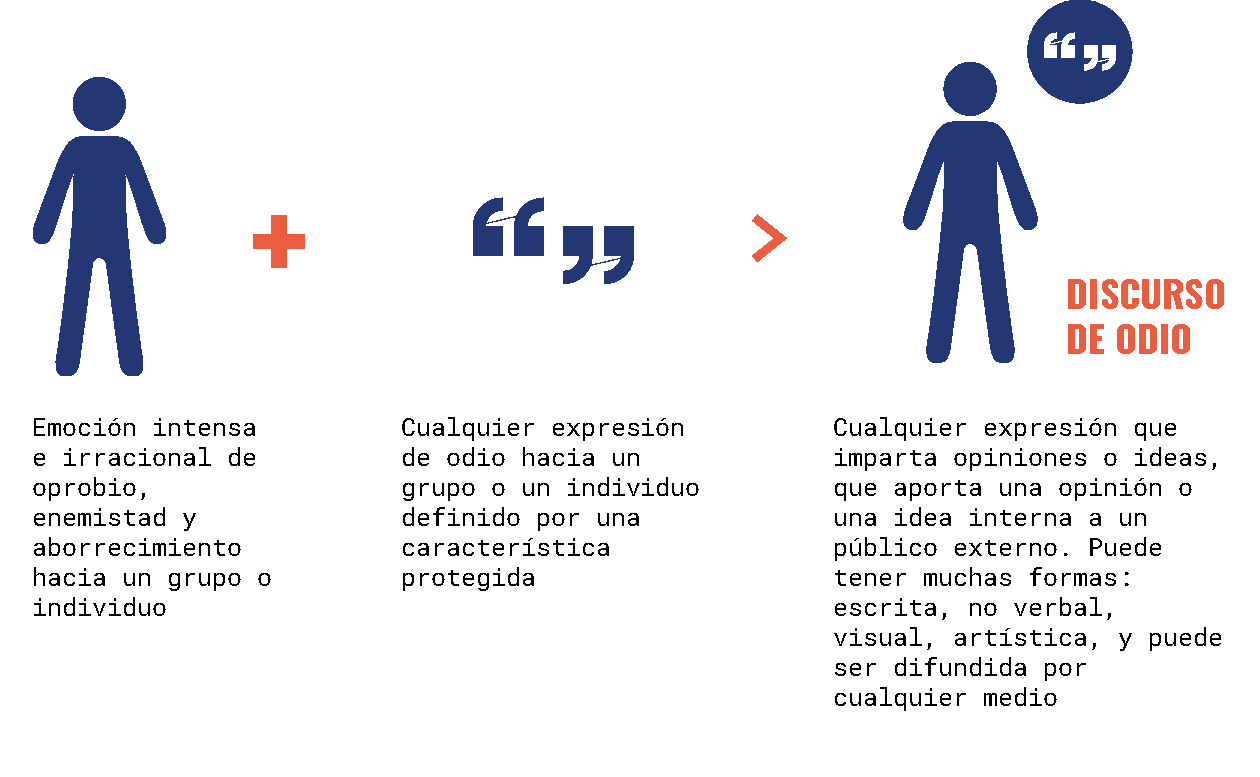
\includegraphics[width=\textwidth]{img/discurso_de_odio.pdf}
    \caption{Definición de discurso de odio de acuerdo al Toolkit de Article 19}
    \label{fig:hate_speech_definition_article_19}
\end{figure}


Entonces, puede entenderse como un discurso de cierta intensidad e irracionalidad que ataca a una persona o un grupo de personas por alguna característica históricamente vulnerada: por ser mujer, por su etnia, nacionalidad, religión, idioma, etc. La clave está en la combinación: un discurso irracional e intenso contra alguien que no posea una característica protegida no configura discurso de odio; por ejemplo, ataques a ciertas personas por ser periodistas. La figura \ref{fig:hate_speech_definition_article_19} ilustra esta definición.

No todo ataque a un individuo o una persona de algún colectivo discriminado es discurso de odio. En particular, en \citet{CIDH2015} se menciona en base al informe de la UNESCO sobre discurso de odio \citet{gagliardone2015countering} que:

\begin{displayquote}[]
    (...) el discurso de odio no puede abarcar ideas amplias y abstractas, tales como las visiones e ideologías políticas, la fe o las creencias personales. Tampoco se refiere simplemente a un insulto, expresión injuriosa o provocadora respecto de una persona. Así definido, el discurso de odio puede ser manipulado fácilmente para abarcar expresiones que puedan ser consideradas ofensivas por otras personas, particularmente por quienes están en el poder, lo que conduce a la indebida aplicación de la ley para restringir las expresiones críticas y disidentes. Asimismo, el discurso de odio tiene que distinguirse de aquellos “crímenes de odio” que se basan en conductas expresivas, como las amenazas y la violencia sexual, y que se encuentran fuera de cualquier protección del derecho a la libertad de expresión
\end{displayquote}

Como vemos, no sólamente es difusa la frontera fijada la característica sobre qué es discurso de odio o insultos, sino que incluso también es difícil definir qué característica es protegida o no. En el siguiente capítulo hablaremos más de esto al relatar cuáles fueron usadas a la hora de anotar nuestro dataset.

Si bien, como mencionamos, en cierta legislación se diferencia entre discurso discriminatorio y discurso de odio, para los fines de este trabajo utilizaremos ambas acepciones indistintamente. Cuando haya un llamado o una incitación a la violencia o algún tipo de represalia se hará explícita esta cuestión.


\section{Trabajo previo}

En esta sección haremos una breve reseña de algunos trabajos destacados del área. Un análisis extensivo de esta disciplina escapa totalmente al alcance de este trabajo. Referimos a quien esté interesado a \citet{schmidt2017survey} y a \citet{fortuna2018survey}. Más recientemente, \citet{poletto2021resources} hace un análisis pormenorizado y actualizado de los recursos para la tarea de detección de discurso de odio.

La detección del discurso del odio es una tarea de clasificación de oraciones bastante relacionada con el análisis de sentimientos y ha sido estudiada para varias redes sociales \cite{thelwall2008social, pak2010twitter, saleem2017web}. Uno de los primeros trabajos al respecto es \citet{greevy2004classifying} usando bolsas de palabras y SMVs para detectar contenido racista en páginas web. Construyeron su dataset de manera semi-supervisada buscando sitios mediante keywords y sus links en motores de búsqueda. Siguiendo un enfoque similar, \citet{warner2012detecting} usó unigrams y clusters Brown con SVM para detectar mensajes antisemitas en Twitter.

\citet{waseem2016hateful} anotó un corpus y usó n-gramas de caracteres para detectar comentarios de odio, y \citet{badjatiya2017deep} usó el mismo conjunto de datos para entrenar modelos de aprendizaje profundo e incrustaciones ajustadas junto con Gradient Boosted Trees. \citet {zhang2018detecting} entrenó una red neuronal profunda que combina CNN con unidades recurrentes cerradas \cite{cho2014learning}, superando a los sistemas anteriores en varios conjuntos de datos.

\citet{anzovino2018automatic} recopiló un corpus de tweets misóginos y propuso una taxonomía para distinguirlos en diferentes categorías. Los autores propusieron una serie de técnicas diferentes para clasificarlos, mostrando que enfoques simples (como el uso de modelos lineales junto con n-gramas de token) logran un rendimiento competitivo en conjuntos de datos de pequeño tamaño.

En cuanto a las tareas compartidas, \citet{fersini2018overview} presentó un desafío en la detección de misoginia en Twitter, tanto en español como en inglés, mientras que \citet{fersini2018evalitaoverview} planteó un desafío similar pero en italiano e inglés. \citet{bosco2018overview} propuso un concurso de detección automática sobre publicaciones de Twitter y comentarios de Facebook, que incluía discursos de odio en general.



\section{Datasets}

En esta sección haremos un recuento de los conjuntos de datos para la detección de lenguaje odioso.
\citet{nobata2016abusive} fue uno de los primeros datasets => mencionar sus criterios, y su experimento (muy interesante) de Turkers vs anotadores in-house

% \begin{table*}
%     \centering
%     \begin{tabular*}

%     \end{tabular*}
% \end{table*}

\citet{gao2018detecting}

\subsection{Criterios de anotación}

\begin{table*}[t]
    \centering
    \begin{tabular}{p{0.20\linewidth}  p{0.80\linewidth}}
        \textbf{Hate Speech} & Language which attacks or demeans a group based on race, ethnic origin, religion, disability, gender, age, disability,
        or sexual orientation/gender identity. Some examples:
        \begin{itemize}
            \item The JEWZ are Market Manipulators Hate them freaking Jews !! To bad Hitler did not finish them off !!!
            \item  I hate the mall because there are too many unemployed apefricans and mudsharks.
            \item 300 missiles are cool! Love to see um launched into TelAviv! Kill all the gays there!
            \item EGYPTIANS ARE DESCENDED FROM APES AND PIGS. NUKE EGYPT NOW Ah me tu se ku sh
        \end{itemize} \\

        \hline

        \textbf{Derogatory} & Language which attacks an individual or a group, but which is not hate speech. Some examples:
        \begin{itemize}
            \item All you perverts (other than me) who posted today, needs to leave the O Board. Dfasdfdasfadfs
            \item yikes...another republiCUNT weighs in....
        \end{itemize} \\

        \hline

        \textbf{Profanity} & Language which contains sexual remarks or profanity. Some examples:

        \begin{itemize}
            \item T.Boone Pickens needs to take a minimum wage job in FL for a week. I guarantee he shuts the f up after that.
            \item Somebody told me that Little Debbie likes to take it up the A.\$.\$.
            \item So if the pre market is any indication Kind of like the bloody red tampons that you to suck on all day??
        \end{itemize}
         \\
    \end{tabular}
    \caption{Annotation guidelines used in \cite{nobata2016abusive}}

    \label{tab:nobata_guidelines}
\end{table*}

\todo{Mandar esto al siguiente capítulo}

\section{Dataset}

\begin{table}[t]
    \centering
\begin{tabular}{ll}
    Categoría  & Cantidad \\
    \hline
    No odiosos &          \\
    Odiosos    &          \\
\end{tabular}
\caption{Números del dataset de \citet{hateval2019semeval}}
\label{tab:hateval_dataset}
\end{table}

El dataset que utilizamos en este capítulo es el provisto por \citet{hateval2019semeval}. Este dataset está orientado a la detección de discurso de odio contra mujeres e inmigrantes en Twitter, tanto en inglés como en español. Nuestro trabajo estará centrado en el dataset en español.

Posee las siguientes etiquetas:

\begin{itemize}
    \item \textbf{HS}: una etiqueta binaria que marca si el tweet tiene contenido discriminatorio (0 si no lo tiene, 1 si hay discurso de odio)
    \item \textbf{Target}: Si hay HS, una etiqueta binaria que marca si el objetivo del discurso de odio es un objetivo genérico (0) o si se refiere a un individuo específico (1)
    \item \textbf{Agresividad}: Si hay HS, una etiqueta binaria que marca si el tweet es agresivo
\end{itemize}


La tabla \ref{tab:hateval_dataset} posee los números del dataset. La tabla ZZZ posee algunos ejemplos para cada una de las características en cuestión.

\section{Tareas de clasificación propuestas}

Sobre el dataset de hatEval, los autores propusieron dos tareas:

\newcommand{\subtaska}[0]{\textbf{Tarea A}}
\newcommand{\subtaskb}[0]{\textbf{Tarea B}}

\begin{itemize}
    \item \subtaska{}: Dado un tweet predecir si contiene discurso de odio contra mujeres o inmigrantes (HS)
    \item \subtaskb{}: Dado un tweet, predecir si contiene discurso de odio (HS), si está dirigido contra un individuo o un grupo (TR), y si es agresivo o no (AG)
\end{itemize}

\todo{Pensar algún nombre mejor?}

La primer tarea es la versión clásica de la detección de discurso de odio, donde predecimos una etiqueta binaria. La segunda es una versión más rica, de grano fino, donde predecimos varias características de particular interés para distinguir algunas formas potencialmente más peligrosas de este fenómeno.

La performance de \subtaska{} es medida mediante la Macro F1 de la clase positiva y negativa. En el caso de \subtaskb{}, se mide por la Macro F1 de las 3 clases (HS, TR, AG) y también por la medida Exact Match Ratio

\begin{equation*}
    EMR = \frac{1}{n} \sum\limits_{i=1}^{n} I(Y_i, Y_i^*)
\end{equation*}

siendo $Y_i$ las etiquetas respectivas $(HS, TR, AG)$, $Y_i^*$ las etiquetas que predice nuestro sistema, e  $I$ la función indicadora ($I(x, x) = 1$, $0$ en cualquier otro caso). Observado más de cerca, esto puede entenderse la accuracy sobre la 3-upla de la salida de los clasificadores, pero usamos la terminología de Exact Match Ratio como se usa en \citet{zhang-2014-multilabel} para referirse a esta métrica (a diferencia del Hamming Score).

\section{Método}

\subsection {Preprocesamiento}


\newcommand{\elmo}[0]{ELMo}
\newcommand{\elmomodel}[0]{\emph{LSTM-\elmo{}}}
\newcommand{\bow}[0]{BoW}
\newcommand{\boc}[0]{BoC}
\newcommand{\elmobowmodel}[0]{\emph{LSTM-\elmo{}+\bow{}}}
\newcommand{\svmmodel}[0]{$\mathrm{SVM}_0$}
\newcommand{\hateval}[0]{HatEval}
\newcommand{\semeval}[0]{SemEval-2019}
\newcommand{\fasttext}[0]{\emph{fastText}}

El preprocesamiento es crucial en las aplicaciones de PNL, especialmente cuando se trabaja con datos ruidosos generados por el usuario. Aquí, seguimos \citet{atalaya_tass2018}, definiendo dos niveles de preprocesamiento: preprocesamiento básico y orientado a sentimientos. Usamos uno u otro, dependiendo de la configuración.

El preprocesamiento básico de tweets incluye tokenización, reemplazo de identificadores, URL y correos electrónicos, y acortamiento de letras repetidas.

El preprocesamiento orientado a sentimientos incluye minúsculas, eliminación de puntuación, palabras vacías y números, lematización (usando TreeTagger \cite{schmid95}) y manejo de negación.
Para el manejo de la negación, seguimos un enfoque simple:
% \cite {das01, pang02}:
Buscamos palabras de negación y agregamos el prefijo 'NOT \_' a los siguientes tokens. Se niegan hasta tres tokens, o menos si se encuentra un token que no sea una palabra.

\section{Técnicas de clasificación}

Para capturar esta información, consideramos una representación de bolsa de caracteres que codifica recuentos de caracteres $n$ -gramas para algunos valores de $ n $. Estos vectores se calculan a partir de textos originales de tweets, sin ningún procesamiento previo. \boc {} s tienen las mismas variantes y parámetros que \bow {} s.


\subsection {Word-embeddings}

Usamos \fasttext{}, una biblioteca de embeddings basada en combinaciones lineales de sub n-gramas \cite{bojanowski16} para obtener representaciones de palabras independientes del contexto.


De la misma manera que en la anterior sección, en lugar de usar vectores previamente entrenados disponibles públicamente, entrenamos nuestras propias incrustaciones en un conjunto de datos de $ \sim90 $ millones de tweets de varios países de habla hispana.
Preparamos dos versiones de los datos: una usando solo preprocesamiento básico y la otra usando preprocesamiento orientado a sentimientos (con la excepción de la lematización). Para estos dos conjuntos de datos, las incrustaciones de omisión de gramática se entrenaron utilizando diferentes configuraciones de parámetros, incluyendo una serie de dimensiones, tamaño de n-gramas de palabras y subpalabras, y tamaño de la ventana de contexto.

\subsection{Tweet Embeddings}
\label{sec:sif}

%%
%%
%%
%%  https://docs.google.com/drawings/d/1BU3ulBiqU0NojpW6Fkb4xFlMCDigSWwfjN7z9smO6nY/edit
%%
%%

\begin{figure}[t]
    \centering
    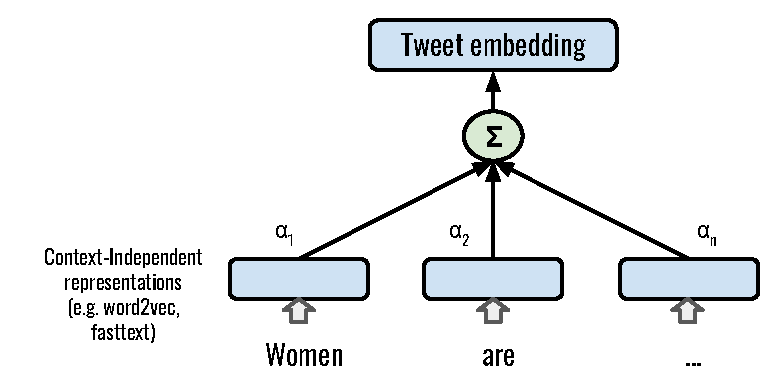
\includegraphics[width=\textwidth]{img/tweet_embeddings.pdf}
    \caption{Muestra de la recolección de datos}
    \label{fig:tweet_embeddings}
\end{figure}

Una forma relativamente simple de obtener una representación de una oración es realizar una combinación lineal de las representaciones obtenidas para cada palabra. Es decir, dada una oración $s = w_1 w_2 \ldots w_n$, y representaciones $\overline{w_1}, \overline{w_2}, \ldots, \overline{w_n} \in \mathbb{R}^m$, podemos obtener una representación

\begin{equation}
    \overline{s} = \sum\limits_{i=1}^{n} \alpha_i \overline{w_i}
\end{equation}

con $\alpha_1, \ldots, \alpha_n \in \mathbb{R}$ escalares (dependientes de la oración). De esta manera, obtenemos de $n$ representaciones independientes del contexto una representación para el tweet, sin tener en cuenta posibles interacciones entre los distintos componentes. La figura \ref{fig:tweet_embeddings} ilustra esta metodología simple para obtener representaciones de oraciones.

Tenemos entonces dos posibilidades para determinar la combinación lineal: la forma de obtener las representaciones, y la forma de calcular los coeficientes. Para las representaciones, podemos usar varias de las técnicas que ya vimos como word2vec, GloVe, o \fasttext{}. Para calcular los coeficientes, consideramos en nuestro trabajo dos formas. La primera, la forma canónica, calculando un promedio de las representaciones, es decir, tomando $\alpha_i = \frac{1}{n}$

Se utilizaron combinaciones lineales para calcular una representación de un solo tweet.
Seguimos dos enfoques simples: promedio simple y promedio ponderado. En el segundo caso, utilizamos un esquema que se asemeja a la frecuencia inversa suave (SIF) \cite {arora17}, inspirado en la reponderación de TF-IDF.
Cada palabra $ w $ se pondera con $ \frac {a} {a + p (w)} $, donde $ p (w) $ es la palabra probabilidad unigrama y $ a $ es un hiperparámetro de suavizado.
Los valores altos de $ a $ significan más suavizado hacia el promedio simple.

% También consideramos dos opciones que afectan las incrustaciones de tweets: binarización, que ignora las repeticiones de tokens en los tweets; y normalización, que escalas dando como resultado que los vectores de tweets tengan una norma unitaria.


\subsection{Embeddings contextualizados}
\label{subsec:elmo}

Después del gran salto adelante que representó las incrustaciones de palabras independientes del contexto, llegó una nueva ola en los últimos años. En lugar de tener vectores entrenados para cada palabra, se generan representaciones dependientes del contexto para cada token dada una oración. Por ejemplo, \citet{mccann2017learned} usó un codificador LSTM profundo para traducción automática para generar vectores sensibles al contexto.

\elmo{} \cite{peters2018} es uno de estos enfoques dependientes del contexto y se basa en un modelo de lenguaje bidireccional profundo (biLM). La arquitectura del modelo de lenguaje consta de L capas de LSTM bidireccionales, además de una representación de token independiente del contexto. Por lo tanto, para cada token en una secuencia, obtenemos representaciones vectoriales de $ 2L + 1 $.
% Estas representaciones se consideran profundas ya que utilizan la salida de cada capa LSTM.
Para obtener un vector final para cada token, los autores sugieren colapsar las capas en vectores mediante una combinación lineal.

% Sea $ t_1, \ldots, t_n $ una secuencia de tokens, y sea $ h_ {k, j} $ el vector que representa la salida de la capa $ j $ cuando se consume el token $ t_k $. Entonces, el vector contextualizado para el token $ k $ es:
%
% \begin {ecuación}
% ELMo_k ^ {tarea} = \gamma ^ {tarea} \sum_ {j = 0} ^ {L} s_j h_ {k, j} \label {eq: elmo}
% \end {ecuación}

En este trabajo, usamos la implementación y los modelos entrenados previamente de \cite{che-EtAl:2018:K18-2}. El modelo español se entrenó con $L = 2 $ capas y 1024 dimensiones, y la combinación lineal se realizó utilizando un promedio simple.

\subsection{Modelos}

Para las tareas propuestas, analizamos el desempeño de diversos modelos de clasificación. Algunos de ellos son los presentados para la shared-task \hateval{}, a las cuales agregamos modelos basados en transformers. Estos modelos no estaban disponibles al momento de presentar dicho trabajo. \footnote{El trabajo de BERT\cite{devlin2018bert} es de finales de 2018, y hasta finales de 2019 no fue publicada una versión entrenada en español, BETO}.

Para la tarea de detección binaria (\subtaska{}) planteamos 3 tipos de clasificadores:

\begin{itemize}
    \item Modelos lineales: regresiones logísticas y SVM con kernel lineales, consumiendo como entrada bolsas de palabras, bolsas de caracteres, y tweet embeddings usando SIF.
    \item Redes neuronales recurrentes: usando como entrada word-embeddings y embeddings contextualizados (\elmo{})
    \item BERT: Usamos la versión en español entrenada por \citet{canete2020spanish}, BETO.
\end{itemize}

Para el caso de la tarea de multidetección (\subtaskb{}), podemos pensar este problema de dos maneras:

\begin{enumerate}
    \item Un problema de clasificación múltiple
    \item Un problema de clasificación de 5 clases
\end{enumerate}

En el primer caso, el enfoque sería predecir por separado HS, AG, y TR. La segunda formulación se basa en observar que no todas las 8 combinaciones son permitidas, sino sólo 5: si no hay HS no nos interesa observar las otras dos variables. Tenemos entonces 5 clases a predecir.

Con esta última observación, propusimos en \citet{atalaya_tass2018} un modelo basado en SVM (consumiendo la misma entrada que detallamos anteriormente). No evaluamos en dicho trabajo un modelo recurrente con este esquema de clasificación, ni tampoco lo haremos aquí, considerando que evaluaremos modelos que han demostrado tener mejor performance para numerosas tareas de clasificación de texto.

Así mismo, proponemos para esta subtarea modelos basados en transformers basado en multi-clasificación. La arquitectura usual de modelos basados en BERT para clasificación constan de poner como última capa una  ``cabeza'' que consume la salida del token \verb|[CLS]|. En términos concretos, esto agrega una matriz de parámetros $W \in \mathbb{R}^{m \times 768}$ donde $m$ es la cantidad de clases de nuestro problema y 768 corresponde a la dimensión de cada vector del modelo de transformers, y usando softmax como función de activación.

Para construir un modelo de multi-clasificación, mantenemos la misma arquitectura pero, en lugar de usar como activación la función softmax, utilizamos la función sigmoidea elemento a elemento. En el caso de clasificación de $n$ clases, $softmax(W x + b)$ nos da para el elemento i-ésimo el score de que la instancia pertenezca a la clase $i$. Por otro lado, en el caso de multiclasificación de $n$ variables, $\sigma(W x + b)$ nos da el score de predecir la etiqueta positiva para el (en nuestro caso,  $\sigma(W x + b)_1$ nos da la probabilidad de que $HS = 1$,  $\sigma(W x + b)_2$ nos da la probabilidad de que $HS = 2$, etc).

Para entrenar el modelo de clasificación, evaluamos dos tipos de funciones de costo. En primer lugar, utilizamos la suma o promedio\footnote{Es equivalente optimizar una u otra} de las entropías cruzadas binarias. Concretamente, si $y = (y_{HS}, y_{TR}, y_{AG})$ son las etiquetas de una instancia e $\widehat{y}$ la predicción del modelo, la pérdida es:

\begin{equation}
\label{eq:multi_loss}
L(y, \widehat{y}) = \sum\limits_{k \in \{HS, TR, AG\}} J(y_k, \widehat{y_k})
\end{equation}

donde $J$ es la entropía cruzada. Esta función de pérdida, sin embargo, ignora cualquier tipo de jerarquía entre las variables; por ejemplo, si para una instancia tenemos $HS = 0$, toma la pérdida de las variables $TR$ y $AG$. Contemplamos entonces una variante de esta función para tener en cuenta esta jerarquía:

\begin{equation}
    \label{eq:hierarchical_loss}
    L(y, \widehat{y}) =  J(y_{HS}, \widehat{y_{HS}}) + \beta(y_{HS})\sum\limits_{k \in \{TR, AG\}} J(y_k, \widehat{y_k})
\end{equation}

donde $\beta(y_{HS})$ pondera la pérdida de las variables del segundo nivel de nuestra jerarquía. Una opción puede ser considerar $\beta(1) = 1, \beta(0) = 0$, donde ignoramos las pérdidas de las variables $TR, AG$ cuando no hay discurso discriminatorio. Análogamente, $\beta(y) = 1$ sería el caso descripto en la ecuación \ref{eq:multiloss}.

Para generalizar esto, podemos agregar un hiperparámetro $\gamma \in [0, 1]$ para escribir $\beta(y) = (1-y) \gamma + y$.


\section{Resultados}

\newcommand{\mr}[2]{\multirow{#1}{*}{#2}}
\newcommand{\esrow}[1]{\multirow{#1}{*}{es}}
\newcommand{\enrow}[1]{\multirow{#1}{*}{en}}
\newcommand{\tbf}[1]{\textbf{#1}}


\begin{table}

    \centering

    \begin{tabular}{l l| l l l}
        Modelo       & Idioma              & Recall     & Precision & Macro-F1 \\
        \hline
        SVM          & \mr{3}{es}          & Recall     & Precision & 0.730    \\
        ELMO-RNN     &                     & 0.753      & 0.669     & 0.735    \\
        BETO         &                     & 0.839      & 0.674     & 0.764    \\
        \hline
        ELMO-RNN     & \mr{4}{en}          & ?          & ?         & 0.471   \\
        BERT         &                     & 0.968      & 0.474     & 0.496   \\
        RoBERTa      &                     & 0.967      & 0.470     & 0.485   \\
        BERTweet     &                     & 0.958      & 0.495     & 0.546
    \end{tabular}
    \caption{Resultados de la evaluación para la detección de discurso de odio en datasets de desarrollo y test, medidas por la métrica macro F1. En negrita, el mejor resultado.}
    \label{tab:hateval_task_a}
\end{table}



La tabla \ref{tab:hateval_task_a} muestra los resultados de evaluación para los modelos propuestos para la detección de discurso de odio ``plana''. Marcamos con un asterisco aquellos modelos presentados en \citet{atalaya_tass2018}. Respecto a los resultados en español, podemos observar que entre los presentados para aquella competencia, el modelo basado en SVMs obtiene la mejor performance, aún contra aquel basado en embeddings contextualizados, obteniendo el mejor desempeño en dicha con $0.730$ de Macro F1. La pobre performance de ELMo contra un modelo mucho más simple puede deberse a un mal entrenamiento , y puede que también debido al cambio de dominio, contra los cuales la entrada de las SVM está mejor adaptada.

Para ambos idiomas, los modelos basados en transformers \cite{vaswani2017attention} obtienen la mejor performance, con considerables mejoras respecto a los modelos basados en ELMo (y a los SVMs en el caso del español). Particularmente, en el caso del inglés, BERTweet \cite{bertweet} obtiene la mejor Macro-F1. En el capítulo 7 presentaremos un modelo similar a BERTweet para español que mejora la performance sobre BETO, a la vez que evaluaremos sobre versiones de BETO ajustadas al dominio social\footnote{Un modelo que no evaluamos en el presente trabajo es la versión en español de RoBERTa, recientemente entrenada. En el capítulo 7 evaluaremos su performance}.

La tabla \ref{tab:hateval_task_b} muestra los resultados de la \subtaskb{}, reportado por las F1 de cada variable predicha (HS, TR, AG), así como por el Macro F1 de HS y el Macro F1 de las 3 variables mencionadas. Los resultados están expresados como la media de 10 corridas independientes del experimento para cada configuración distinta. Consideramos las 3 versiones: Multi refiere a clasificación múltiple, Jerárquica a clasificación múltiple con la función de costo jerárquica, y Combinatoria a la conversión del problema en una clasificación de 5 clases.

Podemos observar que para español, la mejor performance en términos de EMR (la métrica más estricta) es el clasificador entrenada con la función de costo definida en \ref{eq:hierarchical_loss} (con el hiperparámetro $\gamma = 0.1$); sin embargo, esta diferencia la diferencia entre las performances no es significativa al correr un test de Kruskal-Wallis ($H(9) = 3.492, p = 0.174$). En términos de Macro-F1, la mejor performance es de BETO con el problema de clasificación múltiple y sin la función de costo jerárquica, pero de nuevo esta diferencia no es significativa ($H(9) = 3.656, p=0.16$).

Respecto al inglés, los mejores resultados pueden observarse en el modelo entrenado con BERTweet con la salida de 5 clases. Este resultado, sin embargo, queda en términos de EMR por debajo del baseline, y contemplando el Macro F1 de los mejores resultados de la competencia, obtenidos por el equipo MITRE \cite{gertner-etal-2019-mitre}. En ese trabajo se basaron en un ensemble de modelos entrenados con BERT, usando también un ajuste de dominio sobre tweets. Esta baja performance de nuestros modelos (y de los modelos en general sobre ese dataset) puede deberse a problemas de anotación y de que las particiones de train y test no son idénticamente distribuid

Algo que puede observarse es que, lejos de dañarse la performance de la detección de lenguaje discriminatorio (lo que analizamos en la \subtaska{}), predecir varias variables pareciera mejorar la performance. Este resultado puede verse en ambos idiomas, obteniendo cerca de (+1 puntos de Macro F1, y cerca de +4 puntos Macro F1 en inglés). \todo{Correr un test estadístico para ver si esto es significativo}.



\begin{table}
    \small
    \centering
    \begin{tabular}{lll rrr rrr}
        Modelo            & Salida         & Idioma     &  HS F1     & TR F1        &  AG F1        &   EMR       &  Macro F1       & Macro HS F1 \\
        \mr{3}{beto}      & multi         & \mr{3}{es}  &  0.741     &  \tbf{0.765} &  \tbf{0.688}  & 0.685       &     \tbf{0.731} &  0.771      \\
                          & jerárquico    &             &  0.735     &  0.758       &  0.674        & \tbf{0.703} &     0.722       &  0.776      \\
                          & combinatoria  &             &  \tbf{742} &  0.763       &  0.668        & 0.698       &     0.724       &  0.776      \\

        \hline
        \mr{3}{BERT}      & multi         & \mr{3}{en}  &  0.638     &  0.600       &  0.443        & 0.380       &     0.560       &  0.512      \\
                          & jerárquico    &             &  0.642     &  0.592       &  0.451        & 0.388       &     0.562       &  0.521      \\
                          & combinatoria  &             &  0.644     &  0.593       &  0.442        & 0.398       &     0.560       &  0.531      \\
        \mr{3}{BERTweet}  & multi         &\mr{3}{en}   &  0.658     &  0.629       &  0.462        & 0.426       &     0.583       &  0.567      \\
                          & jerárquico    &             &  0.656     &  0.617       &  0.450        & 0.423       &     0.574       &  0.555      \\
                          & combinatoria  &             &  0.666     &  0.637       &  0.444        & 0.449       &     0.582       &  0.589      \\
    \end{tabular}

    \caption{Resultados de la evaluación para la detección de discurso múltiple de discurso de odio, \subtaskb{}, en términos de las F1 de las clases HS (Hate Speech), TR (Targeted), AG (Aggressive), el Exact Match Ratio (EMR), las Macro F1 de las clases en cuestión, y la Macro F1 de la clase HS.  }
    \label{tab:hateval_task_b}
\end{table}




\subsection{Análisis de Error}

Analizamos los errores sólo para el dataset en español. Para ello, tomamos las predicciones de 10 clasificadores BERT, y observamos qué instancias son repetidamente clasificadas erróneamente por los modelos, para así sortear la alta variabilidad de estos.

\section{Discusión}


\subsection{Problemas de anotación}

\subsection{Falta de contexto}

Un problema que observamos en el dataset estudiado en este capítulo (pero que aplica a otros también) es la falta de contexto: muchos de los mensajes carecen de información adicional sobre la noticia o el tema del que se está hablando. Cuando leemos un mensaje de un tweet, casi siempre los leemos en el contexto de una noticia, o un trending topic. Muy rara vez leemos un mensaje en total aislamiento \todo{podemos justificar un poco más esto?}.

Más aún, un género no explorado en estos mensajes (usualmente aislados) son aquellos en los cuales el contexto es necesario para extraer un significado. Por ejemplo, un comentario que dice ``hay que matarlos'' puede o no entenderse como discurso de odio. Si el objeto del mensaje se refiere a mosquitos, ese mensaje no es odioso; si, por otro lado, está hablando sobre chinos en el contexto del COVID-19, entonces ese mensaje es discriminatorio (y además llama a tomar una medida violenta).

En ese sentido, podemos preguntarnos sobre este punto es si el acceso a información contextual nos puede auxiliar en la detección de discurso de odio. Por ejemplo, tener acceso a una noticia, al hilo de conversación

\todo{¿Quizás falta también algo más a nivel semiótico acá?}

\subsection{Interpretabilidad y fragilidad de clasificadores}

\section{Conclusiones}

En este capítulo hemos hecho una primer acercamiento a la tarea de detección de lenguaje discriminatorio, haciendo un repaso de su definición desde una perspectiva legal y social\todo{?}, así como también desde una perspectiva técnica analizando técnicas de clasificación usando el dataset presentado en la shared task multilingual \emph{hatEval}\cite{hateval2019semeval}. En base a este dataset, analizamos dos tareas: detección binaria de discurso de odio, y detección de múltiples variables (si es discurso de odio, si es dirigido, si es agresivo).

Para estas tareas, presentamos varios modelos de clasificación. Por un lado, clasificadores lineales que consumen distintos tipos de entrada como ser tweet embeddings y bolsas de caracteres; modelos recurrentes que consumen embeddings contextualizados; y finalmente, modelos del estado del arte basados en modelos de lenguaje pre-entrenados usando la arquitectura de transformers. Para ambas, los modelos de transformers

En el caso de la tarea de detección múltiple, propusimos dos formas de atacar el problema: como clasificación múltiple (prediciendo simultáneamente las 3 variables), y convirtiendo a un problema de clasificación simple sobre 5 clases posibles. Observamos, a su vez, que lejos de dañar la performance de la detección de discurso de odio, predecir más de una variable mejora la performance de nuestros clasificadores.

Analizando este dataset y algunos otros de la bibliografía, marcamos algunas puntos de mejora en la detección de discurso de odio: principalmente, la falta de información contextual. La mayoría de los datasets no tienen mayor información sobre los mensajes de los usuarios, algo que usualmente no pasa en las redes sociales. Por otro lado, y teniendo en cuenta la observación hecha en el párrafo anterior, nos preguntamos si tener información más granular acerca de las características . Finalmente, observamos que para la creación de datasets de un fenómeno tan complejo y social es indispensable tener muchos recaudos a la hora de la anotación, algo que ya ha sido observado en otros trabajos \todo{Citar trabajo sobre la performance de entrenar sobre datos de crowdsource vs etiquetadores especializados}.

En los siguientes capítulos, exploraremos algunas de estas observaciones. Particularmente, nos centraremos en la incorporación de contexto en la detección de discurso discriminatorio, construyendo un dataset que incorpore esta información a los mensajes anotados. Luego de eso, abordaremos la pregunta ¿puede el contexto de un mensaje ayudar a mejorar la detección de discurso de odio?

% \chapter{Limitaciones de todo: metodológicos, de los corpus, de los modelos.}
% \section{Anotación y sus limitaciones}

\section{Falta de contexto}

Citar paper

\section{Interpretabilidad y fragilidad de clasificadores}
\part{Creación del dataset}

\chapter{Metodología y definiciones}
\label{chap:dataset_creation}

En este capítulo contaremos el diseño del proceso de recolección, selección y anotación de datos. Por lo marcado en anteriores secciones, consideramos interesante el problema de hacer una detección de lenguaje discriminatorio bajo un contexto. Es decir, no es lo mismo considerar el mensaje ``sos un hombre'' en solitario que si ese mismo mensaje está dirigido hacia una mujer trans.

Nos abocamos a la decisión de crear un dataset que no sólo contenga un mensaje/comentario, sino que provea un contexto en el cual se da este mensaje. Un ámbito natural para esta tarea son las notas periodísticas, donde disponemos de una nota y comentarios realizados sobre esta. Un ejemplo puede verse .

Muchos sitios de noticias disponen de sistemas embebidos de comentarios, pero vista la dificultad para la recolección a la vez que los limitados datos provistos por estos sitios nos llevaron a buscar otro medio: Twitter. Twitter provee una sencilla API para descargar datos, a la vez

Algo a tener en cuenta es que este tipo de datos tiene una naturaleza particular, ya que las agresiones discriminatorias son usualmente a personajes públicos o colectivos de personas, y se dan de manera indirecta (a través del comentario en la noticia) y no directa (es decir, como respuesta al usuario de Twitter ofendido)

\section{Trabajos previos}
\label{sec:dataset_previous}

Pocos trabajos incorporan algún tipo de contexto a los comentarios del usuario para estas tareas. \citet{gao-huang-2017-detecting} construyó un dataset de lenguaje discriminatorio sobre 1518 comentarios del sitio de Fox News. A los anotadores les fue presentado tanto el comentario como la noticia a la hora de realizar el etiquetado. Sobre este dataset, efectuó experimentos de clasificación usando modelos lineales (regresiones logísticas) y modelos neuronales. En estos experimentos observó que un clasificador (tanto lineal como neuronal) mejora su performance al consumir el título de la noticia, dando indicios de que se puede aprovechar el contexto para mejorar la detección de este fenómeno. Sin embargo, como marca \citet{pavlopoulos2020toxicity} este trabajo cuenta con algunos problemas: en primer lugar, el tamaño del dataset es pequeño, y está extraído de sólo 10 noticias, lo cual limita los posibles contextos. A su vez, la anotación fue realizada mayormente por un único anotador, lo cual hace poco confiables las etiquetas. Luego, algunos detalles menores debieran ser analizados con mayor detalle, como por ejemplo la utilización de los nombres de usuarios como features predictivas.

\citet{mubarak-etal-2017-abusive} construyó un dataset en árabe sobre comentarios con contenido abusivo del portal Al Jazeera. Sin embargo, este daaset tiene un problema: los comentarios son sólo presentados a los anotadores sobre noticias, ignorando todo el thread de la conversación. Esto hace que el contexto sea parcial.


Paralelamente a nuestro trabajo, \citet{pavlopoulos2020toxicity} analiza el impacto de agregar contexto a la tarea de detección de toxicidad. En particular, plantea dos preguntas

\begin{itemize}
    \item ¿Qué tanto afecta el contexto a la toxicidad percibida por humanos en conversaciones online?
    \item ¿Puede el contexto ayudar a mejorar la performance de clasificadores de toxicidad en comentarios?
\end{itemize}

Para responder estas preguntas, los autores construyeron dos datasets en base a Wikipedia Talk Pages\cite{hua-etal-2018-wikiconv}, un dataset de discusiones del sitio de Wikipedia. En primer lugar, armaron un dataset de 250 comentarios anotados por dos grupos disjuntos de anotadores: uno de los grupos anotó los comentarios de manera contextualizada, viendo tanto el comentario en cuestión como el título de la discusión; el otro grupo sólo vio el comentario a anotar sin contexto alguno. En dicho experimento observaron que los anotadores contextualizados percibieron 6.4\% de comentarios tóxicos versus un 4.4\% de quienes anotaron sin contexto, una diferencia significativa aplicando un test Mann-Whitney. Desagregando estos resultados, observaron que 13 de los 250 comentarios (5.2\%) tuvieron diferencias de anotación entre los dos grupos, con 9 (3.6\%) comentarios donde aumentó la toxicidad percibida y 4 comentarios donde bajó la toxicidad al ser agregado el contexto.

Para responder la segunda pregunta, anotaron un dataset de 20k comentarios, 10k anotados por un grupo que etiquetó viendo el contexto y otros 10k que no lo vio. Entre todos los comentarios del dataset original de Wikipedia Talk Pages, eligieron aquellos con profundidad entre 2 (respuestas directas) a 5, y con entre 10 y 400 caracteres de largo. Luego, entrenaron varios clasificadores usando este dataset y allí pudieron observar que el contexto no pareciera mejorar la performance. En el próximo capítulo nos extenderemos sobre las técnicas utilizadas por este trabajo.

\citet{xenos-2021-context} continúa el trabajo de \citet{pavlopoulos2020toxicity} desagregando el resultado de la segunda pregunta. Encuentran que el contexto parece mejorar el desempeño para un subgrupo de comentarios que son más `` sensibles al contexto '', esto medido comparando la diferencia entre las anotaciones usando el contexto y no usando el contexto. \citet{sheth2021defining} señala algunas oportunidades para incorporar fuentes de información más ricas a la tarea de detección de toxicidad, como el historial de interacción entre los usuarios, el contexto social y otras bases de conocimiento externas.

Nuestra definición de discurso de odio contiene algunas formas implícitas de abuso y, en particular, marcamos las ``llamadas a la acción'', que se detallan en \citet{wiegand2021implicitly} entre otros tipos sutiles de comportamiento tóxico en las redes sociales.

\section{Recolección de noticias y comentarios}

\begin{table*}[t]
    \centering
    \begin{tabular}{ c|c|c }
        coronavirus  &  encierro          & síntomas \\
        covid        &  fase              & dengue   \\
        cuarentena   &  infectados        & aedes    \\
        normalidad   &  Wuhan             & mosquito \\
        aislamiento  &  distanciamiento   & cacharro \\
        padecimiento &  fiebre            &          \\
    \end{tabular}
    \caption{Words used to retrieve COVID-19 and Dengue related articles.\label{tab:article_words}}
\end{table*}


\todo{Explicar un poco más
qué es lo que queremos recolectar.
Poner algún gráfico de la idea}


Usamos la API de Twitter Stream mencionando cualquiera de estas cuentas. \todo{Explicar el proceso más detalladamente} Para cualquier tweet de uno de estos medios, reconstruimos la conversación. Para el propósito de este trabajo, solo estamos interesados en el primer nivel de respuestas al tweet original \footnote{Usamos una versión antigua de la API. La versión 2.0 parece facilitar la recopilación de conversaciones}. También eliminamos las URLs de los artículos de los enlaces.


Si bien consideramos otros medios (en particular, los ``periódicos'' electrónicos de derecha) decidimos apostar por medios más tradicionales con apoyo escrito: Clarín (@clarincom), La Nación (@LANACION), Infobae (@infobae), Perfil. (@perfilcom), Crónica (@cronicacom). Como el proceso de anotación iba a ser realizado por anotadores locales, decidimos no recopilar ningún dato de otros países de habla hispana.


El foco se hizo en artículos relacionados con COVID-19. Para ello, seleccionamos artículos buscando una cantidad de palabras en su cuerpo, por lo que seleccionamos específicamente artículos relacionados con COVID-19. La tabla \ref{tab: article_words} contiene las palabras utilizadas para recuperar estos artículos. También estábamos interesados en la pandemia del dengue; sin embargo, solo se recuperó un número muy pequeño de artículos.


\subsection{Diarios elegidos}

Para esta tarea, elegimos 5 diarios:

\begin{itemize}
    \item Clarín
    \item La Nación
    \item Infobae
    \item Perfil
    \item Crónica
\end{itemize}

Estos diarios son los mayores generadores de contenido. Consideramos otros medios, pero nos atuvimos a medios formales tradicionales y con soporte escrito.

En un principio consideramos la posibilidad de anotar tweets de digiarios de otros países, pero teniendo en cuenta que esta tarea depende fuertemente de la jerga y de las variaciones dialectales de cada país decidimos realizar sólo anotación de estos diarios. A su vez, observamos que la mayoría de los comentarios son de la variedad dialectal rioplatense


\subsection{Datos recolectados}

\begin{table}[t]
    \centering
    \begin{tabular}{c|c|c}
    Medio      & \#Artículos recolectados & \#Comentarios \\
    \hline
    @infobae   &  45652   &  822462 \\
    @clarincom &  29050   &  672401 \\
    @perfilcom &  8764    &  61203  \\
    @LANACION  &  16040   &  506091 \\
    @cronica   &  17250   &  70872 \\
    \hline
    Total      & 116756  & 2133029 \\
    \end{tabular}
    \caption{Artículos recoletados por medio}
    \label{tab:articulos_recoletados_por_medio}
\end{table}


En la tabla \ref{tab:articulos_recoletados_por_medio} damos los números de los artículos recolectados por cada medio, luego de aplicado . Si bien recolectamos más artículos de otros medios, no son enumerados. Infobae es el medio que más producción de artículos genera, y también será finalmente sobre el que más comentarios etiquetemos.

La figura \ref{fig:fecha_articulos_por_medio_todas} muestra la distribución temporal de los artículos, sin aplicar ningún filtro por palabras, mientras que \ref{fig:fecha_articulos_por_medio_covid} muestra aquellas relacionadas al COVID-19 utilizando el filtro de palabras listado en la tabla \ref{tab:article_words}. Podemos observar dos caídas. Hay un pequeño pozo en mayo 2020 que se debió a la caída de nuestros servidores de recolección. Por otro lado, observamos que algunos medios (particularmente La Nación) parecieran mencionar menos directamente al COVID (al menos con los términos referidos anteriormente) hasta un nuevo pico cerca de fin de año, coincidente con un nuevo rebrote del virus en este país.

Sin embargo, todo esto puede ser un artefacto del método de filtrado: muchas notas contienen links a otras con sus títulos y eso puede interferir en estas estimaciones. Así y todo, decidimos mantener este método ya que consideramos que mayormente las notas en el período referido tienen relación con la pandemia.

\begin{figure}
    \centering
    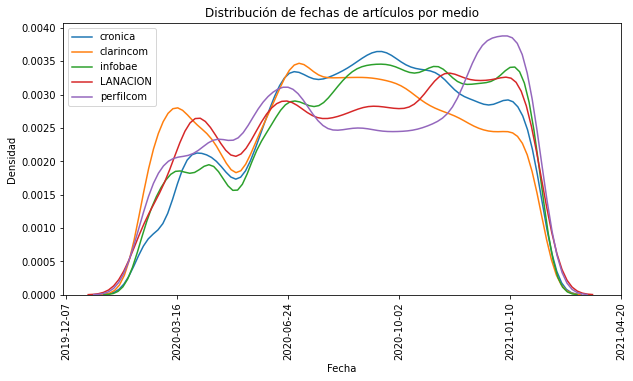
\includegraphics[width=\textwidth]{img/fechas_por_medios_todas.png}
    \caption{Distribución temporal de artículos recolectados}
    \label{fig:fecha_articulos_por_medio_todas}
\end{figure}



\begin{figure}
    \centering
    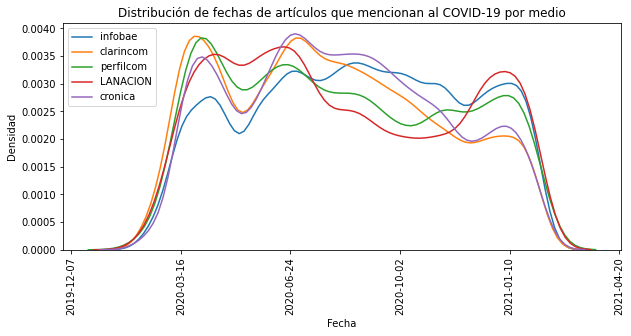
\includegraphics[width=\textwidth]{img/fechas_por_medios.png}
    \caption{Distribución temporal de artículos recolectados que mencionan COVID-19 o algún término relacionado}
    \label{fig:fecha_articulos_por_medio_covid}
\end{figure}



\section{Selección de datos a anotar}


Un problema que se nos presenta antes de comenzar el etiquetado es el de seleccionar los artículos que vamos a etiquetar. Una primera posibilidad para hacer esto es realizar una selección aleatoria de artículos y comentarios; sin embargo, los comentarios discriminatorios no se distribuyen de manera uniforme entre los artículos, sino que se concentra en algunos temas. Es mucho más probable encontrar comentarios de índole discriminatoria en notas que tengan temas cercanos a alguna de las características protegidas; por ejemplo, es esperable que encontremos contenido odioso en notas sobre China y el Coronavirus o sobre una chica transgénero antes que en un artículo de fútbol o economía.

Teniendo esto en cuenta, evaluamos varias alternativas. La primera es observar los artículos e intentar seleccionar aquellos que consideremos que puedan tener contenido potencialmente discriminatorio.

Una posibilidad para esto sería usar algunas palabras ``semilla'' para seleccionar artículos interesantes. Otra sería buscar directamente comentarios que contengan algunos insultos comunes o expresiones peyorativas hacia nuestros grupos protegidos. Después de algunos experimentos, decidimos utilizar el muestreo basado en comentarios.

\subsection{Selección en base a artículos}

En primer lugar, consideramos la posibilidad de hacer una selección en base al contenido de los artículos. Luego de realizar algunos experimentos usando LDA \cite{blei2003latent} para buscar tópicos posibles de las notas, decidimos realizar una selección un poco más controlada y determinística en base a la utilización de palabras clave. Es decir, seleccionaremos artículos en base a la aparición o no de ciertas ``semillas''

Para ello, indexamos todos nuestros artículos en MongoDB \footnote{\url{https://www.mongodb.com/}}, una base de datos no relacional y desestructurada. MongoDB permite la utilización de índices en base a texto, y realizar búsquedas en base a textos, palabras, e inflexiones. Cada artículo fue indexado en base al contenido de su cuerpo (es decir, el texto en sí del artículo).

La tabla \ref{tab:palabras_articulos} muestra el conjunto utilizado para recolectar artículos. Como vemos, hay diversas palabras que recogen distintas temáticas de posibles tópicos ``calientes'', algunos muy locales respecto a eventos concretos durante la pandemia. Si algún artículo contiene una de las frases mencionadas, se selecciona el artículo para ser etiquetado.

\begin{table}[]
    \centering
    \begin{tabular}{l | l | l | l}
    China        &  piqueteros              &  mamá                & empleadas domésticas  \\
    Cuba         &  villas                  &  de género           & la modelo             \\
    cubano       &  la villa                &  aborto              & la periodista         \\
    bolivia      &  movimientos sociales    &  actriz              & la cantante           \\
    paraguayo    &  organizaciones sociales &  actrices            & travesti              \\
    judío        &  tomas de tierras        &  feminista           & trans                 \\
    camionero    &  toma de tierras         &  femicidio           & gay                   \\
    ladrón       &  sindicatos              &  enfermera           & homosexual            \\
    represión    &  Guernica                &  madre               & de la V               \\
    criminal     &  mapuches                &  personal doméstico  & Ofelia                \\
    \end{tabular}
    \caption{Palabras utilizadas para la selección de artículos}
    \label{tab:palabras_articulos}
\end{table}

\subsection{Selección en base a comentarios}

Otra posibilidad evaluada fue la de observar los comentarios de los artículos en lugar del contenido del artículo, y seleccionarlos en base a esto. En este punto, la idea es únicamente seleccionar los artículos y no los comentarios; estos últimos son sólo usados como ``pistas'' para ver comentarios con posible contenido discriminatorio, y como tal identificar a ese artículo como un posible generador de este tipo de contenido.

La idea es similar a la de la selección con artículos, sólo que aplicada a comentarios: buscamos comentarios que contengan alguna de las palabras semilla listadas en la Tabla \ref{tab:palabras_comentarios}. Estas palabras fueron recolectadas a base de experimentación y observación de los datos, y tratan de contener diversas expresiones de contenido mayormente discriminatorio.

Una idea también considerada fue la de utilizar un clasificador entrenado sobre otro dataset (por ejemplo, el de \citet{hateval2019semeval}) y con eso marcar comentarios posiblemente discriminatorios. Sin embargo, muy probablemente detectaríamos sólo comentarios para las categorías/características etiquetadas en esos datasets e ignorarían las que agregamos en nuestro trabajo; por ejemplo, la mayoría de los datasets no contienen comentarios anotados contra la comunidad LGBTI.

El procedimiento de selección consta de, dado un artículo, marcar sus comentarios que contengan una o más de las expresiones listadas. Si el artículo tiene tres o más comentarios marcados, entonces seleccionamos el artículo; caso contrario, es descartado.

\todo{Agregar comparación con métodos de recolección en base a esto de 'seed' words}

Vale remarcar que este proceso de selección es para los \emph{artículos}, no para los comentarios.

\begin{table*}[t!]
    \centering
    \begin{tabular}{l|l|l|l|l|l|l}
    bija          & urraca     & viejo puto    & trolo      & peruano  & matarlos         & negra      \\
    prostituta    & tucán      & trabuco       & sodomita   & peruca   & una bomba        & negro de   \\
    feministas    & putita     & travesti      & chinos de  & judío    & vayan a laburar  & negros     \\
    feminazis     & reventada  & trava         & bolita     & sionista & vayan a trabajar & bala       \\
    aborteras     & marica     & degenerado    & paraguayo  & villeros & gorda            & uno menos  \\
    \end{tabular}
    \caption{Palabras utilizadas para recolectar comentarios}
    \label{tab:palabras_comentarios}
\end{table*}

Luego de algunos análisis experimentales y observacionales de las dos posibles metodologías, decidimos utilizar el muestreo de artículos en base a comentarios. En base a un análisis subjetivo, los artículos seleccionados parecían tener mayor incidencia de mensajes odiosos y eso nos decantó hacia esa opción.

\section{Criterios de anotación}
\label{sec:criterios}

La definición de lenguaje discriminatorio utilizada en este trabajo está basada en trabajos de la Comisión Interamericana de Derechos Humanos (CIDH)\cite{CIDH2015}, del Centro de Estudios de Libertad de Expresión (CELE) \cite{cele2019} y en el Article 19 Hate Speech Toolkit \cite{article192015}.

Teniendo estos insumos en cuenta, entendemos que hay discurso discriminatorio en un texto social si contiene declaraciones de carácter intenso y posiblemente irracional de rechazo, enemistad y aborrecimiento contra un individuo o contra un grupo, siendo estos objetivos de estas expresiones por poseer (o aparentar poseer) una característica protegida.

Las características en cuestión son protegidas por leyes internacionales. En este trabajo consideramos las siguientes:

\begin{enumerate}
\item Sexo (Mujeres, concretamente)
\item Género o identidad sexual (Colectivo LGBTI)
\item Ser inmigrantes, extranjeros, pueblos aborígenes u otras nacionalidades (xenofobia, racismo)
\item Situación socioeconómica o barrio de residencia
\item Poseer discapacidades, problemas salud mental o de adicción al alcohol, drogas u otros estupefacientes
\item Opinión o ideología política
\item Aspecto o edad (mayormente, gordofobia/gerontofobia)
\item Antecedentes penales o estar privado de la libertad
\end{enumerate}

Si bien algunas de estas características no son consideradas en algunos tratados (por ejemplo, contra los presos), las tuvimos en cuenta por las características propias del tratamiento en medios durante la pandemia de distintos sucesos.

\todo{Linkear el apéndice}

\section{Modelo de etiquetado}



Un modelo de anotación es, según \citet{pustejovsky2012natural}, una representación práctica del objetivo de anotación. En nuestro caso, queremos marcar comentarios discriminatorios, marcar a qué grupos y/o características se está ofendiendo, y también identificar llamados a tomar alguna acción contra los objetos de esos discursos. Por lo pronto, haremos una definición que capture ese objetivo sin deternos demasiado en especificarlo formalmente (lo que llaman en ese libro ``especificación'').

\subsection{Modelo Jerárquico de Etiquetado}



\begin{figure}
    \centering
    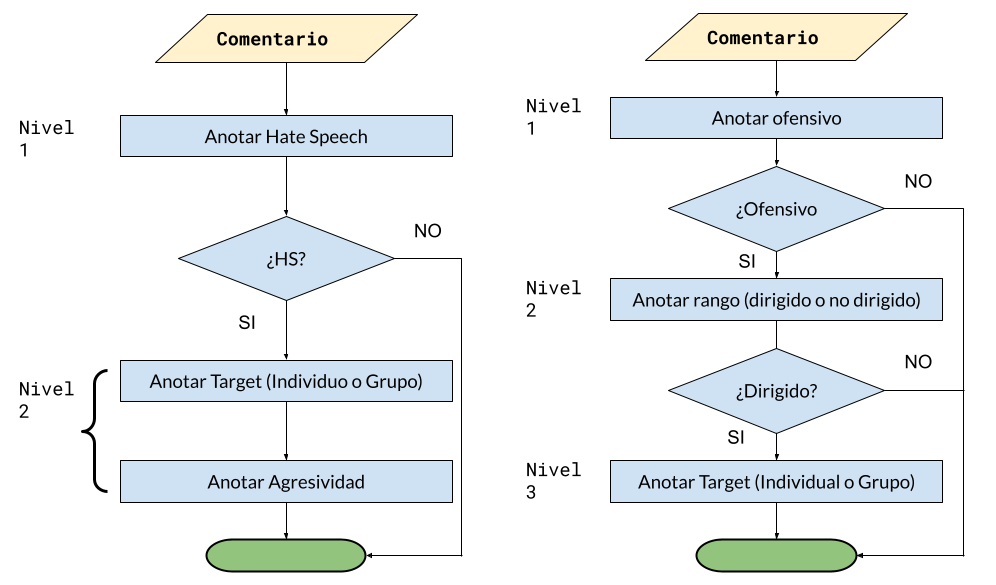
\includegraphics[width=\textwidth]{img/modelosjerarquicos.png}
    \caption{Modelos jerárquicos de anotación. A la izquierda, tenemos el modelo jerárquico propuesto para HatEval \cite{hateval2019semeval}, a la derecha el modelo propuesto para OffensEval \cite{zampieri2019semeval2019}}
    \label{fig:modelos_offenseval_hateval}
\end{figure}

\subsection{Modelo de etiquetado jerárquico y contextualizado}

\citet{zampieri2019predicting} introdujeron un modelo jerárquico de anotación para la tarea de lenguaje ofensivo, utilizado en las competiciones OffensEval \cite{zampieri2019semeval2019} y hatEval \cite{hateval2019semeval}. La idea de la anotación jerárquica es realizar anotaciones adicionales sólo para algunos casos de anotaciones del nivel anterior.

En el caso de \emph{HatEval}, tenemos un primer nivel que consta de anotar si un tweet contiene o no lenguaje de odio (nivel 1). Si el tweet tiene lenguaje de odio, entonces anotamos si está dirigido a un individuo o a un grupo, y también anotamos si es agresivo o no (ambos nivel 2). En el caso de \emph{OffensEval}, primero anotamos si es ofensivo (nivel 1), luego si está dirigido o es un insulto no dirigido (nivel 2) y finalmente, si es dirigido y ofensivo, marcamos su objetivo (nivel 3). En la figura \ref{fig:modelos_offenseval_hateval} ilustramos ambos modelos.


%
%
% Link: https://docs.google.com/drawings/d/1ZgTmvRwMWn0B-kokfw87jfSa7eY5-OSBHwltetnNT08/edit
%



\begin{figure}
    \centering
    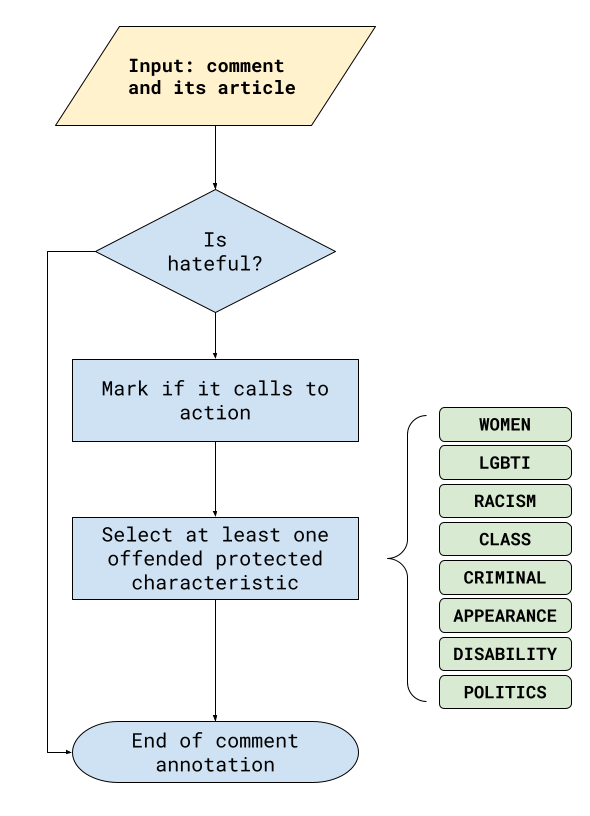
\includegraphics[width=0.5\textwidth]{img/Annotation Model.png}
    \caption{Modelo de anotación}
    \label{fig:annotation_model}
\end{figure}


La figura \ref{fig:annotation_model} muestra el modelo de anotación utilizado para el dataset construído en este trabajo. Seguimos un modelo jerárquico similar al propuesto por \citet{zampieri2019predicting}, aunque de sólo un nivel. Para cada comentario y su respectivo contexto (el artículo), requerimos una anotación  para decidir si el comentario es odioso o no. Si no es odioso, no se necesita más información. Si es así, el par artículo-comentario debe contener, además, una anotación por si llama o no a la acción, y al menos una categoría protegida





\section{Etiquetadores}

A diferencia de otros trabajos (como hatEval \cite{hateval2019semeval}), decidimos por un lado, garantizar que nuestros anotadores estén más cercanos culturalmente al problema en cuestión, a la vez que tener mayor control del perfil de estos. Consideramos que el discurso de odio tiene un fuerte componente cultural, muchas veces expresado a través de jerga o expresiones dialectales muy particulares, y relacionado con noticias muy propias de esta región.


\subsection{Tipos de anotación en otros trabajos}

Comentar otros trabajos acá

\begin{itemize}
    \item Davidson
    \item Waseem
    \item hatEval
    \item CONAN
    \item Gao (contextualizado)
    \item Context offensive (el de Google, y el griego)
\end{itemize}

\subsection{Perfil de etiquetadores}

Para la selección de anotadores, realizamos una búsqueda interna. Puntualmente, buscamos:

\begin{itemize}
    \item Estudiantes/graduades de carreras de Cs. Sociales, Psicología, Letras o afines
    \item Hablantes nativos (o casi) de Español Rioplatense
    \item Usuarios de redes sociales; preferentemente Twitter
\end{itemize}

Luego de una breve entrevista donde les contamos el proyecto y corroboramos que efectivamente sean hablantes nativos de Español Rioplatense y usuarios de RRSS, les mandamos una pequeña evaluación paga que constó de leer el manual de criterios de anotación (que agregamos en \ref{app:manual_criterios_anotacion}) y anotar 5 artículos. Esto lo realizamos para ver que efectivamente estén entendiendo la tarea. Estos artículos fueron luego reutilizados para el proceso de entrenamiento.

\section{Proceso de etiquetado}

\subsection{Preprocesado y filtrado de los datos}

El preprocesado de los datos es muy básico: en los hechos, efectuamos el mismo preprocesamiento que en anteriores tareas, consistente en reemplazar handles de Twitter por un token especial \verb|@usuario| para evitar cualquier sesgo. Por ejemplo, si un usuario conocido como ``odiador'' (llamemos \verb|@hater|) retwittea la noticia y otro responde a ese RT, aparece ese nombre de usuario lo cual podría condicionar al etiquetador.

Así mismo, descartamos cualquier tweet que tuviera algún link ya que pueden referir a contenido no textual


\subsection{Entrenamiento de etiquetadores}



%
% Esto quizás va después
%
\subsection{Herramienta de etiquetado}

%%
%% Link a Google Draw: https://docs.google.com/drawings/d/1E24-2l6hsNj2JSKBZOD8QvZCJR6rrGjz-cWwt8XuPRg/edit
%%

\begin{figure}
    \centering
    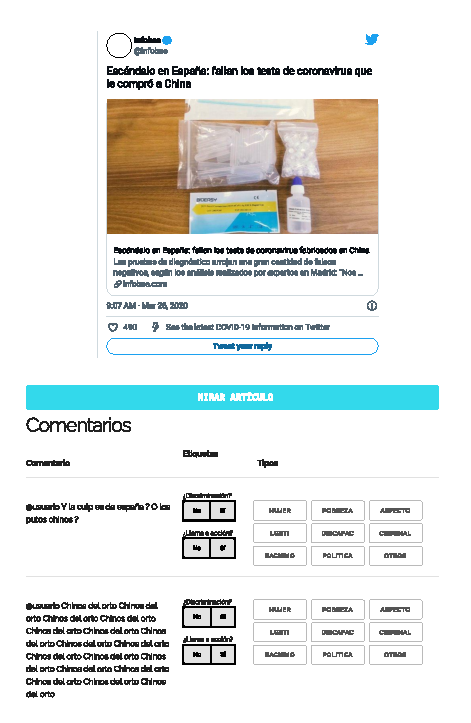
\includegraphics[width=\textwidth]{img/labeler.pdf}
    \caption{Pantalla del etiquetador}
    \label{fig:labeler_example}
\end{figure}

Al no utilizar ningún servicio de etiquetado, optamos por desarrollar nuestra propia aplicación para el etiquetado de tweets. En ella, a cada etiquetador les fueron asignados progresivamente los artículos a anotar, los cuales fueron agrupados en ``lotes'' para facilitar la tarea administrativa de la asignación.

La figura \ref{fig:labeler_example} muestra la interfaz presentada a los etiquetadores. Cada artículo es presentado al etiquetador junto a los comentarios asignados. Ante esto, el etiquetador puede elegir saltear el artículo o etiquetarlo. Si decide etiquetarlo, el etiquetador debe para cada comentario marcar usando un control de tipo ``switch''

\begin{enumerate}
    \item Si el comentario contiene discurso discriminatorio
    \item En caso de ser discriminatorio, marcar si llama a la acción
    \item En caso de ser discriminatorio, marcar al menos una característica ofendida
\end{enumerate}

Para el desarrollo de la aplicación usamos Django\footnote{\url{https://www.djangoproject.com/}}, un framework de python para desarrollo web, y Javascript plano. Como base de datos utilizamos SQLite ya que tenía una baja tasa de concurrencia (sólo 6 usuarios.)

\subsection{Esquema de anotación}

%Teniendo en cuenta el modelo de anotación ilustrado en la figura \ref{fig:annotation_model}, optamos por la siguiente metodología para el etiquetado de los comentarios de nuestro dataset.

%%
%%
%% Link a Google Draw:
%% https://docs.google.com/drawings/d/1esS9tAwpPVydohxd-B-xwVdAaPQRVGAo0MruBrgSKig/edit
%%
%%

\begin{figure}
    \centering
    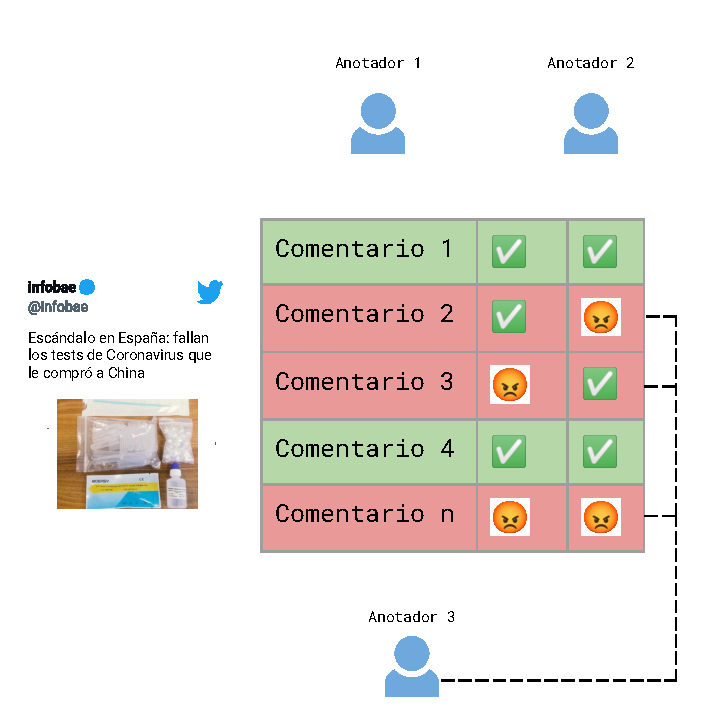
\includegraphics[width=0.75\textwidth]{img/esquema_anotacion.pdf}
    \caption{Esquema de anotación. Caso en que ambos anotadores etiqueten los comentarios del artículo}
    \label{fig:annotation_schema}
\end{figure}

Los artículos son asignados a cada etiquetador. Cada etiquetador, al serle presentado un artículo, tiene dos opciones: etiquetarlo o saltearlo. La idea de saltear era doble: evitar contenido poco ``interesante'' en términos de comentarios discriminatorios, o evitar contenido sensible para el anotador (algo que no ocurrió afortunadamente).

Una posibilidad que barajamos en un principio fue asignar para el etiquetado el artículo completo a 3 anotadores. Sin embargo, esta modalidad sería altamente ineficiente dada la baja cantidad de contenido discriminatorio. Entonces, decidimos ir por un esquema de ``desempate'': dos anotadores anotan un artículo, y luego un tercero anota sólo aquellos donde al menos uno marcó que es discriminatorio. Esto da la posibilidad de que haya una tercera anotación incluso cuando dos previas marcaron que el comentario es discriminatorio, y lo hacemos para recolectar más información. \todo{marcar otros trabajos que hayan hecho esto}. Con este esquema de anotación, y teniendo en cuenta los números finales obtenidos del dataset, dedicamos 2.16 etiquetados por comentarios versus 3 etiquetados por comentario de anotar tres veces todo. La figura \ref{fig:annotation_schema} ilustra este flujo de anotación.

Entonces, en primer lugar cada artículo es asignado a 2 anotadores. Luego de esto, se solicita una tercera anotación pero sólo sobre los comentarios que tengan alguna de las dos etiquetadas marcando contenido discriminatorio, y no dando la posibilidad de saltear. Ahora ¿qué pasa si alguno de los dos anotadores saltea el artículo?. Tenemos dos casos. Si los dos saltean el artículo, entonces descartamos ese artículo. Ahora, puede ocurrir el caso de que uno lo saltee y el otro lo anote: en ese caso, y en pos de maximizar el contenido discriminatorio encontrado o uno lo hace y el otro anota menos de 4 comentarios odiosos, entonces no pasa a 3ra anotación y lo descartamos del dataset. Si uno salteó y el otro anotador anotó 4 o más comentarios odiosos, entonces forzamos al primer anotador a anotar el artículo, sin dar esta vez opción de saltear. La figura \ref{fig:annotation_schema_case_two} ilustra el flujo para este caso.


%%
%%
%% Link a Google Draw
%% https://docs.google.com/drawings/d/1TOlCgZggCmYHgZWV7ZrIIlXuhcFUMeYw4PcFM7XdY2k/edit
%%
%%

\begin{figure}
    \centering
    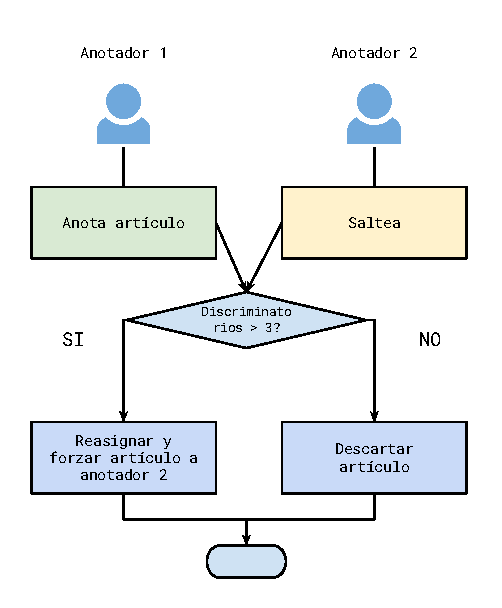
\includegraphics[width=0.75\textwidth]{img/esquema_anotacion_caso_2.pdf}
    \caption{Esquema de anotación. Caso en que ambos anotadores etiqueten los comentarios del artículo}
    \label{fig:annotation_schema_case_two}
\end{figure}


Como resultado de este esquema, cada comentario de nuestro dataset puede tener dos o tres anotaciones, siendo los casos posibles los siguientes:

\begin{enumerate}
    \item Dos anotaciones negativas
    \item Tres anotaciones, siendo al menos una que marque el comentario como discriminatorio
\end{enumerate}




\subsection{Asignación}

\citet{pustejovsky2012natural} denominan ``asignación'' al procedimiento de extraer las ``gold labels'' de las etiquetas. En este punto tenemos una etiqueta binaria si el contenido es discriminatorio o no (notamos HS) en el primer nivel, y luego 9 etiquetas binarias: una para la llamadas a la acción (CALLS) y otras 8 para las características ofendidas. Recordemos que una anotación negativa sólo consta de HS negativo, mientras que una positiva consta de un HS positivo, una etiqueta para CALLS y al menos una etiqueta positiva de las características restantes.

Para este dataset, tomamos las siguientes decisiones:

\begin{enumerate}
    \item Para la etiqueta de HS, realizamos la votación mayoritaria
    \item Si hay HS, CALLS es positivo sii es votación mayoritaria
    \item Si hay HS, marco como positivas todas aquellas características marcadas por los anotadores
\end{enumerate}

La primer decisión es la más obvia y razonable, pero las otras dos decisiones merecen alguna discusión. Para que sea un comentario considerado como HS, tiene que ocurrir que al menos dos etiquetadores lo marquen como tal. En ese caso, para que haya votación mayoritaria de CALLS, tiene que haber dos o más votos marcados como tal; en caso de empate, es decir, que un anotador marca que hay llamado a la acción y otro que no, marcamos que no hay llamado a la acción.

En el caso de las características, marcamos todas las que hayan marcado aquellos anotadores que hayan etiquetado HS. Esta decisión podría haberse tomado de otra manera; por ejemplo, sólo tomando aquellos casos donde haya cierto grado de coincidencia entre los comentarios. Sin embargo, al considerar que los límites entre las características son difusos (por ejemplo, apariencia y mujer tienen un grado de coincidencia, y a veces clasismo y racismo también) preferimos optar por este esquema.

\todo{Agregar algún gráfico de esto}

\subsection{Recursos utilizados}

El etiquetado constó de XXX horas. A cada etiquetador le fue pagado YYYY por hora, y luego ZZZ por hora en segunda instancia. Esto equivale a WWW USD.

\section{Dataset resultante}

\begin{table}
    \centering
    % \begin{tabular}{lrr}
    %     \toprule
    %     Total articles & 1238    \\
    %     Total comments &  56869  \\
    %     Hateful Tweets &   8715  \\
    %     Ratio          &   0.153 \\
    % \end{tabular}
    \begin{tabular}{lrr}
        \toprule
        Característica &  Count &  Calls to Action \\
        \midrule
        RACISM         &   2469 &              674 \\
        APPEARANCE     &   1803 &               34 \\
        CRIMINAL       &   1642 &              722 \\
        POLITICS       &   1428 &              136 \\
        WOMEN          &   1332 &               18 \\
        CLASS          &    823 &              135 \\
        LGBTI          &    818 &               11 \\
        DISABLED       &    580 &                4 \\
        \bottomrule
    \end{tabular}
    \caption{Figures of the annotated dataset, by total numbers and segmented by characteristic}
    \label{tab:dataset_figures}

\end{table}

El dataset resultante consta de 1238 artículos etiquetados, y 56869 comentarios respectivamente, de los cuales 8715 contienen contenido discriminatorio según los criterios de asignación antes referidos. Podemos observar que aproximadamente 1 de cada 6 comentarios es discriminatorio; esto no es representativo del universo de notas periodísticas ya que recordemos que la selección de los datos no fue aleatoria. La tabla \ref{tab:dataset_figures} contiene estos datos estadísticos.

De todos los tweets discriminatorios, tenemos en particular los llamados a la acción. La inmensa mayoría de estos está dirigido hacia la categoría CRIMINAL, muchos en la forma de llamados a matar a criminales y otros delincuentes.

La tabla \ref{tab:annotation_agreement} reporta el acuerdo entre anotadores usando la métrica alpha de Krippendorff \todo{agregar cita}. Reportamos el valor de $\alpha$ para HS sobre todas las etiquetas, y luego todas las etiquetas del segundo nivel del modelo jerárquico (características y llamado a la acción) sólo sobre aquellas que hayan marcado que el comentario contiene HS. Esto es equivalente a calcular el acuerdo con una etiqueta faltante en el segundo nivel para las características y el llamado a la acción. Si bien este acuerdo tiende a ser alto, debe leerse como el acuerdo sobre la razón detrás del hate speech; la mayor penalización queda reservada a HS, que tiene $\alpha = 0.59$, algo que podría marcarse como un buen acuerdo teniendo en cuenta los parámetros vistos en las tablas de preliminares. \todo{linkear esto}

\begin{table}
    \centering
    \begin{tabular}{lc}
        \toprule
        Categoría   & $\alpha$ de Krippendorff \\
        \midrule
        Hateful              &  0.579 \\
        Calls to Action      &  0.641 \\
        \midrule
        WOMEN                &  0.783 \\
        LGBTI                &  0.920 \\
        RACISM               &  0.929 \\
        CLASS                &  0.706 \\
        POLITICS             &  0.808 \\
        DISABLED             &  0.849 \\
        APPEARANCE           &  0.871 \\
        CRIMINAL             &  0.931 \\
        \bottomrule
    \end{tabular}
    \caption{Reported Agreements. \emph{Hateful} agreement is reported for the binary decision of a tweet assigned as hateful or not; for the other characteristics (and the calls to action) the agreement is calculated over those tweets with two or more hateful marks}
    \label{tab:annotation_agreement}
\end{table}




\begin{table}
    \scriptsize
    \centering
    \begin{tabular}{p{0.1\textwidth} p{0.45\textwidth} p{0.40\textwidth}}
        \hline
        Tipo & Contexto & Texto \\
        \hline
        %WOMEN & Nicole Neumann apuntó contra los consumidores de carne: “Sigan comiendo asadito” & @usuario Debieras comerte uno así te sacas esa cara agria que tenes🤣🤣👎 \\
        \mr{12}{MUJER} & Por el mundo: Florencia Peña mostró su lujosa nueva casa con bar, muelle y pileta & @usuario Cuando succionas las correctas \\
         & El exabrupto de Rodolfo Barili con una modelo que se metió en el baúl de un auto para violar la cuarentena & @usuario Barili, ojo es mujer, en cualquier momento te caen las hordas de feminazis, pero estoy al 100\% CON VOS!! \\
         & Video: tres mujeres forzaron la puerta de un edificio en Palermo y desvalijaron dos departamentos & @usuario 3 feministas , claramente es el perfil de las feministas \\
         & Británica llegó a Perú por 10 días y se quedó por amor: vive sin agua potable y entre insectos & @usuario Pero empomada todo el día... \\
         & “Me esterilicé, pero no odio a los niños”: mi vida dentro del movimiento “libre de hijos” & @usuario Es que sos incogible..quien te va a hacer un hijo.....algun ciegoooo \\
         & Mia Khalifa: actuó en videos porno durante pocos meses, cobró fama mundial y ahora lucha por borrar su pasado & @usuario JAJAJAJAAJAJAAJA SEGUILA CHUPANDO.... \\
         & ¿Se puede ser feminista y llorar a Diego Maradona? & @usuario Para las feminazis toda ilógica es correcta \\
         & Claribel Medina, indignada con un grupo de personas reunidas en un bar: “La gente está sin barbijo mientras los actores no podemos trabajar” & @usuario La menopausia nos pone locas 🤦🏽‍♀️🤣 \\
         & Narda Lepes: “Mil veces me tocaron el culo en las cocinas de los restaurantes” & @usuario Tenes lindo culo? \\
         & Un policía se defendió de un robo en Pompeya, mató a un ladrón y estuvo dos días preso & @usuario Que jueza hija de mil puta ojalá t afanen a vos y t maten un ser querido a ver qué haces LLEGUA de mierda puta \\
         & “Cristian, mirá lo que hago por vos”: quién es la modelo que se metió en el baúl de un auto para violar la cuarentena & @usuario Jajaja modelo Hot jaja Telosu!! Mami diría la Moria !! Jaja ridícula tafaldegaver \\
         & La aberrante arenga machista que dio el preparador físico de Güemes de Santiago del Estero & @usuario Que aliade te volviste Clarín, vos te culeas la que tiene olor a pingo (feminazi) \\
        \hline
        \hline
        \mr{8}{LGBTI} & Por qué Flor de la V no continuó en Mujeres de eltrece, tras la salida de Claudia Fontán & @usuario y..porque no es mujer, más claro echale agua \\
         & Histórico: Mara Gómez fue habilitada y será la primera jugadora trans en el fútbol argentino & @usuario Unos huevos bárbaros tiene esta mina!!!!! \\
         & La historia de la modelo colombiana trans que besa la panza de su esposo embarazado de ocho meses & @usuario Un macho besando a otro macho \\
         & Luis Novaresio le dedicó un romántico mensaje a Braulio Bauab por su cumpleaños & @usuario Guacale \\
         & Eugenio Zaffaroni le contestó a Sergio Berni tras la polémica por las domiciliarias: “Es el populacherismo vindicativo que llenó las cárceles” & @usuario cuando se muere este viejo trolo enfermo \\
         & La impactante historia de la tenista trans que hoy es la N° 3 de Argentina en la categoría senior femenino & @usuario Vergonzoso que  las mujeres toleren esto.\textbackslash nEse tenista debería jugar con hombres o a lo sumo, en un torneo de sujetos como él. \\
         & Joe Biden nominó a Rachel Levine, una mujer transgénero, para que sea su subsecretaria de Salud & @usuario Este presidente es la dejeneracion total del mundo \\
         & Así luce el actor Elliot Page tras declararse trans & @usuario Tiene Bija? No. Tiene Concha? Si. Es mujer entonces \\
         & El abuelo que a los 90 años confesó: “Soy gay, soy libre y estoy afuera” & @usuario Como no te agarra el Coronavirus.   🤮🤮 \\
        \hline
    \end{tabular}

    \caption{Ejemplos discriminatorios del dataset contra mujeres y la comunidad LGBTI.}
    \label{tab:women_and_lgbti_examples}
\end{table}


\begin{table}
    \scriptsize
    \centering
    \begin{tabular}{p{0.1\textwidth} p{0.45\textwidth} p{0.40\textwidth}}
        \hline
        Tipo & Contexto & Texto \\
        \hline
        \mr{9}{RACISMO} & Coronavirus: las terribles imágenes del mercado donde se originó la pandemia & @usuario Hay que matarlos hijos de puta 😑 \\
         & Malestar en Washington con el Gobierno argentino porque no dejó atracar al buque más moderno de la guardia costera de Estados Unidos & @usuario Amo ver los sudacas que se creen yankis enojados por esto. \\
         & Milagro Sala: “Seguimos presos, los que nos gobiernan tienen que cambiar las cabezas” & @usuario Negra, seguis presa por chorra. \\
         & Al menos 7 muertos en China a causa de un virus transmitido por garrapatas & @usuario Que no venga ningún chino más a la Argentina! Por favor! Ya Basta! \\
         & En China comenzó el tradicional Festival de Carne de Perro a pesar de la pandemia de coronavirus y una ONG intenta salvarlos & @usuario No soy racista, pero hay que matar a todos los chinos \\
         & Científicos identificaron en China otro virus respiratorio “con potencial para convertirse en pandemia” & @usuario Nos infectan a Todos!!! \\
         & Coronavirus. Yanzhong Huang: "Es bastante probable que ya se esté gestando un Covid-21" & @usuario Bombas urgente a esta maldita raza \\
         & Denunciaron la nueva maniobra de China para ocultar las verdaderas cifras del coronavirus & @usuario Mundialmente mantenemos china xq todo viene de ahí y hoy estamos fundidos y en emergencia... \#ChinaVirus no quiero ver un \#chino x mucho tiempo! \\
         & Villa Mascardi: impresionante operativo con tanquetas blindadas para que una fiscal ingresara a una zona controlada por mapuches & @usuario Basta!!! No son mapuches son delincuentes !!! A ver si alguien pone las pelotas donde hay que ponerlas y los cagan a tiros de una vez !!! \\
        \hline
        \hline
        %\rotatebox[origin=c]{90}{rota}
        \mr{5}{CRIMINAL} & Aberrante: un político de Misiones admitió haber esclavizado y violado a sus tres hijastras & @usuario Solo se requiere una bala. \\
         & Rosario: un grupo de vecinos linchó y mató a golpes a un joven acusado de robar autos & @usuario esta perfecto, ejemplo a los demás \\
         & El panadero que mató a un ladrón en La Matanza: "No soy un asesino, estoy arrepentido" & @usuario Que dice señor ! No sé arrepienta, que hizo una obra de bien.Era su vida o la del delincuente. \\
         & Video: salió de la cárcel por el coronavirus y murió de un tiro el mismo día al festejar su libertad & @usuario Justicia divina!! \\
         & Le sacó el arma al ladrón que lo asaltó, lo corrió y lo mató de un disparo: quedó detenido & @usuario Buenísimo vamos por el exterminio total de estos primates. \\
        \hline
        \hline
        \mr{8}{CLASE} & La Justicia ordenó el desalojo de la masiva toma de terrenos en Guernica & @usuario Lanzallamas y a otra cosa \\
         & Hubo tensión en la Quinta de Olivos entre un grupo que apoyaba a Alberto Fernández y manifestantes del banderazo contra el Gobierno & @usuario PLANEROS Y BARRABRAVAS \\
         & Organizaciones sociales cortaron la avenida 9 de Julio: reclamaron un salario mínimo de \$ 45.000 & @usuario Vayan a lo laburar hdp. \\
         & La historia de una familia de cartoneros en la toma de Guernica: “Por primera vez sentimos que tenemos un hogar” & @usuario Bala. \\
         & El Gobierno autorizó la apertura de las escuelas porteñas para las elecciones de Bolivia & @usuario No sería mejor deportar a los bolivianos indocumentados?.además nos suman pobreza e indigencia \\
         & Coronavirus en Argentina: un dirigente radical deseó que la pandemia “haga una limpieza étnica” con “negros de La Matanza” & @usuario Es el deseo de todo argentino de bien \\
         & El Polo Obrero realiza un corte en la Panamericana en contra de la flexibilización de la cuarentena y en reclamo de aumentos a los planes sociales & @usuario Clarísimo que no quieren laburar y quieren vivir de nosotros! \\
         & Coronavirus en la Argentina: movimientos sociales reclaman asistencia alimentaria en el Obelisco & @usuario Anda a laburar lpqtp \\
        \hline
    \end{tabular}

    \caption{Ejemplos discriminatorios del dataset por motivos de clase, racismo, o contra criminales.}
    \label{tab:class_racism_examples}
\end{table}


\begin{table}
    \scriptsize
    \centering
    \begin{tabular}{p{0.1\textwidth} p{0.45\textwidth} p{0.40\textwidth}}
        \hline
        Tipo & Contexto & Texto \\
        \hline

     \mr{5}{POLITICA} & Confirman una mutación en el coronavirus que puede hacerlo 10 veces más contagioso que la cepa original de Wuhan & @usuario ME ALEGRO MUCHÍSIMO.\textbackslash nOJALÁ LLEGUE PRONTO A ARGENTINA Y ARRASE CON TODO.\textbackslash nPODRÍAMOS VER AL FIN ALGO MÁS DAÑINO QUE EL CÁNCER PERONISTA Y SU METÁSTASIS KIRCHNERISTA. \\
      & Murió un nieto recuperado por Abuelas de Plaza de Mayo: los mensajes de Alberto Fernández y Cristina Kirchner & @usuario Un planero menos. \\
      & Última encuesta: ¿Qué mujer superó a Alberto Fernández en imagen positiva? & @usuario Les ahorro el clickbait. Es Vidal, igual perdió por 20 puntos. Gorila LTA. \\
      & Cómo es la cerveza “peronista” que el Chacho Coudet le regaló a Alberto Fernández & @usuario Debe ser meo de gato. berreta como todo lo peroncho \\
      & El descargo de Nicolás Wiñazki después de que Vero Lozano se burlara de él: “Quizás le afecta la cuarentena” & @usuario Yo creo que al revés, patético operador. Solo los gorilas pueden bancarte croto \\
      \hline
      \hline
    \mr{5}{APARIENC.} & Axel Kicillof recomendó una “cuarentena previa” de 14 días para “llegar sanos a Navidad y Año Nuevo” & @usuario Chuoame la verga enano moishe \\
     & Video indignante: piba violó la cuarentena y viajó en el baúl de un taxi para ver a un chico & @usuario Habría qur buscar también y meter en cana al cirujano que le hizo la nariz!! Parece Michael Jackson la loca!!! \\
     & El senador José Mayans defendió a Gildo Insfrán: “En pandemia no hay derechos” & @usuario Volve al gancho , docer \\
     & El video sexy de More Rial en corpiño & @usuario Asco \\
     & El sensual paseo en moto de Florencia Peña: "Próxima parada: tu casa" & @usuario Que tiene de sensual, ésta vieja cascoteada?prostituta de cuarta,kukaracha inmunda! \\

    \hline
    \hline
    \mr{4}{DISCAPAC.}& Patricia Bullrich pidió ser drásticos con los docentes: “El que no va, tendrá que ser reemplazado” & @usuario Estragos del tinto \\
      & El abuelo que a los 90 años confesó: “Soy gay, soy libre y estoy afuera” & @usuario Alhzeimer o demencia senil!!!!! \\
      & Elisa Carrió dijo que “ninguna pandemia es excusa para suspender la República” y advirtió que “vienen por los campos” & @usuario Si sacan a la paciente psquiatrica es porque están hasta las manos.\textbackslash n\#CarcelACambiemos \\
      & Florencia Kirchner y su posteo a favor de la amistad: "Nunca entendí la desesperación por la pareja" & @usuario La enfermita está mejor que yo,y no se calienta por la hija \\
    \hline
    \mr{6}{INCITACIÓN} & Harán un listado de los presos en situación de riesgo por el coronavirus para evaluar si deben salir de prisión & @usuario @usuario Todo al reves! Si hay alguno con coronavirus PONGANLO EN EL MEDIO! \\
         & La advertencia de Juan Grabois: “Van a haber 1, 5, 20 Guernicas” & @usuario @usuario Habra 100 paredones \\
         & Otro caso de peste bubónica enciende las alarmas en China & @usuario Una atómica a China... \\
         & Coronavirus: afirman que volvió la venta de carne de murciélagos en China & @usuario Boicot a todo producto chino!!! \\
         & Villa Mascardi: impresionante operativo con tanquetas blindadas para que una fiscal ingresara a una zona controlada por mapuches & @usuario El Diálogo se Inicia con BALAS y Finaliza con La Última \\
         & Coronavirus en China: la ciudad de Shenzhen prohíbe comer perros y gatos & @usuario habrá alguna manera de erradicar a estos tipos del mundo ? \\
    \hline
    \hline
    \end{tabular}
    \caption{Ejemplos discriminatorios del dataset. INCITACIÓN refiere a los llamados a realizar algún tipo de medida contra el grupo o la persona atacada. }
    \label{tab:politics_and_calls_examples}
\end{table}



\subsection{Anonimización para publicación de los datos}



\section{Conclusión}

En este capítulo, describimos la construcción de un dataset contextualizado de lenguaje discriminatorio o hate speech. Para ello, recolectamos respuestas a noticias periodísticas posteadas en Twitter por los principales medios de noticias de Argentina. Exploramos distintas alternativas para la selección de artículos a etiquetar, tanto observando los tópicos de los artículos como los comentarios a este. Decidimos elegir los artículos en base a sus comentarios potencialmente discriminatorios, y luego seleccionar una muestra aleatoria y acotada de comentarios.

Para realizar la tarea de etiquetado, desarrollamos nuestra propia herramienta la cual hacemos pública. Definimos un modelo de anotación jerárquico y granular para la tarea, siendo relativamente novedoso el hecho de anotar las características ofendidas en cada texto social. Seis etiquetadores nativos de la variedad dialectal rioplatense realizaron la tarea de anotación bajo un esquema de 2 anotaciones + desempate.

Como producto, obtuvimos un dataset de cerca de 57k comentarios repartidos en 1.2k artículos, una cantidad de tamaño considerable aunque no tengamos parámetro de comparación ya que no existen muchos datasets similares. De los 57k comentarios, alrededor de 8k comentarios tienen contenido discriminatorio (una tasa de 1 cada 6). Un análisis exploratorio de los comentarios discriminatorios muestra ejemplos complejos y ricos, algunos de ellos altamente dependientes del contexto.

En el siguiente capítulo, abordaremos nuestra pregunta original: ¿puede el contexto ayudar a los algoritmos de clasificación a mejorar su performance?. Para responder esto, utilizaremos este dataset especialmente diseñado.


\chapter{Clasificadores, Análisis y Limitaciones}

En este capítulo abordaremos una de las preguntas centrales de la tesis: ¿puede ayudar el contexto a mejorar la performance de métodos automáticos de lenguaje de odio? Para intentar contestar esta pregunta, utilizaremos el dataset que construímos en el capítulo \ref{chap:dataset_creation}, y aplicaremos técnicas del estado del arte basadas en transformers. Exploraremos dos versiones de clasificadores: descontextualizadas, donde sólo observamos el comentario analizado; y contextualizadas, donde podemos consumir el título o el título y el cuerpo del artículo.

Proponemos en este capítulo dos tareas: detección ``plana'', donde sólo predecimos la característica de si hay o no discurso de odio; y la detección ``granular'', donde además predecimos todas las características ofendidas (potencialmente más de una). Analizaremos el impacto de agregar contexto para cada una de estos problemas de clasificación.


\section{Trabajos previos}

Como contamos en la anterior sección, son pocos los trabajos y datasets que poseen contexto. Ver \ref{sec:dataset_previous} para un repaso de los distintos datasets contextualizados.

\citet{gao-huang-2017-detecting} propone dos tipos de modelos: regresiones logísticas y redes neuronales recurrentes. Para los modelos de regresiones logísticas, usan como inputs bolsas de palabras, bolsas de caracteres, vectores semánticos producidos con Linguistic Inquiry and Word Count (LIWC) \cite{pennebaker2001linguistic} y features de un lexicon de emociones \cite{mohammad2013nrc}. Por otro lado, utiliza LSTM bidireccionales con mecanismo de atención de Bahdanau \cite{bahdanau2014neural} usando embeddings \emph{word2Vec} de dimensión 100.

Un punto criticable de este trabajo es que utiliza el nombre de usuario como feature; algo que a priori no suele hacerse ya que permitiría ``prejuzgar'' a un usuario antes que por el contenido de sus tweets. Si bien es cierto que la información de usuarios y sus conexiones es valiosa, introducir esta información a nuestros modelos da lugar a posibles correlaciones espurias que es preferible evitar.


\begin{figure*}[t]
    \centering
    \begin{minipage}[b]{0.49\textwidth}
        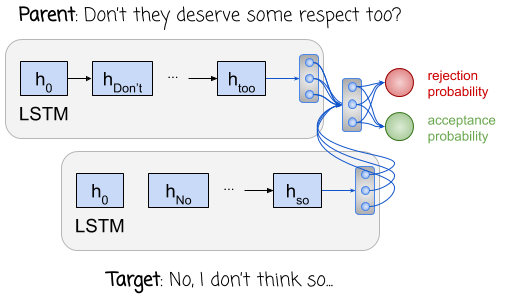
\includegraphics[width=\textwidth]{img/pavlopoulos_rnn_rnn_classifier.png}
    \end{minipage}
    \hfill
    \begin{minipage}[b]{0.49\textwidth}
        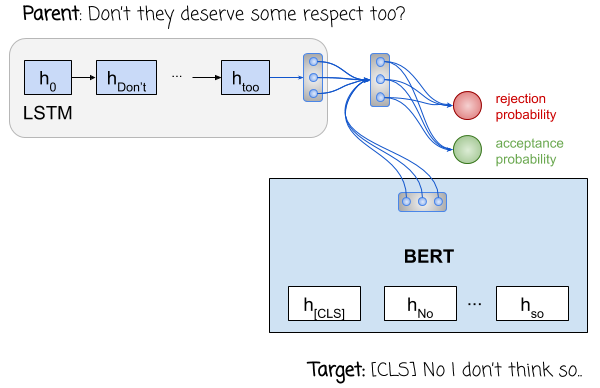
\includegraphics[width=\textwidth]{img/pavlopoulos_rnn_bert_classifier.png}
    \end{minipage}

    \begin{minipage}[b]{0.35\textwidth}
        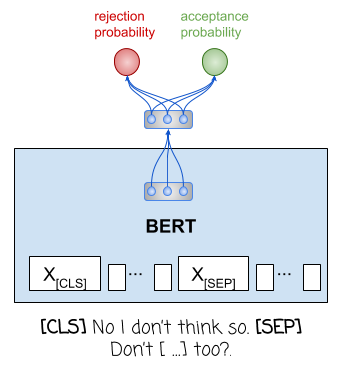
\includegraphics[width=\textwidth]{img/pavlopoulos_bert_sep_classifier.png}
    \end{minipage}


    \caption{Clasificadores que consumen contexto propuestos por \citet{pavlopoulos2020toxicity}. Los dos primeros clasificadores proponen una arquitectura de dos encoders, uno para el texto y otro para el contexto usando bi-LSTMs y BERT como posibilidades. El tercer clasificador propuesto es un BERT usando su estructura natural para codificar dos oraciones separadas por el token $SEP$ }
    \label{fig:pavlopoulos_classifiers}
\end{figure*}


En la sección \ref{sec:dataset_previous} hemos descripto el dataset construído por \citet{pavlopoulos2020toxicity}. Nos detendremos un momento para analizar sus experimentos de clasificación  ya que guardan importantes similaridades con lo que haremos en este capítulo. En ese trabajo se obtuvieron dos datasets de entrenamiento, uno etiquetado viendo el contexto y otro sin verlo. El dataset de test fue etiquetado viendo el contexto, considerando que el etiquetado es de mejor calidad usando más información. Tenemos entonces, dos preguntas: ¿mejora la performance de la tarea usando el dataset etiquetado con contexto? ¿mejora la performance del clasificador consumiendo información contextual? Estas dos preguntas nos brinda entonces dos elecciones: dataset de entrenamiento con o sin contexto, y clasificador con o sin contexto. Tenemos 4 posibles combinaciones de experimentos, sin aún considerar posibles técnicas de clasificación.

Para cada una de estas combinaciones, se consideraron técnicas del estado del arte de clasificación. Para aquellos clasificadores que no consumen contexto, las opciones son las mismas que hemos visto en capítulos anteriores: bi-LSTM o BERT. Para aquellos que sí consumen contexto, se evaluan dos estrategias: una, concatenar con algún caracter, y otra usando dos encoders distintos para el contexto y el texto. A su vez también utilizan la API Perspective de Google \todo{Agregar alguna cita de esto, y quizás alguna explicación en capítulo 4}.

Para todas las combinaciones posibles, si bien hay una mejora en la performance medida con ROC-AUC al usar contexto en ambas formas, esta no es significativa. De esto los autores concluyen que no pueden encontrar evidencia suficiente sobre la utilidad del contexto en la detección de toxicidad.

Algo a mencionar (que retomaremos en este y en el siguiente capítulo) es que usan dos versiones de BERT: una usando los pesos del modelo de BERT, y otro haciendo un ajuste de dominio () corriendo la tarea de MLM sobre un dataset grande y no etiquetado. En el caso de el trabajo mencionado, sólo hacen un fine-tuning sobre comentarios sueltos del dataset de Civil Comments. Esto podría tener algún efecto deteriorando la performance al usar contexto; sin embargo, en el BERT a secas (sin hacer ajustes) tampoco se observa mejora significativa en la performance.

Algunas limitaciones marcadas por los autores son:

\begin{itemize}
    \item Contexto muy pequeño: sólo el título más el comentario previo
    \item Se ignora el hilo completo de comentarios
    \item Los datos fueron sampleados aleatoriamente
\end{itemize}

En \citet{xenos-2021-context}, continuación de este trabajo, reetiquetaron el dataset de Civil Comments usando contexto y --como mencionamos en la sección \ref{sec:dataset_previous}-- presentaron una nueva tarea de detección de sensibilidad al contexto. Usando la API Perspective (y la estrategia de concatenación ``básica'' con algún caracter), notaron que la performance del clasificador que consume el contexto mejora con respecto al que no lo hace a medida que restringimos nuestra atención a comentarios más ``sensibles al contexto'' (de acuerdo a la métrica definida por los autores)


\section{Tareas de clasificación propuestas}



Ahora que tenemos este corpus especialmente diseñado que contiene el contexto, ahora dirigimos nuestra atención a responder nuestra pregunta original: ¿pueden los clasificadores aprovechar el contexto para mejorar su desempeño en la tarea de detección del discurso discriminatorio? Para ello, proponemos las siguientes tareas de clasificación:

\begin{enumerate}
    \item \textbf{Detección ``plain''}: Dado un tweet y su contexto, predecir si contiene contenido discriminatorio
    \item \textbf{Detección ``fine-grained''}: Dado un tweet y su contexto, predecir las características ofendidas (si hay alguna) y si contiene un llamado a la acción
\end{enumerate}


Puede pensarse la tarea de detección plana (la que usualmente se aborda en la literatura sobre el tema) como una relajación de la tarea detallada: mientras la primera sólo nos permite detectar si hay o no contenido discriminatorio, la segunda nos pide información más precisa acerca de las características ofendidas. Estas segunda tarea es posible dado que el dataset que construímos contiene esta información, algo usualmente faltante en otros datasets.

La tarea en su versión fine-grained nos permite a su vez tener mayor entendimiento de la salida e interpretar mejor sus errores, principalmente los falsos positivos. La figura \ref{fig:hate_detection_tasks} ilustra las dos tareas propuestas. Mientras en la tarea plana sólo debemos decidir la frontera entre si el contenido es discriminatorio o no, en la tarea fine-grained necesitamos decir en cuál de todas las intersecciones está el comentario y su contexto.

Planteándolos como problemas de clasificación, la detección plana consta de predecir una sola etiqueta binaria, mientras que la tarea fine-grained consta de $n$ etiquetas binarias; es decir, $n$ problemas distintos de clasificación. Vale mencionar que, entendiendo una tarea como una relajación de la otra, si tenemos un clasificador entrenado para la tarea fine-grained podemos construir un clasificador para la tarea plana tomando la disyunción lógica de sus salidas. Retomaremos esta idea más adelante al hablar de cómo evaluamos nuestras técnicas de clasificación para cada tarea.

\begin{figure}[t]
    \centering
    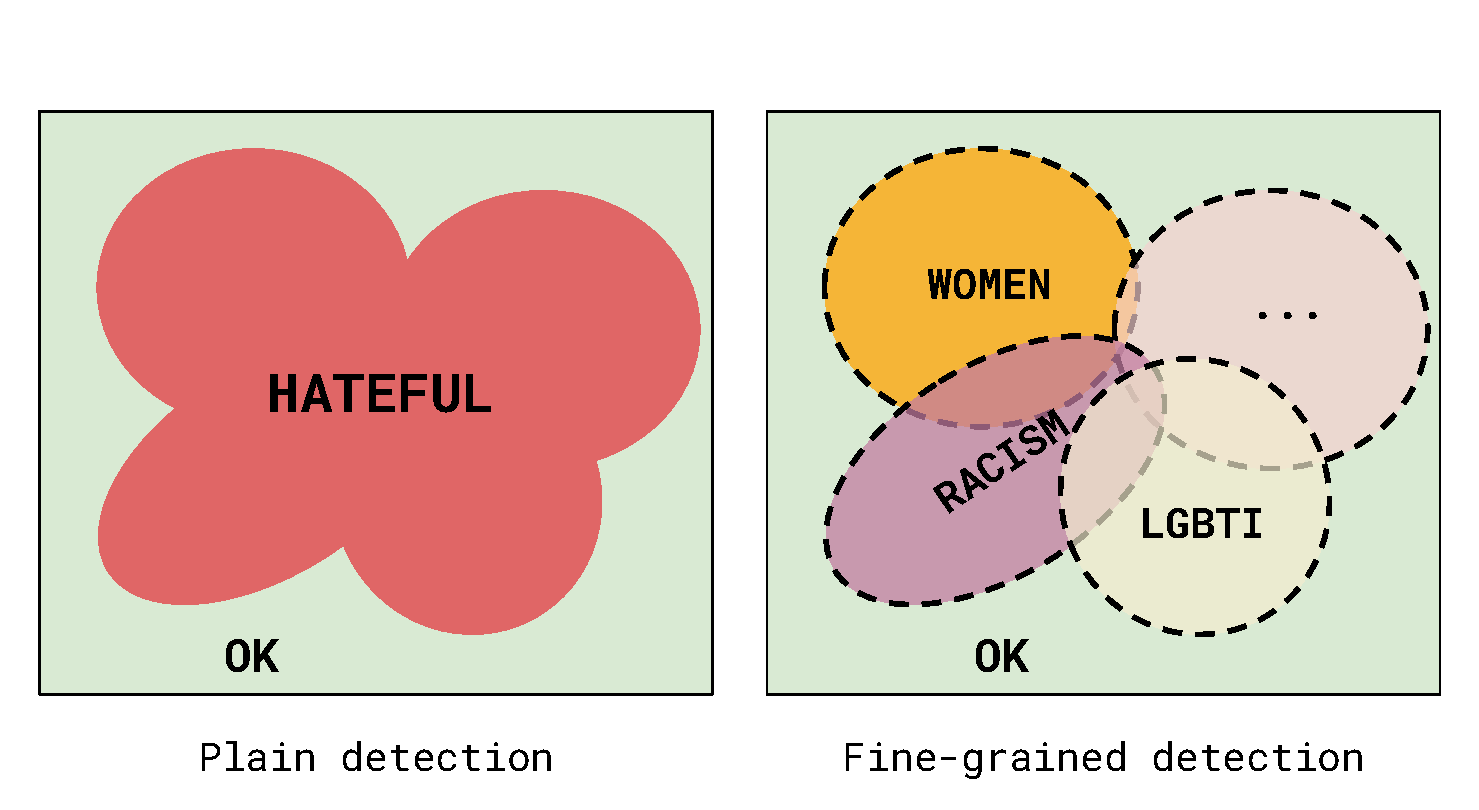
\includegraphics[width=\textwidth]{img/hate_detection_tasks.pdf}
    \caption{Tareas propuestas de detección}
    \label{fig:hate_detection_tasks}
\end{figure}

To test our hypothesis, for each task we trained classifiers having as input the following comibinations:

\begin{enumerate}
    \item The comment
    \item The title and the comment
    \item The title, the body and the comment
\end{enumerate}


\subsection{Cotas a la performance}

\begin{table}
    \centering
    \begin{tabular}{lll|ll}
        \hline
                   & \multicolumn{2}{c}{Entre anotadores} & \multicolumn{2}{c}{Contra gold} \\
        {}         &  F1 mean&  F1 median  & F1 Mean  &  F1 Median \\
        \hline
        HATEFUL    &  0.6525 &   0.6751    & 0.8285   &   0.8515   \\
        CALLS      &  0.6042 &   0.7037    & 0.7741   &   0.9148   \\
        WOMEN      &  0.7258 &   0.7368    & 0.8371   &   0.8275   \\
        LGBTI      &  0.8939 &   0.9600    & 0.9660   &   0.9743   \\
        RACISM     &  0.9458 &   0.9592    & 0.9667   &   0.9731   \\
        CLASS      &  0.7310 &   0.7500    & 0.8058   &   0.8391   \\
        POLITICS   &  0.7370 &   0.7777    & 0.8920   &   0.9189   \\
        DISABLED   &  0.7973 &   0.8800    & 0.8976   &   0.9392   \\
        APPEARANCE &  0.8033 &   0.9024    & 0.9026   &   0.9493   \\
        CRIMINAL   &  0.8180 &   0.9473    & 0.9614   &   0.9788   \\
        \hline
    \end{tabular}
    \caption{Estadísticos de los cálculos de F1 entre anotadores - modo jerárquico}
    \label{tab:ia_f1_scores}
\end{table}

Como observamos en la anterior sección, la tarea de detección de lenguaje discriminatorio contiene una alta cantidad de ruido, y el acuerdo entre humanos es moderado. En este contexto, cabe preguntarse cuál es la máxima performance que puede lograr un clasificador para esta tarea. Por la misma naturaleza del problema, claramente no puede ser perfecta.

Para obtener algunas medidas de esto, calculamos en primer lugar las F1 usando todos los posibles pares de anotadores. Como la F1 es simétrica (invirtiendo roles se invierten la precisión y la sensibilidad) no necesitamos hacer ninguna asunción sobre cuál sus roles.

Algo a tener en cuenta es que nuestra métrica final será contra la etiqueta resultante del (nuestro \emph{gold standard}). Una cota que seguro está por arriba de nuestra performance es el acuerdo que haya entre los anotadores y este \emph{gold standard}; hay que también observar que cada etiqueta ``de oro'' codifica información de sus anotaciones, con lo cual éste número es una cota superior sin dudas pero también pueden ser demasiado ``gruesa''.

La tabla \ref{tab:ia_f1_scores} contiene estadísticos de estos cálculos, tanto entre anotadores como contra el \emph{gold-standard}. Como podemos observar, la mediana entre anotadores de la F1 (usada para obviar outliers) es relativamente baja para la detección de odio ($\sim 0.67$), mientras que contra el gold standard es de $0.85$. De esto entendemos que la performance máxima en la detección está entre esos dos números.

Por otro lado, para el resto de las características observamos números más elevados, pero hay que recordar que estos cálculos están hecho \textbf{solamente} entre tweets etiquetados como odiosos. Si obviamos esta restricción (lo que llamamos ``modo libre''), la performance esperada baja sustancialmente. La tabla \ref{tab:ia_f1_scores_free_mode} muestra estos números, tanto calculado entre anotadores como contra el \emph{gold standard}.

\begin{table}
    \centering
    \begin{tabular}{lll|ll}
        \hline
                   & \multicolumn{2}{c}{Entre anotadores} & \multicolumn{2}{c}{Contra gold} \\
        {}         &  F1 mean&  F1 median  & F1 Mean  &  F1 Median \\
        \hline
        CALLS      &  0.4341 &   0.4950   &  0.7042   &   0.8424  \\
        WOMEN      &  0.4896 &   0.4676   &  0.7406   &   0.7593  \\
        LGBTI      &  0.5959 &   0.5765   &  0.8462   &   0.9152  \\
        RACISM     &  0.6532 &   0.6444   &  0.8712   &   0.8789  \\
        CLASS      &  0.4431 &   0.4444   &  0.7220   &   0.7317  \\
        POLITICS   &  0.4609 &   0.4360   &  0.7951   &   0.8155  \\
        DISABLED   &  0.5502 &   0.6000   &  0.8127   &   0.8421  \\
        APPEARANCE &  0.6485 &   0.7428   &  0.8314   &   0.9146  \\
        CRIMINAL   &  0.5265 &   0.5801   &  0.8415   &   0.9292  \\
        \bottomrule
    \end{tabular}

    \caption{Estadísticos de los cálculos de F1 entre anotadores - modo libre. Cada característica es tomada como una etiqueta binaria independientemente del cálculo de odio}
    \label{tab:ia_f1_scores_free_mode}
\end{table}


\subsection{Preprocessing}

Para cada tweet, aplicamos el siguiente procesamiento previo: primero, cortamos las repeticiones de caracteres hasta tres ocurrencias; risas normalizadas; los identificadores de usuario (\emph{@user}) se reemplazan por un token especial \emph{[USER]}; convertimos emojis en una representación de texto usando la biblioteca de python \emph{emoji} \footnote {\url{https://github.com/carpedm20/emoji/}}. Los hashtags se eliminan, están rodeados por una ficha especial \emph{[HASHTAG]} y se dividen en palabras si están en mayúsculas.

Aunque no realizamos un análisis de ablación para evaluar el impacto de cada paso del preprocesamiento, el proceso general pareció mejorar el rendimiento de la clasificación en el conjunto de datos de desarrollo.

\subsection{Clasificadores}


%%
%%
%% Link a Draw
%% https://docs.google.com/drawings/d/1F8iVSIRqHhGkQ0zglxqXLGD36RHZ9OhHMZYsg_xFOS4/edit
%%
%%

\begin{figure}
    \centering
    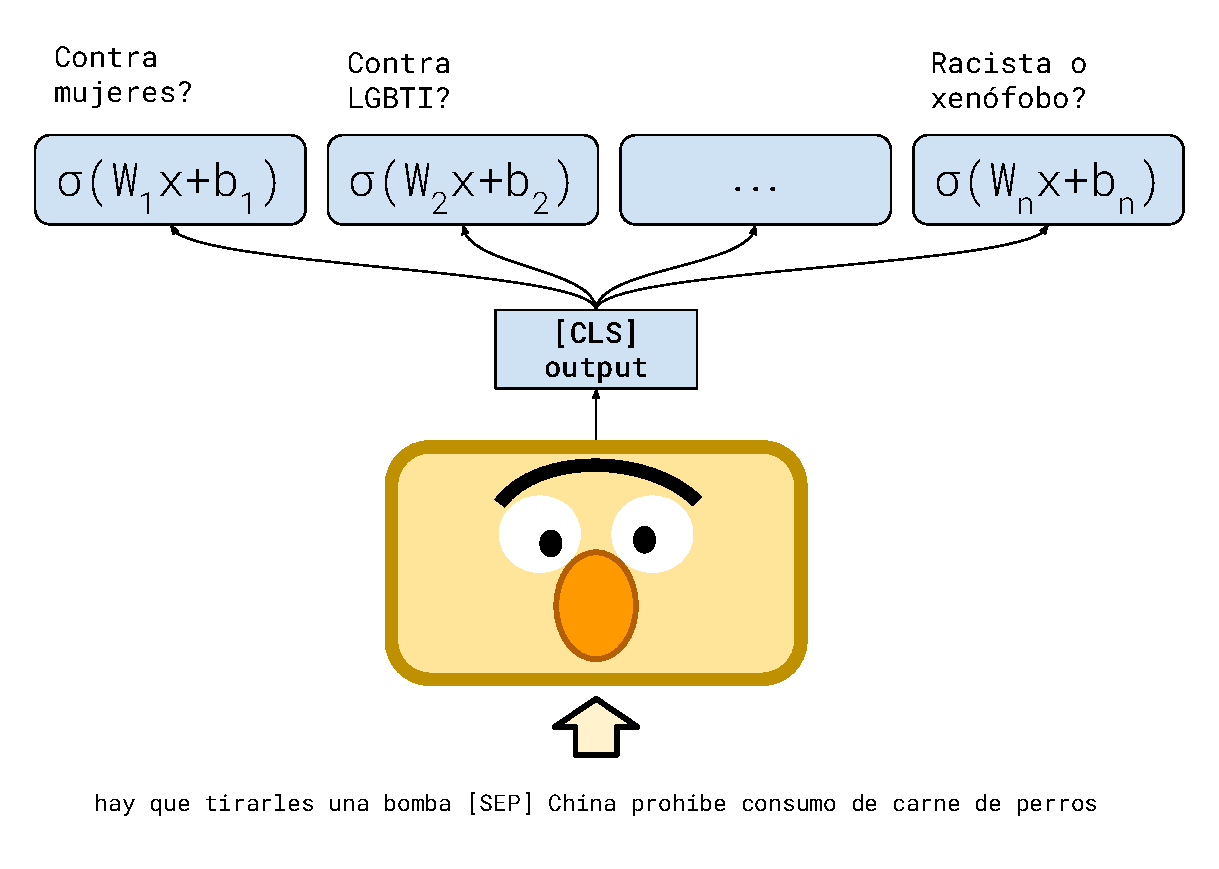
\includegraphics[width=\textwidth]{img/bert_multioutput.pdf}
    \caption{Muestra de la recolección de datos}
    \label{fig:bert_classifier}
\end{figure}


Los clasificadores propuestos se basan en \emph{BETO}\cite{canete2020spanish}, una versión en español de \emph{BERT} \cite{devlin2018bert}. \emph{BETO} tiene un tamaño similar a \emph {BERT Base}, y tiene 12 capas de transformadores con 12 cabezas de atención cada una, sumando 110 millones de parámetros. Para obtener más referencias sobre arquitecturas BERT y Transformer, sugerimos CITA NECESARIA.

Para la tarea de detección del discurso de odio, presentamos versiones sin contexto y conscientes del contexto, utilizando el título y el cuerpo completo como posibles contextos. Usamos el token especial BERT \emph {[SEP]} para codificar el contexto y el texto analizado. Recuerde que el token \emph {[SEP]} se usa para la tarea de predicción de la siguiente oración (tarea NSP) en el preentrenamiento al estilo BERT.

En cuanto a la detección de características ofendidas, consideramos este problema como una tarea de clasificación multibinaria; es decir, dado un texto odioso y una característica protegida, lo consideramos como una tarea de clasificación binaria para predecir si el texto ofende la característica respectiva. En lugar de entrenar un clasificador diferente para cada característica, entrenamos un BERT de múltiples salidas, compartiendo todos sus pesos con la excepción de 9 capas lineales diferentes para cada salida. La pérdida utilizada es

\begin{equation*}
    J = \sum\limits_{c \in CHAR \cup \{CALLS\}} J_c
\end{equation*}

donde $CHAR$ es el conjunto de todas las características protegidas (MUJERES, LGBTI, RACISMO, CLASE, etc.) y $CALLS$ es `` llamadas a la acción ''. $ J_c $, ya que cualquier $ c $ es una pérdida de entropía cruzada binaria.

Para tener costos computacionales más amigables, limitamos nuestras secuencias a 128, 256 y 512 tokens para el modelo no contextualizado, el modelo de título y el modelo de título y cuerpo, respectivamente.


\section{Resultados}


\begin{table*}[ht!]
    \centering
    \begin{tabular}{lllll}
        \toprule
        Model &          Precision &             Recall &                 F1 &           Macro F1 \\
        \midrule
        BERT No Context &  $0.682 \pm 0.020$ &  $0.593 \pm 0.018$ &  $0.634 \pm 0.006$ &  $0.785 \pm 0.003$ \\
        BERT Title      &  $0.751 \pm 0.012$ &  $0.603 \pm 0.011$ &  $0.669 \pm 0.007$ &  $0.807 \pm 0.004$ \\
        BERT Title+Body &  $0.738 \pm 0.008$ &  $0.616 \pm 0.005$ &  $0.671 \pm 0.004$ &  $0.808 \pm 0.002$ \\
        \bottomrule
    \end{tabular}


    \caption{Task A: Hate speech detection classification results. Each row contains the performance of the models in complexity order: from the model having no context to the model having full context (title and body). }
    \label{tab:task_a_results}
\end{table*}


La tabla \ref{tab:task_a_results} contiene los resultados de la clasificación, medidos por precisión, recuperación, F1 y Macro F1 (como se acostumbra en algunas tomas compartidas de Detección de discurso de odio y lenguaje ofensivo). Podemos observar que agregar contextos parece mejorar el desempeño; en particular, el simple hecho de agregar el título parece proporcionar suficiente contexto para la tarea de detección del discurso de odio. Agregar el cuerpo mejora marginalmente el rendimiento, pero a un costo computacional más alto (recuerde que la longitud máxima con título se establece en 256, y en el otro caso es 512). La mejora en la puntuación de F1 con solo agregar el título es de aproximadamente 3 puntos; título y cuerpo suma alrededor de 3,5 puntos F1 sobre la clasificación no contextualizada. Al analizar los modelos contextuales, el cuerpo completo parece mejorar el recuerdo al tiempo que disminuye ligeramente la precisión, con una puntuación general igual de F1 que el modelo de solo título.

\begin{figure*}[t]
    \centering
    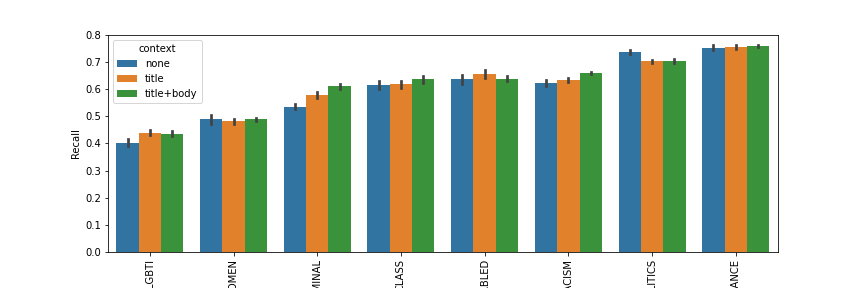
\includegraphics[width=\textwidth]{img/recall_category.png}
    \caption{Recall by characteristic for each model}
    \label{fig:recall_by_characteristic}
\end{figure*}

La figura \ref{fig:recall_by_characteristic} muestra la recuperación de nuestros algoritmos. Usar solo el contexto del título mejora la sensibilidad para las características LGBTI y CRIMINALES (Mann Whitney U, $ p \ leq 0.01 $, Bonferroni corregido); agregar el cuerpo completo también lo mejora significativamente para la característica RACISMO y lo mejora un poco más para CRIMINAL (Mann Whitney U $ p \ leq 0.01 $, Bonferroni corregido). Sin embargo, el desempeño en POLÍTICA empeora al agregar contexto en cualquier forma ($ p \ leq 0.001 $, corregido Bonferroni). Para las otras características, el contexto no mejora ni empeora el desempeño.


% \begin{table}
%     \centering
%     \begin{tabular}{ll}
%         \toprule
%         Model &            Mean F1 \\
%         \midrule
%         BERT No Context &  $0.731 \pm 0.004$ \\
%         BERT Title      &  $0.808 \pm 0.006$ \\
%         BERT Title+Body &  $0.824 \pm 0.006$ \\
%         \bottomrule
%     \end{tabular}
%     \caption{Mean F1 scores for Task B: Offended characteristic detection}
%     \label{tab:task_b_results}
% \end{table}

La figura \ref{fig:task_b_results} muestra los resultados de la característica ofendida y la tarea de detección de llamada a la acción. La tabla \ref{tab:task_b_results} muestra las puntuaciones F1 medias para tener una medida de resumen. Como se esperaba, la ganancia de tener contexto disponible es más evidente en este punto, con una diferencia media de puntuación F1 de $ 7,6 $ puntos entre no tener contexto y tener el título, y $ 1,5 $ puntos adicionales si el cuerpo está disponible. La detección de llamadas a la acción apenas se mejora al tener un contexto disponible. Nuevamente, las características LGBTI y CRIMINALES se benefician enormemente del contexto; La característica CLASS también parece tener alguna mejora. No hay grandes diferencias entre tener el título y el cuerpo completo.

\begin{figure*}[t]
    \centering
    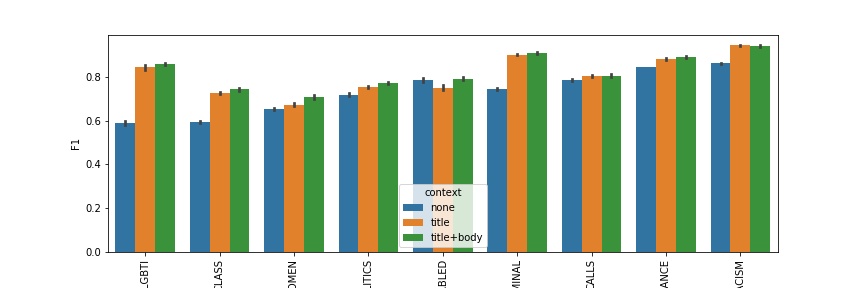
\includegraphics[width=\textwidth]{img/task_b_scores.png}
    \caption{F1 scores for each characteristic in Task B: offended characteristic detection}
    \label{fig:task_b_results}
\end{figure*}

\begin{table*}
    \centering
    \begin{tabular}{llll}
        \toprule
        {} &    BERT No Context &         BERT Title &    BERT Title+Body \\
        \midrule
        Calls F1       &  $0.784 \pm 0.009$ &  $0.802 \pm 0.010$ &  $0.805 \pm 0.017$ \\
        Women F1       &  $0.652 \pm 0.011$ &  $0.672 \pm 0.015$ &  $0.708 \pm 0.017$ \\
        Lgbti F1       &  $0.590 \pm 0.018$ &  $0.843 \pm 0.021$ &  $0.857 \pm 0.012$ \\
        Racism F1      &  $0.863 \pm 0.005$ &  $0.943 \pm 0.004$ &  $0.939 \pm 0.007$ \\
        Class F1       &  $0.593 \pm 0.011$ &  $0.727 \pm 0.012$ &  $0.742 \pm 0.014$ \\
        Politics F1    &  $0.718 \pm 0.015$ &  $0.753 \pm 0.007$ &  $0.771 \pm 0.012$ \\
        Disabled F1    &  $0.786 \pm 0.016$ &  $0.750 \pm 0.029$ &  $0.791 \pm 0.015$ \\
        Appearance F1  &  $0.845 \pm 0.004$ &  $0.879 \pm 0.010$ &  $0.892 \pm 0.010$ \\
        Criminal F1    &  $0.744 \pm 0.009$ &  $0.901 \pm 0.008$ &  $0.907 \pm 0.008$ \\
        \hline
        Mean F1        &  $0.731 \pm 0.004$ &  $0.808 \pm 0.006$ &  $0.824 \pm 0.006$ \\
        Mean Precision &  $0.786 \pm 0.004$ &  $0.853 \pm 0.007$ &  $0.851 \pm 0.006$ \\
        Mean Recall    &  $0.687 \pm 0.006$ &  $0.770 \pm 0.008$ &  $0.800 \pm 0.007$ \\
        \bottomrule
    \end{tabular}
    \caption{Performance of models for Task B: offended characteristic detection. Mean and standard deviation for 15 runs are displayed. }
    \label{tab:task_b_results}
\end{table*}


\section{Análisis de error}

\section{Discusión}

Para esta tarea en particular, podemos observar que el contexto parece dar una mejora moderada en la tarea de detección del discurso de odio (alrededor de 3 puntos F1), ninguna mejora significativa en la detección de llamadas a la acción, y una mejora considerable en la tarea característica ofendida (alrededor de 7 puntos F1 medios).

Si bien este resultado podría estar en aparente contradicción con un trabajo reciente que no encontró ninguna mejora mediante el contexto en la detección de toxicidad \cite{pavlopoulos2020toxicity}, se puede señalar que la detección del discurso de odio es una de las formas más complejas de ``tóxico'' comportamiento y, como tal, podría permitir que los clasificadores tengan más información para predecir si el texto dado es odioso o no. Otra razón detrás de este resultado es el dominio de nuestro conjunto de datos: mientras que \citet{pavlopoulos2020toxicity} usa el contexto conversacional, nosotros usamos el título y el cuerpo del artículo como contexto para los comentarios de los usuarios.

Este trabajo tiene algunas limitaciones. Primero, una consideración práctica es que no siempre tenemos un contexto disponible para un texto dado. Incluso si podemos encontrarlo, a veces este contexto puede no ser en forma de artículo de noticias, sino como un hilo de conversación o incluso de alguna otra forma (¿una base de conocimiento?).

\section{Limitaciones y trabajo futuro}

\chapter{Adaptación de dominio}

En este capítulo exploraremos como mejorar la detección de discurso de odio desde una perspectiva más general, analizando en general la clasificación de textos sociales. Hemos visto en capítulos anteriores que las técnicas de representación utilizadas en los últimos años (desde los word-embeddings hasta ) generan representaciones ricas al ser entrenadas en dominios sociales. Así mismo, también observamos que en algunos modelos pre-entrenados (como AWD-LSTM usando la técnica de ULMFit) \todo{meter citas} realizar un ajuste de dominio más extenso sobre

Entrenar modelos de lenguaje basados en Transformers toman una cantidad de recursos importantes, algo que puede imposibilitar que

Abordaremos la pregunta ¿cómo se compara en el dominio social el ajuste de dominio de modelos pre-entrenados sobre textos formales con los modelos que fueron generados desde cero en textos sociales? Para ello, utilizamos como benchmark de este análisis las tareas que hemos tratado en esta tesis. Entrenamos desde cero un modelo de lenguaje basado en transformers (RoBERTa)\cite{liu2019roberta} sobre tweets, y comparamos su performance contra ajustes de dominio hechos sobre otros modelos pre-entrenados.

Comenzamos este capítulo haciendo una pequeña recapitulación de las técnicas de adaptación de dominio.

\section{Trabajo previo}


\citet{goodfellow2016deep} define la adaptación de dominio como una situación similar a la de Transfer Learning: dado un modelo que fue entrenado sobre una distribución de datos o dominio $P_1$, lo utilizamos sobre una distribución $P_2$ relativamente similar.

En el caso de la adaptación de dominio, nos referimos a la aplicación de alguna técnica que ajuste la distribución de la entrada (de $P_1$) a la distribución de nuestro nuevo dominio. \citet{glorot2011domain} es uno de los primeros trabajos que aplica esta técnica en NLP, usando denoising auto-encoders para este fin. \todo{Escribir un poco más de esto}

Para lo que nos concierne en NLP solemos querer, dado un modelo de lenguaje (tanto causal como enmascarado) entrenado en un dominio, ajustarlo a otro dominio distinto. Por ejemplo, un modelo BERT pre-entrenado en textos formales (como Wikipedia o noticias) queremos ajustarlo a la distribución de textos sociales, que si bien ambas mantienen el idioma (inglés o español) suelen tener distribuciones notoriamente distintas.

Dentro de la última ola que sacudió NLP de modelos pre-entrenados, ULMFit \citet{howard-ruder-2018-universal} contempla una etapa de adaptación de dominio utilizando de manera no-supervisada el texto del dataset supervisado de la tarea atacada.

Recientemente, \citet{gururangan-etal-2020-dont} analizan el impacto de los ajustes de dominio. Para ello, consideran varios dominios como ser biomédico, reviews de películas, papers de cs. de la computación (CS), y noticias. Plantean dos configuraciones de adaptación de dominio:

\begin{itemize}
    \item Domain Adaptation: ajustar el modelo de lenguaje sobre un extenso conjunto de datos no etiquetado, usualmente el ``sobrante'' del proceso de recolección que no es anotado
    \item Task Adaptation: ajustar el modelo de lenguaje sobre el dataset, de la misma manera que se hace en ULM-Fit
\end{itemize}

En todos los casos, usando modelos del estado del arte como RoBERTa muestran que aplicar conjuntamente lo que ellos consideran Domain Adaptation y Task Adaptation mejora la performance significativamente. La adaptación, dado que usan modelos como RoBERTa, consiste tan sólo en correr la tarea de MLM sobre los textos del dominio a adaptar.

\begin{table}
    \centering
    \begin{tabular}{llll}
        Nombre                                 & Idioma            & Dominio                          & Familia     \\
        \hline
        SciBERT\cite{beltagy-etal-2019-scibert}& Inglés            & Papers científicos               & BERT        \\
        BERT-CT                                &                   &                                  &             \\
        BERTweet\cite{bertweet}                & Inglés            & Tweets, algunos COVID-related    & RoBERTa     \\
        TwilBERT                               &                   &                                  &             \\
        AlBERTo                                &                   &                                  &             \\
    \end{tabular}

    \caption{Modelos pre-entrenados sobre distintos dominios. En familia nos referimos a qué tipo de modelo de lenguaje es usado (BERT, RoBERTa, etc)}
    \label{tab:bert_pretrained_models}
\end{table}


Luego del estallido de los modelos de lenguaje basados en transformers, algunos trabajos se han basado en directamente entrenar estos modelos ya no en textos formales como Wikipedia o noticias sino directamente en el dominio en cuestión. Por ejemplo, SciBERT \cite{beltagy-etal-2019-scibert} es un modelo BERT entrenado directamente en textos científicos, BERTweet \cite{bertweet} entrena un modelo RoBERTa\cite{liu2019roberta} sobre cerca de 850M tweets en inglés, una parte de ellos relacionados a la pandemia del COVID-19. La tabla \ref{tab:bert_pretrained_models} lista algunos de estos modelos.

En español tenemos el modelo TwilBERT\cite{gonzalez2021twilbert}; sin embargo, tiene algunas limitaciones: en primer lugar, no queda claro cuánto tiempo de entrenamiento recibió ni si los datos fueron suficientes; en segundo, usaron un modo de entrenamiento basado en una variante de la tarea NSP (ver subsección XXX) cuando numerosos trabajos muestran que el tipo de entrenamiento basado en RoBERTa (sólo tarea MLM) mejora el desempeño. Finalmente, su modelo no es accesible mediante el hub de huggingface\todo{agregar URL o cita}, que usamos para este trabajo.


Algunas oportunidades de mejora de lo estudiado en \citet{gururangan-etal-2020-dont} son, en primer lugar y siguiendo la regla de Bender\cite{bender2011achieving}, realizar el estudio en un idioma distinto del inglés. Por otro lado, un dominio que no está estudiado en dicho trabajo es el dominio de tareas en textos sociales. Finalmente, y dado el estallido dees de interés realizar una comparación de la performance de modelos adaptados al domini

\section{Tareas utilizadas en el benchmark}

Para analizar el impacto de la adaptación de dominio y realizar una comparación contra un modelo entrenado desde cero en dicho dominio usamos un conjunto de tareas como benchmark. Las tareas elegidas son todas las que analizamos en este trabajo hasta el momento:

\begin{enumerate}
    \item Análisis de sentimientos
    \item Análisis de emociones
    \item Detección de discurso de odio
    \item Detección contextualizada de discurso de odio
    \item Detección de Ironía
\end{enumerate}

La única tarea que no estudiamos hasta el momento es la de detección de ironía, que es básicamente una tarea de detección binaria sobre textos sociales para distintos. Todas las tareas (con la excepción de la detección contextualizada explicada en los capítulos anteriores) forman parte de IberLEF.

\section{Recolección de tweets}

\section{Entrenamiento de modelo}

\section{Adaptación de modelos pre-entrenados}


\chapter{Conclusiones}


\appendix

% Manual de anotación

\chapter{Discurso de odio}
\label{app:04}

\section{Tratados internacional sobre libertad de expresión y discurso de odio}
\label{app:tratados-internacionales}

\subsection{Libertad de expresión}

La Convención Americana de Derechos Humanos (CADH) establece que:

\begin{displayquote}[CADH, Artículo 13][]

    1. Toda persona tiene derecho a la libertad de pensamiento y de expresión.  Este derecho comprende la libertad de buscar, recibir y difundir informaciones e ideas de toda índole, sin consideración de fronteras, ya sea oralmente, por escrito o en forma impresa o artística, o por cualquier otro procedimiento de su elección.

    2. El ejercicio del derecho previsto en el inciso precedente no puede estar sujeto a previa censura sino a responsabilidades ulteriores, las que deben estar expresamente fijadas por la ley y ser necesarias para asegurar:

    a)  el respeto a los derechos o a la reputación de los demás, o

    b) la protección de la seguridad nacional, el orden público o la salud o la moral públicas.
\end{displayquote}

En Estados Unidos, la primer enmienda protege este derecho humano, mientras que en la Unión Europea, legislación similar ofrece protección a la libertad de expresión. Finalmente, la declaración universal de los derechos humanos de la ONU \footnote{\url{https://www.un.org/es/about-us/universal-declaration-of-human-rights}} menciona tanto en su preámbulo como en el artículo 19

\begin{displayquote}[Declaración Universal de los Derechos Humanos][ONU]
    Todo individuo tiene derecho a la libertad de opinión y de expresión; este derecho incluye el de no ser molestado a causa de sus opiniones, el de investigar y recibir informaciones y opiniones, y el de difundirlas, sin limitación de fronteras, por cualquier medio de expresión.
\end{displayquote}


Otro documento conocido como el Pacto Internacional de Derechos Civiles y Políticos (ICCPR por sus siglas en inglés), sancionado en 1966 en la Asamblea de las Naciones Unidas y ratificado por 166 países, incluye en su artículo 19:

\begin{displayquote}[Artículo 19 de la ICCPR]
1. Nadie podrá ser molestado a causa de sus opiniones.

2. Toda persona tiene derecho a la libertad de expresión; este derecho comprende la libertad de buscar, recibir y difundir informaciones e ideas de toda índole, sin consideración de fronteras, ya sea oralmente, por escrito o en forma impresa o artística, o por cualquier otro procedimiento de su elección.

3. El ejercicio del derecho previsto en el párrafo 2 de este artículo entraña deberes y responsabilidades especiales. Por consiguiente, puede estar sujeto a ciertas restricciones, que deberán, sin embargo, estar expresamente fijadas por la ley y ser necesarias para:

a) Asegurar el respeto a los derechos o a la reputación de los demás;

b) La protección de la seguridad nacional, el orden público o la salud o la moral públicas.
\end{displayquote}


Este último apartado ilustra que la libertad de expresión no es un derecho completamente irrestricto. El ejercicio de los derechos e igualdad ante la ley de otros marca este límite. Citando nuevamente al Pacto de San José de Costa Rica:

\begin{displayquote}[Pacto San José de Costa Rica, CADH][Artículo 1]
    1. Los Estados Partes en esta Convención se comprometen a respetar los derechos y libertades reconocidos en ella y a garantizar su libre y pleno ejercicio a toda persona que esté sujeta a su jurisdicción, sin discriminación alguna por motivos de raza, color, sexo, idioma, religión, opiniones políticas o de cualquier otra índole, origen nacional o social, posición económica, nacimiento o cualquier otra condición social.
\end{displayquote}

y a la Declaración Universal de los Derechos Humanos de la ONU:

\begin{displayquote}
    Todos los seres humanos nacen libres e iguales en dignidad y derechos y, dotados como están de razón y conciencia, deben comportarse fraternalmente los unos con los otros.
\end{displayquote}


\subsection{Discurso de odio}

Una recopilación de definiciones realizada por un informe de la UNESCO

\begin{displayquote}[Countering Hate Speech Online, \citet{gagliardone2015countering}]
    Mientras que el sistema interamericano de derechos humanos ha desarollado determinados estándares, no existe una definición universalmente aceptada de “discurso de odio” en el derecho internacional. Según un reciente informe emitido por la UNESCO que estudió las distintas definiciones de discurso de odio en el derecho internacional, el concepto con frecuencia se refiere a “expresiones a favor de la incitación a hacer daño (particularmente a la discriminación, hostilidad o violencia) con base en la identificación de la víctima como perteneciente a determinado grupo social o demográfico. Puede incluir, entre otros, discursos que incitan, amenazan o motivan a cometer actos de violencia. No obstante, para algunos el concepto se extiende también a las expresiones que alimentan un ambiente de prejuicio e intolerancia en el entendido de que tal ambiente puede incentivar la discriminación, hostilidad y ataques violentos dirigidos a ciertas personas
\end{displayquote}



\chapter{Construcción de dataset contextualizado de discurso de odio}
\label{app:05}
\chapter{Apéndice: Construcción de dataset contextualizado de discurso de odio}
\label{app:02}

En este apéndice describiremos algunos pormenores de la construcción del dataset descripta en el capítulo \ref{chap:05_dataset_creation}.




\section{Distribución de datos recolectados}
\label{app:distribucion_datos}
La figura \ref{fig:fecha_articulos_por_medio_todas} muestra la distribución temporal de los artículos, sin aplicar ningún filtro por palabras, mientras que \ref{fig:fecha_articulos_por_medio_covid} muestra aquellas relacionadas al COVID-19 utilizando el filtro de palabras listado en la tabla \ref{tab:article_words}. Podemos observar dos caídas. Hay un pequeño pozo en mayo 2020 que se debió a la caída de nuestros servidores de recolección. Por otro lado, observamos que algunos medios (particularmente La Nación) parecieran mencionar menos directamente al COVID (al menos con los términos referidos anteriormente) hasta un nuevo pico cerca de fin de año, coincidente con un nuevo rebrote del virus en este país.

Sin embargo, todo esto puede ser un artefacto del método de filtrado: muchas notas contienen links a otras con sus títulos y eso puede interferir en estas estimaciones. Así y todo, decidimos mantener este método ya que consideramos que mayormente las notas en el período referido tienen relación con la pandemia.


\begin{figure}
    \centering
    \begin{subfigure}[t]{\textwidth}
        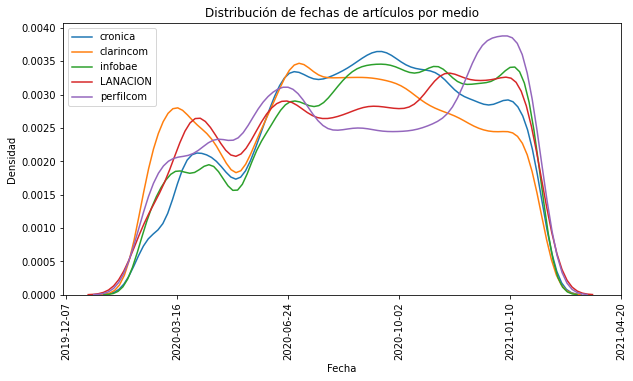
\includegraphics[width=\textwidth]{img/fechas_por_medios_todas.png}
        \caption{Distribución temporal de artículos recolectados, sin aplicar ningún filtro}
        \label{fig:fecha_articulos_por_medio_todas}
    \end{subfigure}

    \begin{subfigure}[t]{\textwidth}
        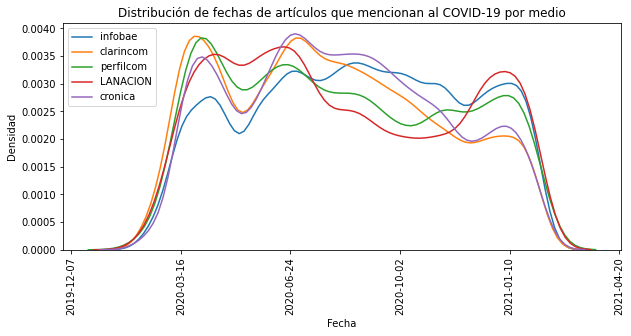
\includegraphics[width=\textwidth]{img/fechas_por_medios.png}
        \caption{Distribución temporal de artículos recolectados que mencionan COVID-19 o algún término relacionado}
        \label{fig:fecha_articulos_por_medio_covid}
    \end{subfigure}

    \caption{Gráficos de distribución de los datos recolectados. La figura \ref{fig:fecha_articulos_por_medio_todas}}
\end{figure}


\section{Recursos utilizados}

El etiquetado constó de XXX horas. A cada etiquetador le fue pagado YYYY por hora, y luego ZZZ por hora en segunda instancia. Esto equivale a WWW USD.

\section{Manual de criterios de anotación}
\label{app:manual_criterios_anotacion}
\chapter{Manual de criterios de anotación}
\label{app:manual_criterios_anotacion}
\section{Presencia de lenguaje discriminatorio}

Entendemos que hay discurso discriminatorio en el tweet si contiene declaraciones de carácter intenso y posiblemente irracional de rechazo, enemistad y aborrecimiento contra un individuo o contra un grupo, siendo estos objetivos de estas expresiones por poseer (o aparentar poseer) una característica protegida.

Este discurso puede manifestarse de manera explícita (insultos directos), celebraciones sobre asesinatos u otros crímenes, o bien otras expresiones más veladas. Lo que queremos captar es la intención del autor del tweet. El carácter discriminatorio de un mensaje está dado tanto por el contexto (en este caso, el tweet original del medio periodístico y posiblemente la nota) y el contenido del tweet en sí mismo. Por ejemplo, un comentario que diga “excelente” sin contexto es una cosa, y decir eso mismo en una nota que relata un femicidio, o un asesinato es otra muy distinta.

Las características protegidas que vamos a tener en cuenta son las siguientes:

\begin{enumerate}
\item Sexo (Mujeres, concretamente)
\item Género o identidad sexual (Colectivo LGBTI)
\item Ser inmigrantes, extranjeros, pueblos aborígenes u otras nacionalidades (Xenofobia, racismo)
\item Situación socioeconómica o por barrio de residencia
\item Poseer discapacidades, problemas salud mental o de adicción al alcohol u otros estupefacientes
\item Opinión o ideología política
\item Aspecto o edad (mayormente, gordofobia/gerontofobia)
\item Antecedentes penales o estar privado de la libertad

\end{enumerate}

Es decir, para considerar un mensaje como discriminatorio, debe cumplir que el discurso discriminatorio está orientado hacia un individuo o grupo de al menos una (aunque posiblemente más de una) característica protegida.


Consideramos que el mensaje del tweet (a la vez que el receptor del odio) es el que determina si puede o no ser considerado discriminatorio y hacia qué grupo está dirigido. Esto puede no necesariamente coincidir con el destinatario explícito del mensaje: por ejemplo, si alguien le dice a Susana Giménez “judía sionista hdp”, a pesar de no ser Susana Giménez judía, se puede considerar esto como discurso de odio contra las minorías religiosas y/o discurso xenófobo.


\section{Llamado a la acción}

Entendemos que un tweet (que contiene discurso discriminatorio) llama a la acción si contiene alguna incitación a tomar algún tipo de medida contra el sujeto o grupo ofendido. Esta medida puede ser de carácter violento (“hay que matarlos ya” “pongámosles una bomba”) o de carácter menos violento (“hay que dejar de comprarles a estos chinos ladrones”)

Estos tweets nos interesan particularmente porque son los más peligrosos y dañinos: los que llaman a tomar algún tipo de represalia contra la persona o el grupo en cuestión.

\section{Características protegidas}

Finalmente, para cada tweet deberemos marcar qué grupo o característica protegida es atacado. En este caso, necesariamente un grupo/característica debe ser seleccionado:

Usaremos una notación abreviada en la interfaz de etiquetado, en la que algunos de los grupos o características mencionadas fueron reagrupadas de la siguiente manera:

\begin{enumerate}
    \item MUJER: por su sexo
    \item LGBTI: por género o identidad sexual
    \item RACISMO: Por ser inmigrantes, extranjeros, pueblos aborígenes u otras nacionalidades (Xenofobia, racismo)
    \item POBREZA: Por situación socioeconómica o por barrio de residencia.
    \item DISCAPAC: Por tener discapacidades, problemas salud mental o de adicciones
    \item POLITICA: Por su opinión o ideología política
    \item ASPECTO: Por su aspecto o edad
    \item CRIMINAL: Por sus antecedentes o situación penal (presos)
\end{enumerate}

A su vez, agregamos la categoría “OTROS”. Esta categoría es excepcional, y debería utilizarse sólo si algún tipo de discriminación no está contemplado en estas categorías.

Respecto a la discriminación de carácter político tiene que ser algo más que una mera opinión  sino tener una componente irracional, de descalificación y de aborrecimiento considerable sobre un individuo o una facción política.

No se contempla dentro de las categorías protegidas a las profesiones. Es decir, no tenemos en cuenta el discurso contra científicos, médicos, o periodistas; de esto último hay bastante material agresivo en los comentarios.


\subsection{Lineamientos generales}

El discurso discriminatorio no es sólo discurso ofensivo contra una persona o grupo con alguna de las características protegidas. Tiene que apelar a su condición de mujer, inmigrante, LGBTI, etc. para que lo consideremos así.

Por ejemplo: si alguien agrede a una mujer, a un inmigrante, o a alguien de la comunidad LGBTI, no necesariamente está incurriendo en un discurso discriminatorio salvo que apele a algo que remita a su característica como tal.


Expresiones de aprobación ante noticias de crímenes o acciones contra persona o grupo de las características protegidas son consideradas discriminatorias.

\subsubsection{Ejemplos}

Violan a la reconocida actriz XXXX YYYY
Asesinan a un comerciante chino por creer que tenía Coronavirus
Motín y muerte en la prisión de Marcos Paz

Comentarios de contenido discriminatorio: (emoji de aplausos) - uno menos - bravo! -


Si no queda claro que haya un mensaje discriminatorio o parece de carácter difuso o demasiado tangencial, entonces etiquetar como no discriminatorio




\subsection{MUJER}

Insultar a una mujer sin hacer ninguna referencia particular a su condición de mujer no es suficiente para ser considerado discurso discriminatorio

Como regla: si el mismo insulto o agresión aplicase contra un hombre, entonces no debiéramos considerarlo como discriminación


Insultos contra las expresiones políticas del movimiento de las mujeres son consideradas en esta categoría: si se las insulta como feminazis, aborteras, pañuelito verde, etc



Apelaciones a su apariencia o aspecto propias de una mujer son consideradas en esta categoría. En este punto consideramos comentarios cosificadores


Insultar como “vieja” a una persona no califica como misoginia. Usar para ese caso la categoría ASPECTO que contempla la gerontofobia

EJEMPLOS:

Nati Jota furiosa por los comentarios que recibe en las redes.

Comentarios sexistas:

Pero si sos de plástico nena! (opina de manera denigratoria de su apariencia)
Flor de gato!
Miauuu!
A esta sólo se la conoce por su cuerpo y ahora se hace la santa. Andá a estudiar
Le damos hasta que San Lorenzo vuelva a Boedo
Y esta rubia tarada quién es?



Comentarios ofensivos pero no sexistas:
Callate forra (ofensivo pero no particularmente sexista)
Y esta quién es? A quién le importa?
Quién?
Nati cuánto?
Esta también recibe sobres?
Otra descerebrada más (súper agresivo, pero es un comentario que podría recibir un hombre, aunque en menor cantidad…)
Andá a cagar..boluda..conductora de 4ta..
HDP
Boba



\subsection{LGBTI}

Expresiones de disgusto o rechazo del estilo “qué asco” frente a integrantes de la colectividad deben ser marcados como discurso discriminatorio


Apelaciones a la anatomía o del estilo “biologicistas” deben ser marcados como discurso discriminatorio


Ejemplos:

Anibal Pachano sobre la cuarentena: “este virus nos está destruyendo a los actores”


Comentarios discriminatorios:

Qué asco este sujeto
Y a este trolo quién le pidió su opinión?
Me desagrada


Comentarios ofensivos pero no discriminatorios:

Ajá, y?
No me importa tu opinión, gracias
Se acuerdan cuando este atacaba a Cristina? Andá a llorarle al gato, Aníbal
Pelotudazo!


Famosa actriz trans dio una entrevista a La NACION: “Como mujer, estoy en la mejor etapa de mi vida”


Comentarios discriminatorios:

Muy lindo todo, pero sos hombre
“Mujer” dice jajajaj naciste y morirás macho
Qué asco este trolo
(emoji de asco)
Una mujer con sorpresa
Trava horrendo
Perdón pero qué nombre dice tu DNI?


Comentarios ofensivos pero no discriminatorios:

Quién?
Y a quién le interesa lo que diga esta mujer?
Que se vaya a cagar
Agradecele al gobierno de Néstor que tenés derechos





\subsection{RACISMO}

Asignar a todo un pueblo con una característica o actividad particular negativa entra en esta categoría
Cualquier llamada a expulsar, matar, tirar bombas, destruir, aniquilar, etc a un pueblo, inmigrantes o país entra en esta categoría. Más aún, deben ser marcadas como “llamadas a la acción”
Teorías conspirativas (hasta cierto punto) o acusaciones a un Gobierno/Estado no deberían entrar en esta categoría
¿Acusaciones respecto al virus?



Ejemplos:

Rescatan en China a cuarenta gatitos bebé que iban a ser utilizados en restaurantes


Comentarios discriminatorios:

Chinos asquerosos
Malparidos! Chinos de mierda
Sigan desparramando pestes hijos de puta!
Por qué no se comen entre ellos?
País horrible y enfermo
Estos chinos nos diseminan su peste por todo el mundo

Comentarios discriminatorios y que además llaman a la acción:

Son una plaga estos chinos, hay que matarlos a todos
Ojalá les caigan veinte bombas
Hay que barrer ese país de la faz de la tierra

Comentarios ofensivos pero no racistas:

Son comunistas, qué querés
Lo rescataron a Mauri?




Otros comentarios no racistas

El gobierno chino está intentando controlar todo, cuidado
Mienten con que controlaron el virus, cómo no van a mentir con esto también?
De terror!


Tomas de terrenos: se profundizan las tomas en todo Buenos Aires


Comentarios discriminatorios:

Rajen a todos los peruanos de las tomas! (llama a la acción, además)
Increíble, cualquier paraguayo o bolita de mierda te saca la casa

\subsection{POBREZA}

Expresiones denigrantes sobre la condición socioeconómica son consideradas discriminatorias: referirse a las personas sin empleo como “vagos”, a otros como “(chori)planeros”
Respecto a la gente que posee planes de asistencia social, si es una opinión general sin ser ofensiva no se considera discriminatoria (del estilo “hay que reducir el gasto social y los planes”, “perdieron la cultura del trabajo”)

Presupuesto: aumentó el gasto en planes asistenciales durante la pandemia

Ejemplos discriminatorios:

Basta de mantener vagos!
Cansada de los planeros
Che laburar estos atorrantes ni en pedo no?
PARASITOS

Ejemplos no discriminatorios

La gente que trabaja y aporta impuestos es cada vez menos. Estamos al horno



\subsection{POLITICA}

Apreciaciones derogatorias sobre la posición política son consideradas discriminatorias : zurdo/a, bolchevique, peroncho, gorila, kuka, etc
Acusaciones de corrupción o de “recibir sobres” no son consideradas discriminatorias
Tampoco aquellas expresiones que traten de inútiles a funcionarios
Tratar de viejo/a, gordo/a, u otras cuestiones físicas deben ser marcados en las categorías respectivas, no acá

Aumentó el gasto en planes asistenciales durante la pandemia

Ejemplos discriminatorios:

BASTA ZURDOS DE ROBARNOS
Bolcheviques de mierda

Ejemplos no discriminatorios

La gente que trabaja y aporta impuestos es cada vez menos. Estamos al horno
Qué gobierno de inútiles
Son unos delincuentes
Hijos de mil puta!
Siguen volando los sobres para el Congreso
Siga siga la impresión




\subsection{ASPECTO}

Apreciaciones denigrantes sobre la apariencia de una persona y/o su edad
Principalmente, tenemos en mente la gordofobia y gerontofobia, pero puede referir a otras características físicas (por ejemplo, la altura)
En casos en las cuales haya solapamiento con mujer, marcar ambas


Luis Brandoni: “No convoqué el banderazo”

Ejemplos discriminatorios:

Viejo de mierda!
Qué decrépito impresentable que es este señor
Estás gagá, pelotudo

Jorge Lanata vuelve a la televisión

Ejemplos discriminatorios:

Gordo chanta otra vez volvés a vender pescado podrido?
porque no te vas vos tambien con todos bola de sebo!!!1
Estás gagá, pelotudo









\subsection{CRIMINAL}

Cualquier comentario que celebre acciones contra criminales o personas privadas de su libertad (golpizas, asesinatos, muerte en motines, etc) entra en esta categoría
En este ítem muchas veces veremos que son llamados a la acción: el de “matarlos”, llamar a reducir sus derechos, etc
Muere un delincuente tras un enfrentamiento con la policía

Ejemplos discriminatorios:

Uno menos!
Excelente!
(emoji de aplausos)
Que pena, pobrecito

Ejemplos que además llaman a la acción

MUY BIEN! Felicitaciones al policía, hay que liquidarlos sin piedad


1...100 101..200 …. 501...600

Primera fase: Et 1 => 1..100, Et 2 => 101 .. 200 … Et 6 => 501..600
Segunda fase Et2 => 1..100 Et1 => 101..200…. Et 6 => 401..500 Et 5 => 501..600

Shufflear temporalmente

Ejemplos no discriminatorios


Cómo puede ser que nuestra Ministra no haga nada?
La policía actuó correctamente.

Motín por el Coronavirus en Olmos: 3 muertos

Ejemplos discriminatorios y que llaman a la acción

Hay que rociar con nafta todas las cárceles
Soltemos 3 o 4 infectados con COVID en cada cárcel y problema solucionado
Paredón y listo



\subsection{DISCAPACIDAD}

Referencias peyorativas de adicciones a drogas, alcohol u otros estupefacientes
También referencias peyorativas a la salud mental de la persona en cuestión
Decir “está loco” no entra acá :-)
Malena Pichot sale a cruzar a Baby Etchecopar
Ejemplos discriminatorios:

Callate faloperita!
Jorge Lanata vuelve a la televisión

Ejemplos discriminatorios:

Che no probaste dejar la merca gordo?

Noticia sobre Patricia Bullrich...

Ejemplos discriminatorios:

Largá la (emoji de botella) Pato
Borracha hdp



\subsection{OTROS}

Esta categoría está reservada para cualquier otro tipo de discriminación que no esté contemplada en las categorías mencionadas
Insultos a profesiones (científicos, periodistas, por ejemplo) no entran en este apartado
ESTA CATEGORIA ES SUMAMENTE EXCEPCIONAL. NO USAR INDISCRIMINADAMENTE


\chapter{Apéndice Capítulo 6}
\label{app:06}

En este apéndice incluímos tablas y resultados completos


\section{Análisis comparativo entre clasificadores granulares y binarios}


\begin{table}[ht!]
    \centering
    \footnotesize
    \tbf{LGBTI}
    \begin{tabular}{p{0.03\textwidth} p{0.05\textwidth} p{0.45\textwidth} p{0.40\textwidth}}
        \hline
        1 & FN & Mara Gómez: la historia de la primera futbolista trans en el torneo argentino & Ponga huevos, Mara ponga huevos... \\
        2 & FN & Graciana Peñafort: "La marcha me dio mucha pena y tuvo un nivel de convocatoria menor al esperado" & Pena das vos, termotanque de lipídos y déficit fiscal \\
        3 & FP & "No soy feminista, soy mujer ", la frase de Viviana Canosa que generó polémica & La condición de mujer no la exime de ser una pelotuda y terrible hija de puta. Asi como tampoco la exime de vivir en un mundo con menos oportunidades, menores remuneraciones y más riesgos x el solo hecho de ser mujer, aunque no quiera luchar x eso. \\
        4 & FP & T ras una ráfaga de más de 20 disparos asesinaron a una mujer trans en Rosario & Con que le dispararon? Alta minigun tiene que ser para que 20 tiros sean solo una ráfaga y no una fullauteada \\
    \end{tabular}
    \tbf{RACISMO}
    \begin{tabular}{p{0.03\textwidth} p{0.05\textwidth} p{0.45\textwidth} p{0.40\textwidth}}
        1 & FN & Es hija de chinos, llevó merienda al colegio para compartir y se la rechazaron por temor a contagiarse de coronavirus &  Con lo hijos de puta, maleducados e intransigentes que son los chinos, si fuese al revés ya nos hubiesen embarcado a la estratosfera. Nadie ha visto como echan a los chicos pobres de los super por el miedo a que los afanen? Hablando de prejuicios \\
        1 & FN & Multitudes en las calles y discotecas abarrotadas: la fiesta de Wuhan tras el año de la pandemia que se inició en uno de sus "mercados húmedos" &  Los odio \\
        1 & FN & Su novia es mexicana y Migraciones le exige casi 50 mil pesos para dejarla ingresar a la Argentina &  Mira si le cobran eso a cada venezolano colombiano peruano chino boliviano que vienen al país a chupar sangre ,pagamos la deuda externa y nos volvemos potencia mundial \\
        1 & FP & URGENTE: Un hombre se incrustó con su auto en la puerta de la Embajada de China y aseguró que tenía explosivos & No es hombre . Es un boludo \\
        1 & FP & Su novia es mexicana y Migraciones le exige casi 50 mil pesos para dejarla ingresar a la Argentina &  Que me traiga una botellas de tequila del bueno \\
        1 & FP & El principal gremio docente nacional rechazó el regreso a las clases presenciales &Banda de VAGOS \\
        1 & FP & China: identificaron otro virus "con potencial para convertirse en pandemia" nuevo virus china transportado por cerdos podría infectar ahumanos las actuales vacunas podrían adaptarse más en la nota & PERO LA PUTA MADRE VIEJO \\
    \end{tabular}
    \caption{Ejemplos donde el clasificador granular acierta y el binario falla. FN marca que el clasificador binario no detecta el comentario como discriminatorio mientras que el contextualizado sí lo hace; FP es al revés, que el clasificador binario marca erróneamente el comentario como discriminatorio. Agrupadas de acuerdo a ciertas características; en el caso de los falsos positivos esta categoría es especulativa}
    \label{tab:fine_vs_plain_comparison}
\end{table}
% Capítulo 7 - Tablas de resultados de ajuste de dominio
\chapter{Adaptación de dominio}
\label{app:07}


En la tabla \ref{tab:full_domain_adaptation_evaluation_results} tenemos los resultados para todos los modelos considerados en el benchmark de adaptación de dominio, referidos en la sección \ref{sec:domain_adaptation_results}. Notamos, para compacidad, con subíndice \emph{U, C, D} a las versiones  \emph{uncased}, \emph{cased} y \emph{deacc}. Así mismo, notamos con $10K$ (por ejemplo) a aquel modelo con adaptación de dominio por 10,000 pasos según descripto en la sección \ref{sec:domain_adaptation_vs_robertuito}.

Podemos observar que, observando el score general, el mejor modelo adaptado a dominio para las versiones \emph{uncased} es beto$_{U10K}$, y para las versiones \emph{cased} es \beto{}$_{C5K}$; si bien en este último caso tiene una performance muy similar al de 20K pasos (de hecho, omitiendo la tarea de discurso de odio contextualizado gana por mínimo margen el de 20K).

\begin{sidewaystable}
    \centering
    \large
    \begin{tabular}{llllllr}
        \toprule
        Modelo             & CHATE                   &  HATE              &  SENTIMENT        &  EMOTION          &  IRONY            &     score \\
        \midrule
        beto$_{U5K}$   & $0.557 \pm 0.007$ & $0.756 \pm 0.012$ & $0.654 \pm 0.005$ & $0.509 \pm 0.014$ & $0.684 \pm 0.007$ &  0.632 \\
        beto$_U$        & $0.591 \pm 0.006$ & $0.757 \pm 0.012$ & $0.649 \pm 0.005$ & $0.521 \pm 0.006$ & $0.702 \pm 0.008$ &  0.644 \\
        bertin          & $0.557 \pm 0.008$ & $0.767 \pm 0.005$ & $0.665 \pm 0.003$ & $0.518 \pm 0.012$ & $0.716 \pm 0.008$ &  0.645 \\
        beto-cased      & $0.582 \pm 0.007$ & $0.768 \pm 0.012$ & $0.665 \pm 0.004$ & $0.521 \pm 0.012$ & $0.706 \pm 0.007$ &  0.648 \\
        roberta-bne     & $0.577 \pm 0.004$ & $0.766 \pm 0.015$ & $0.669 \pm 0.006$ & $0.533 \pm 0.011$ & $0.723 \pm 0.017$ &  0.653 \\
        beto$_{C2.5K}$  & $0.580 \pm 0.005$ & $0.771 \pm 0.007$ & $0.677 \pm 0.006$ & $0.525 \pm 0.010$ & $0.717 \pm 0.008$ &  0.654 \\
        beto$_{C10K}$   & $0.574 \pm 0.008$ & $0.782 \pm 0.009$ & $0.680 \pm 0.006$ & $0.524 \pm 0.006$ & $0.720 \pm 0.007$ &  0.656 \\
        beto$_{C20K}$   & $0.572 \pm 0.006$ & $0.777 \pm 0.009$ & $0.686 \pm 0.005$ & $0.517 \pm 0.009$ & $0.730 \pm 0.004$ &  0.656 \\
        beto$_{C5K}$    & $0.576 \pm 0.002$ & $0.781 \pm 0.010$ & $0.677 \pm 0.004$ & $0.525 \pm 0.016$ & $0.724 \pm 0.009$ &  0.657 \\
        beto$_{U20K}$   & $0.588 \pm 0.007$ & $0.768 \pm 0.012$ & $0.684 \pm 0.005$ & $0.533 \pm 0.016$ & $0.712 \pm 0.009$ &  0.657 \\
        beto$_{U2.5K}$  & $0.588 \pm 0.004$ & $0.784 \pm 0.011$ & $0.676 \pm 0.005$ & $0.533 \pm 0.008$ & $0.715 \pm 0.007$ &  0.659 \\
        beto$_{U10K}$   & $0.588 \pm 0.003$ & $0.775 \pm 0.015$ & $0.680 \pm 0.004$ & $0.553 \pm 0.009$ & $0.717 \pm 0.005$ &  0.663 \\
        robertuito$_C$  & $0.590 \pm 0.005$ & $0.790 \pm 0.012$ & $0.701 \pm 0.012$ & $0.519 \pm 0.032$ & $0.719 \pm 0.023$ &  0.664 \\
        robertuito$_{D}$& $0.593 \pm 0.006$ & $0.798 \pm 0.008$ & $0.702 \pm 0.004$ & $0.543 \pm 0.015$ & $0.740 \pm 0.006$ &  0.675 \\
        robertuito$_U$  & $0.593 \pm 0.004$ & $0.801 \pm 0.010$ & $0.707 \pm 0.004$ & $0.551 \pm 0.011$ & $0.736 \pm 0.008$ &  0.678 \\
        \bottomrule
    \end{tabular}
    \caption{Resultados de la evaluación de modelos pre-entrenados y modelos ajustados en dominio para el benchmark de tareas sociales: CHATE es contextualized hate speech, HATE es hate speech detection sobre el dataset de hatEval, SENTIMENT, EMOTION e IRONY son análisis de sentimiento, emociones e ironía sobre los corpus de TASS. Todos los scores son Macro F1s. beto-cased-ft y beto-uncased-ft son modelos adaptados al dominio sociall. Score es la media de cada fila. Gap es.. delta es...}

    \label{tab:full_domain_adaptation_evaluation_results}

\end{sidewaystable}





%%%% BIBLIOGRAFIA
\backmatter
\bibliography{biblio.bib}

\end{document}
